\chapter{Background}
\label{ch:bg}

\epigraph{
Anyone who considers arithmetical methods of producing random digits is, of course, in a state of sin.
}
% For, as has been pointed out several times, there is no such thing as a random number --- there are only methods to produce random numbers, and a strict arithmetic procedure of course is not such a method.
{\textsc{John von Neumann}}


\section{Sequential Monte Carlo}
The idea of Monte Carlo is to use (pseudo-)random numbers to approximate expectations under an intractable probability distribution of interest.
Sequential Monte Carlo (SMC) is a class of Monte Carlo algorithms which are implemented sequentially, allowing efficient sampling from sequences of distributions.
SMC was developed for inference in intractable state space models (details in Section~\ref{sec:SSMs}) and introduced to the statistics community by \textcite{gordon1993}.
The basic idea behind SMC is that of sequential importance sampling, whereby the importance samples from one target distribution are used to generate proposals for the next. A full derivation of the SMC recursions is beyond the scope of this work, but the reader is referred to e.g.\ \textcite{doucet2009, chopin2020} for more background. Here it suffices to provide a motivation in the context of state space models (Section~\ref{sec:SSMs}) and the formalism of Feynman-Kac models (Section~\ref{sec:FKmodels}).





\subsection{State space models}
\label{sec:SSMs}
State space models (sometimes called hidden Markov models) are a flexible class of statistical models which are suitable in all sorts of applications where observations appear sequentially.
\begin{figure}[ht]
\centering
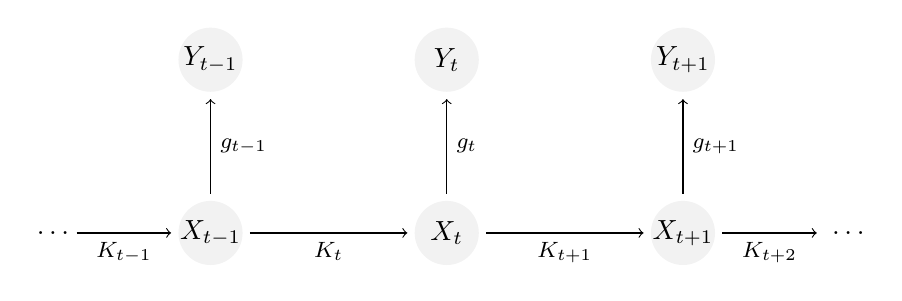
\begin{tikzpicture}
\filldraw[gray!10] (-3,0) circle (0.4);
\filldraw[gray!10] (-3,2.2) circle (0.4);
\filldraw[gray!10] (0,0) circle (0.4);
\filldraw[gray!10] (0,2.2) circle (0.4);
\filldraw[gray!10] (3,0) circle (0.4);
\filldraw[gray!10] (3,2.2) circle (0.4);
\node at (3,2.2) {$Y_{t+1}$};
\node at (3,0) {$X_{t+1}$};
\node at (0,2.2) {$Y_{t}$};
\node at (0,0) {$X_{t}$};
\node at (-3,2.2) {$Y_{t-1}$};
\node at (-3,0) {$X_{t-1}$};
\node at (-5,0) {$\dots$};
\node at (5.1,0) {$\dots$};
\draw[->] (-4.7,0)-- node[anchor=north] {\footnotesize{$K_{t-1}$}} (-3.5,0);
\draw[->] (-2.5,0)-- node[anchor=north] {\footnotesize{$K_t$}} (-0.5,0);
\draw[->] (0.5,0)-- node[anchor=north] {\footnotesize{$K_{t+1}$}} (2.5,0);
\draw[->] (3.5,0)-- node[anchor=north] {\footnotesize{$K_{t+2}$}} (4.7,0); 
\draw[->] (-3,0.5)-- node[anchor=west] {\footnotesize{$g_{t-1}$}} (-3,1.7);
\draw[->] (0,0.5)-- node[anchor=west] {\footnotesize{$g_t$}} (0,1.7);
\draw[->] (3,0.5)-- node[anchor=west] {\footnotesize{$g_{t+1}$}} (3,1.7);
\end{tikzpicture}
\caption[State space model]{Conditional independence graph for a general state space model. $(X_t)$ is a Markov process with transition kernels $(K_t)$ representing the underlying state of the system. $Y_t$ is a noisy observation of $X_t$ for each $t$.}
\label{fig:SSM}
\end{figure}
The general model has two components: a Markov process $(X_t)_{t\in\mathbb{N}_0}$ representing the (unobservable) underlying state of the system, and a sequence $(Y_t)_{t\in\mathbb{N}_0}$ of observations containing information about the underlying state. The model is characterised by its conditional independence structure (Figure~\ref{fig:SSM}) along with an initial distribution $\mu$, the Markov ``transition'' kernels $(K_t)_{t\in\mathbb{N}}$ and the ``emission'' distributions $(g_t)_{t\in\mathbb{N}_0}$. 
Written as a hierarchical model,
\begin{align}
X_0 &\sim \mu(\cdot) & \notag\\
X_{t+1} \mid X_t &\sim K_{t+1}(\cdot | X_t) & \text{for } t=0, 1, \dots
        \label{eq:SSM_spec}\\
Y_t \mid X_t &\sim g_t(\cdot | X_t) & \text{for } t=0, 1, \dots \notag
\end{align}
The index $t$ will frequently be referred to as ``time'', since in many applications the sequence is indeed a time series, but it need not be.

Here $X$ and/or $Y$ may be multivariate and observation times need not be equally spaced. Straightforward generalisations of the stated model can allow for situations in which observations are not available as often as the state is updated (up to and including the extreme where the state is a continuous-time Markov process but the observations are available only at discrete times) or on the other hand where observations are made more frequently than the state is updated.

Applications include target tracking, where $X$ is the true position of some object and $Y$ encodes some measurements from sensors e.g.\ radar; stochastic volatility models, where $X$ is the volatility and $Y$ is the observed value e.g.\ the price of a stock; change-point detection; and many other situations in which there is an observed time series from which one would like to do inference or prediction.

The principal inferences of interest in state space models are:
\begin{description}
\item [filtering] $p(x_t\mid y_{0:t})$: inferring the current state $x_t$ from the observations up to now $y_{0:t}$
\item [prediction] $p(x_{t+h}\mid y_{0:t})$: inferring a future state $x_{t+h}$ from the observations up to now $y_{0:t}$
\item [(complete) smoothing] $p(x_{0:t}\mid y_{0:t})$: inferring the sequence of states up to now $x_{0:t}$ from the observations up to now $y_{0:t}$
\item [fixed-lag smoothing] $p(x_{t-h:t}\mid y_{0:t})$: inferring the last $h$ states $x_{t-h:t}$ from the observations up to now $y_{0:t}$
\end{description}
If the dynamics of the state space model are parametrised by some $\theta$, i.e.\ $g_t$ and/or $K_t$ depend on $\theta$, we may also be interested in parameter inference or computing the likelihood $p(y_{0:t})$ of the observed data for particular values of $\theta$. Such a model is considered in Section~\ref{sec:particleGibbs}.

In certain cases, these inference problems may be solved analytically (Section~\ref{sec:SSM_exact_inference}), but this is not typically the case. For intractable models we must resort to numerical methods such as Monte Carlo. However, state space inference is problematic even with Monte Carlo. 
The main difficulties are that the dimension of the target distributions may increase along the sequence, and that there is strong dependence between consecutive distributions. Markov chain Monte Carlo (MCMC), for instance, is known to struggle with highly correlated targets%\seb{[citation]} 
and its performance drops drastically as dimension increases, despite convergence rates that are independent of dimension.%\seb{[citation]}

As we will see in Section~\ref{sec:SMC_FK}, sequential Monte Carlo somewhat overcomes these problems, turning the problematic properties of the target distribution to its benefit. Correlation between consecutive targets is exploited for sequential updating, which is able to handle the incrementing dimensionality. The resulting linear-in-$t$ computational complexity also allows inference to be performed on-line, that is, updating the posterior distribution(s) as observations arrive.




\subsection{Inference in state space models}
\label{sec:SSM_exact_inference}
If the state space model has linear dynamics with Gaussian noise, the posterior distributions of interest are also Gaussian. The posterior mean and covariance satisfy certain recursions, implemented by the Kalman filter \parencite{kalman1960} and Rauch-Tung-Striebel smoother \parencite{rauch1965}. 
Recursions are also available for some other conjugate models: see for example \textcite{vidoni1999,king2021}.
Another analytic case occurs if the state space $\mathcal{X}$ is finite, in which case any integrals become finite sums, and the forward-backward algorithm \parencite{baum1970} yields the exact posteriors. However, if the state space becomes large, albeit finite, exact computation becomes infeasible.

If the model is Gaussian but non-linear, the posterior filtering distributions can be estimated using the \emph{extended Kalman filter} (see for example \textcite{jazwinski2007}), which applies a first-order approximation in order to make use of the Kalman filter. This method performs well on models that are ``almost linear''. The resulting predictor is only \emph{optimal} when the model is actually linear, in which case the extended Kalman filter coincides with the Kalman filter.

For models that are high-dimensional or highly non-linear or for which gradients are not readily available, the exact Kalman filter updates can be replaced by sample approximations.
The \emph{ensemble Kalman filter} \parencite{evensen1994} uses a Monte Carlo sample from the current time, propagates these points through the transition dynamics, and uses the sample covariance as an estimator of the updated covariance matrix. The means, which are cheaper to evaluate and more stable than the covariances, are still updated using the Kalman filter recursion, based on the estimated covariance.
The \emph{unscented Kalman filter} \parencite{wan2000} uses a deterministic sample chosen via the \emph{unscented transformation}, which is then propagated through the non-linear transition kernel to obtain a characterisation of the distribution at the next time step. The sample consists of $2d+1$ points, where $d$ is the dimension of the state space, and defines a Gaussian approximation to the updated distribution. If the model is really linear-Gaussian then the sample points are sufficient to recover the correct distribution.

In complex or high-dimensional models, exact inference is often infeasible, and we turn instead to Monte Carlo methods.
Markov chain Monte Carlo performs woefully on state space models due to the high dimension of the parameter space and high correlation between dimensions. 
But we can exploit the sequential nature of the underlying dynamics to decompose the problem into a sequence of inferences of fixed dimension.
This is the motivation behind sequential Monte Carlo (SMC).


\subsection{Feynman-Kac models}
\label{sec:FKmodels}
%\seb{Give example of non-SSM that is FK? Obvious options are SMC samplers e.g.\ for rare event simulation or sequential ABC or tempering.}\\
State space models are very natural and intuitive applications, but they do not do justice to the scope of SMC algorithms, which is much wider.
On the other hand, 
%the \emph{Feynman-Kac} formalism captures the full scope, since 
every SMC algorithm is a Monte Carlo approximation of some \emph{Feynman-Kac} model.
Before formally introducing SMC let us therefore define a generic Feynman-Kac model.
For a more in-depth study, the reader is directed to the exhaustive books by \textcite{delmoral2004, delmoral2013} or the more accessible \textcite[Chapter 5]{chopin2020}.

Define a state space $\mathcal{X}$, which in this presentation we assume to be common for all times: this is often not the case in practice, but the generalisation to a sequence of state spaces is straightforward.
The basic components of the Feynman-Kac model are a Markov law, defined by an initial distribution $\mathbb{M}_0$ on $\mathcal{X}$ and transition kernels $M_t: \mathcal{X} \mapsto \mathcal{X}$ for $t\in\mathbb{N}$; and a sequence of \emph{potential} functions $G_0 : \mathcal{X} \mapsto [0,\infty)$  and $G_t : \mathcal{X}^2 \mapsto [0,\infty)$ for $t\in\mathbb{N}$.
From these we can construct, for any time horizon $T$, a sequence of Feynman-Kac measures $(\mathbb{Q}_t)_{t=0:T}$ defined by the changes of measure
\begin{equation}
\mathbb{Q}_t (dx_{0:T}) = \frac{1}{L_t} G_0(x_0) \mathbb{M}_0(dx_0)
        \left\{ \prod_{s=1}^t G_s(x_{s-1}, x_s) \right\} 
        \left\{ \prod_{s=1}^T M_s(x_{s-1}, dx_s) \right\} , \label{eq:FKmeasure}
\end{equation}
where $L_t$ is the normalising constant required to make $\mathbb{Q}_t$ a probability measure. Other quantities such as $\mathbb{Q}_t (dx_{0:t})$ can be obtained as marginals of \eqref{eq:FKmeasure}, allowing us to treat all of the inference problems described in Section~\ref{sec:SSMs} by approximating $\mathbb{Q}_t$ and then possibly marginalising.

The generic state space model defined in \eqref{eq:SSM_spec} may be described by a Feynman-Kac model where:
\begin{align}
\mathbb{M}_0 &:= \mu \notag\\
M_t (x_{t-1}, dx_t) &:= K_t (dx_t \mid x_{t-1}) & \text{for } t=1,2,\dots \notag\\
G_0 (x_0) &:= g_0 ( y_0 \mid x_0 ) \notag\\
G_t (x_{t-1}, x_t) &:= g_t( y_t \mid x_t ) & \text{for } t=1,2,\dots . \label{eq:bootstrapFK}
\end{align}
This is not the only Feynman-Kac model for \eqref{eq:SSM_spec}; this corresponds to the \emph{bootstrap} SMC algorithm, which is the simplest implementation.
Abusing notation, $g_t$ now denotes the density of the corresponding emission distribution; state space models in which these densities do not exist can still be expressed as Feynman-Kac models, the but not this bootstrap model.
In practice the bootstrap SMC algorithm may be significantly outperformed by more involved algorithms such as
\emph{auxiliary particle filters} \parencite{pitt1999, carpenter1999} and those using \emph{locally optimal proposals} \parencite[e.g.][]{doucet2000} or \emph{lookahead methods} \parencite{lin2013}.
Feynman-Kac formalisms for some of these variants are presented for example in \textcite[Section 5.1.2]{chopin2020}.

It remains to demonstrate that the measures $\mathbb{Q}_t$ arising from \eqref{eq:bootstrapFK} are sufficient for all the usual inference problems in the corresponding state space model \eqref{eq:SSM_spec}.
By construction, the complete smoothing distribution is precisely
\begin{align*}
\mathbb{Q}_t (dx_{0:t})
&= \frac{1}{L_t} G_0(x_0) \mathbb{M}_0(dx_0)
        \prod_{s=1}^t G_s(x_{s-1}, x_s) M_s(x_{s-1}, dx_s) \\
&= g_0(y_0 \mid x_0) \mu(dx_0) 
        \prod_{s=1}^t g_s(y_s \mid x_s) K_s(dx_s \mid x_{s-1}) \\
&= p(dx_{0:t} \mid y_{0:t}) . 
\end{align*}
The filtering, prediction and fixed-lag smoothing distributions are all also marginals of some $\mathbb{Q}_t(dx_{0:T})$:
\begin{align}
p(dx_t \mid y_{0:t}) &= \mathbb{Q}_t (dx_t) \notag\\
p(dx_{t+h} \mid y_{0:t}) &= \mathbb{Q}_t (dx_{t+h}) \label{eq:FK_marginals}\\
p(dx_{t-h:t} \mid y_{0:t}) &= \mathbb{Q}_t (dx_{t-h:t}) , \notag
\end{align}
while the likelihood $p(y_{0:t}) = L_t$.
This means that Monte Carlo approximation of $\mathbb{Q}_t(dx_{0:T})$ is sufficient for inference on any of these distributions, since marginalisation of Monte Carlo samples is trivial. The likelihood, on the other hand, is not obtained by marginalisation; nevertheless, we will see that likelihood estimates can also be obtained ``for free''. 
The next section describes how we may obtain Monte Carlo samples from $\mathbb{Q}_t(dx_{0:T})$.




\subsection{Sequential Monte Carlo for Feynman-Kac models}
\label{sec:SMC_FK}
In order to implement the SMC algorithm corresponding to a given Feynman-Kac model, we need to be able to sample from $\mathbb{M}_0$ and from $M_t(x, \cdot)$ for all $x,t$; and evaluate $G_t(x, y)$ pointwise for each $x,y, t$.
Under these conditions we may implement Algorithm~\ref{alg:SMC}, which describes a generic SMC algorithm. 
The only free choices are the parameter $N$ which dictates the number of ``particles'' used, and the \textsc{resample} procedure.
However, remember that given a particular state space model there is also a choice of possible Feynman-Kac descriptions, and this choice can strongly affect performance.

\begin{algorithm}[ht]
\vspace*{10pt}
\DontPrintSemicolon
\KwIn{$T, N, \mathbb{M}_0, (M_t)_{t=1}^T, (G_t)_{t=0}^T$}
\lFor{$i \in \{1,\dots,N\}$}{ 
	Sample $X_0^{(i)} \sim \mathbb{M}_0(\cdot)$
}
\lFor{$i \in \{1,\dots, N\}$}{
		$w_{0}^{(i)} \gets  \left\{{\sum_{j=1}^N G_0(X_0^{(j)})}\right\}^{-1}{G_0(X_0^{(i)})} $ 
	}
\For{$t \in \{1,\dots, T\}$}{
	Sample $a_{t-1}^{(1:N)} \sim $ \textsc{resample}$(\{1,\dots ,N\}, w_{t-1}^{(1:N)}$)\;
	\lFor{$i \in \{1,\dots,N\}$}{
		Sample $X_{t}^{(i)} \sim M_{t}(X_{t-1}^{(a_{t-1}^{(i)})}, \cdot)$
	}
	\lFor{$i \in \{1,\dots, N\}$}{	
		$w_{t}^{(i)} \gets \Big\{ {\sum_{j=1}^N G_{t}(X_{t-1}^{(a_{t-1}^{(j)})}, X_{t}^{(j)}) }\Big\}^{-1} G_{t}(X_{t-1}^{(a_{t-1}^{(i)})},X_{t}^{(i)}) $
	}
}
\vspace*{10pt}
\caption[Sequential Monte Carlo]{Sequential Monte Carlo for a generic Feynman-Kac model}
\label{alg:SMC}
\end{algorithm}

The choice of \textsc{resample} procedure can also have a profound effect on performance and is discussed in detail in Section~\ref{sec:resampling}. 
Resampling is not necessary for the algorithm to be valid, but it is important to ensure good performance. Its purpose is to periodically ``reset'' the weights $w_t^{(1:N)}$, preventing \emph{weight degeneracy}. This is the phenomenon that multiplying importance weights over time causes the variance of the unnormalised weights to increase exponentially, until after some iterations practically all of the weight is concentrated on one particle, with the rest having weights very close to zero. This means that the Monte Carlo sample (of size $N$) essentially consists of just one sample, so that the Monte Carlo approximations have very high variance.

The idea of resampling is to make multiple copies of particles with high weights and eliminate particles with low weights, then reset the weights to $w_t^{(1:N)} = (1,\dots,1)/N$. Done correctly, this procedure does not introduce any bias and, although it increases variance in the short term by adding extra randomness, it improves stability in the long term.
It also prevents computational budget being ``wasted'' on simulating low-weight particles which do not contribute much to the approximation.

For each $i=1,\dots,N$, the \textsc{resample} procedure selects a \emph{parent}, indexed by $a_{t-1}^{(i)} \in \{1,\dots,N\}$, which copies its state to the $i$th particle in the next iteration. These copies are then mutated independently and so the algorithm goes on.
We define the \emph{offspring counts} for each $i,t$ as
\begin{equation*}
\nu_{t-1}^{(i)} := |\{ j: a_{t-1}^{(j)} = i \}| ,
\end{equation*}
the number of copies in generation $t$ of particle $i$ from generation $t-1$ appearing by resampling. Notice that $\nu_{t-1}^{(1:N)}$ is expressed as a non-injective function of $a_{t-1}^{(1:N)}$, and as such carries less information.
To ensure Algorithm~\ref{alg:SMC} is valid, we assume that the resampling procedure
is \emph{unbiased}, that is, the expectation of $\nu_{t-1}^{(i)}$ is proportional to $w_{t-1}^{(i)}$ for each $i$. This requirement is formalised in Definition~\ref{defn:resampling}.
% satisfies the following properties: that the population size $N$ is conserved; and that, given $w_{t-1}^{(1:N)}$, the expectation of $\nu_{t-1}^{(i)}$ is proportional to $w_{t-1}^{(i)}$ for each $i$.
%The latter property is known as \emph{unbiasedness}.
%These requirements are made rigorous in Definition~\ref{defn:resampling}.

\begin{figure}[ht]
\centering
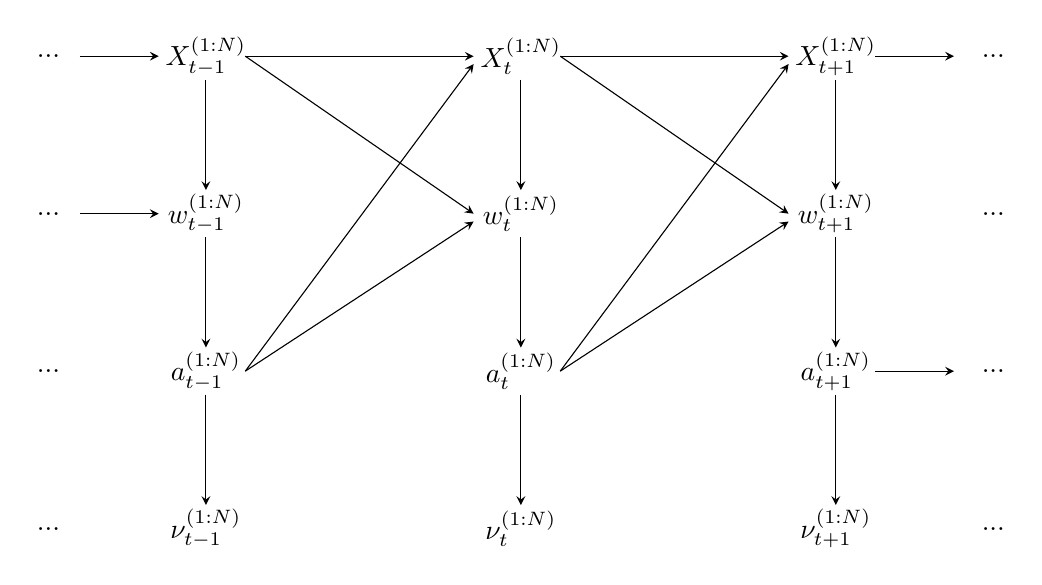
\begin{tikzpicture}[>=stealth]
% left dots
\node at (-2,0) {...};
\node at (-2,-2) {...};
\node at (-2,-4) {...};
\node at (-2,-6) {...};
% labels (t+1)
\node at (0,0) {$X_{t-1}^{(1:N)}$};
\node at (0,-2) {$w_{t-1}^{(1:N)}$};
\node at (0,-4) {$a_{t-1}^{(1:N)}$};
\node at (0,-6) {$\nu_{t-1}^{(1:N)}$};
% labels t
\node at (4,0) {$X_{t}^{(1:N)}$};
\node at (4,-2) {$w_{t}^{(1:N)}$};
\node at (4,-4) {$a_{t}^{(1:N)}$};
\node at (4,-6) {$\nu_{t}^{(1:N)}$};
% labels (t-1)
\node at (8,0) {$X_{t+1}^{(1:N)}$};
\node at (8,-2) {$w_{t+1}^{(1:N)}$};
\node at (8,-4) {$a_{t+1}^{(1:N)}$};
\node at (8,-6) {$\nu_{t+1}^{(1:N)}$};
% right dots
\node at (10,0) {...};
\node at (10,-2) {...};
\node at (10,-4) {...};
\node at (10,-6) {...};
% arrows (t+1) -> t
\draw[->] (0.5,0)--(3.4,0);
\draw[->] (0.5,0)--(3.4,-2);
\draw[->] (0.5,-4)--(3.4,-2.1);
\draw[->] (0.5,-4)--(3.4,-0.1);
% arrows t -> (t-1)
\draw[->] (4.5,0)--(7.4,0);
\draw[->] (4.5,0)--(7.4,-2);
\draw[->] (4.5,-4)--(7.4,-2.1);
\draw[->] (4.5,-4)--(7.4,-0.1);
% vertical arrows (t+1)
\draw[->] (0,-0.3)--(0,-1.7);
\draw[->] (0,-2.3)--(0,-3.7);
\draw[->] (0,-4.3)--(0,-5.7);
% vertical arrows t
\draw[->] (4,-0.3)--(4,-1.7);
\draw[->] (4,-2.3)--(4,-3.7);
\draw[->] (4,-4.3)--(4,-5.7);
% vertical arrows (t-1)
\draw[->] (8,-0.3)--(8,-1.7);
\draw[->] (8,-2.3)--(8,-3.7);
\draw[->] (8,-4.3)--(8,-5.7);
% arrows ... -> t+1
\draw[->] (-1.6,0)--(-0.6,0);
\draw[->] (-1.6,-2)--(-0.6,-2);
% arrows t-1 -> ...
\draw[->] (8.5,0)--(9.5,0);
\draw[->] (8.5,-4)--(9.5,-4);
\end{tikzpicture}
\caption[Conditional dependence structure of SMC algorithm]{Part of the conditional dependence graph implied by Algorithm~\ref{alg:SMC}. The direction of time is from left to right.}
\label{fig:cond_indep_graph}
\end{figure}
%\vspace{10pt}
%\begin{algorithm}
%\DontPrintSemicolon
%\KwData{$N, T, \mu, (K_t)_{t=1}^T, (g_t)_{t=0}^T$}
%\lFor{$i \in \{1,\dots,N\}$}{ 
%	Sample $X_0^{(i)} \sim \mu(\cdot)$
%}
%\lFor{$i \in \{1,\dots, N\}$}{
%		$w_{0}^{(i)} \gets  \left\{{\sum_{j=1}^N g_0(X_0^{(j)})}\right\}^{-1}{g_0(X_0^{(i)})} $ 
%	}
%\For{$t \in \{0,\dots, T-1\}$}{
%	Sample $a_t^{(1:N)} \sim $ \textsc{resample}$(\{1,\dots ,N\}, w_t^{(1:N)}$)\;
%	\lFor{$i \in \{1,\dots,N\}$}{
%		Sample $X_{t+1}^{(i)} \sim K_{t+1}(X_t^{(a_t^{(i)})}, \cdot)$
%	}
%	\lFor{$i \in \{1,\dots, N\}$}{	
%		$w_{t+1}^{(i)} \gets \Big\{ {\sum_{j=1}^Ng_{t+1}(X_t^{(a_t^{(j)})},X_{t+1}^{(j)}) }\Big\}^{-1} g_{t+1}(X_t^{(a_t^{(i)})},X_{t+1}^{(i)}) $
%	}
%}
%\caption{Sequential Monte Carlo}\label{alg:SMC_SSM}
%\end{algorithm}
%\vspace{10pt}
Figure~\ref{fig:cond_indep_graph} shows a section of the conditional dependence graph implied by Algorithm~\ref{alg:SMC}.
Because the algorithm proceeds sequentially, its computational cost is linear in the time horizon $T$, assuming that the cost of evaluating $G_t$ is $O(1)$.
Furthermore, the bootstrap algorithm, where the Feynman-Kac model is \eqref{eq:bootstrapFK}, processes the data $y_{0:T}$ one observation at a time via $G_t(x_{t-1},x_t) = g_t(y_t \mid x_t)$, which means that it can be run on-line, incorporating each observation as it becomes available.
This is in stark contrast to a standard MCMC approach, for example, which would have to process all of the data at once up to a fixed time horizon. Adding one more observation would require running the MCMC algorithm from scratch on the extended target, making the computational cost at least linear \emph{per time point} and rendering on-line inference infeasible.

The output of Algorithm~\ref{alg:SMC} is, for $i=1,\dots, N$ and $t=0,\dots,T$, the \emph{states} $X_t^{(i)} \in \mathcal{X}$, the \emph{weights} $w_t^{(i)} \in [0,1]$ and, for $i=1,\dots, N$ and $t=0,\dots,T-1$, the \emph{parental indices} $a_t^{(i)} \in \{1,\dots,N\}$.
Depending on the application, one may want to retain only a subset of this output in order to reduce memory usage.

The output can be used to construct discrete approximations of the various probability measures of interest, with which one may estimate integrals against test functions, i.e.\ expectations.
The measure $\mathbb{Q}_t(dx_t)$, corresponding to a filtering distribution in the state space model example, is approximated by the empirical measure
\begin{equation}
\sum_{i=1}^N w_t^{(i)} \delta_{ X_t^{(i)} } , \label{eq:emp_measure_filter}
\end{equation}
where $\delta_x$ denotes a unit mass at $x$.
Expectations of appropriate test functions $\varphi : \mathcal{X} \mapsto \mathbb{R}$ are then approximated by their expectations with respect to the empirical measure,
\begin{equation*}
\E_{\mathbb{Q}_t}[ \varphi(dx_t) ]
\simeq \sum_{i=1}^N w_t^{(i)} \varphi( X_t^{(i)} ) .
\end{equation*}
The precise meaning of approximation (or $\simeq$) is clarified in Section~\ref{sec:SMC_theory}.
To approximate $\mathbb{Q}_t(dx_{0:t})$, we first define the \emph{trajectories} $X_{t,0:t}^{(i)}$ (for each $i \in \{1,\dots,N\}$) by setting $X_{t,t}^{(i)} := X_t^{(i)}$ and tracing back through the ancestors via the recursion $X_{t,s}{(i)} = X_{t,s+1}^{( a_t^{(i)} )}$ for each $s \in \{0,\dots, t\}$. 
We can then construct the approximation
\begin{equation*}
\sum_{i=1}^N w_t^{(i)} \delta_{ X_{t,0:t}^{(i)} } 
\end{equation*}
of $\mathbb{Q}_t(dx_{0:t})$, corresponding to a smoothing distribution in a state space model, with which we can calculate expectations as above.
Similar approximations can be constructed for the other measures in \eqref{eq:FK_marginals}.
We can also approximate the normalising constants, which correspond to marginal likelihoods in a state space model, using the \emph{unnormalised} weights:
\begin{equation}\label{eq:likelihood_estimate}
L_t 
\simeq \frac{1}{N} \sum_{i=1}^N G_0(X_0^{(i)}) \prod_{t=1}^T \frac{1}{N}
        \sum_{i=1}^N G_t( X_{t-1}^{ a_{t-1}^{(i)} }, X_t^{(i)} ) .
\end{equation}
The unnormalised weights could be output directly from Algorithm~\ref{alg:SMC}, or re-calculated from the states as shown here.







\subsection{Theoretical justification}
\label{sec:SMC_theory}
It can be shown that SMC approximations of expectations of test functions possess various desirable properties. For instance, it is quite easy to show that the approximations \eqref{eq:emp_measure_filter} satisfy a law of large numbers:
\begin{equation*}
\sum_{i=1}^N w_t^{(i)} \varphi( X_t^{(i)} ) 
\longrightarrow \mathbb{Q}_t(\varphi) ,
\end{equation*}
almost surely and in the $L_2$ sense, as $N\to\infty$, under some conditions \parencite{crisan2002}.
Moreover, they satisfy a central limit theorem:
\begin{equation*}
\sqrt{N} \left( \sum_{i=1}^N w_t^{(i)} \varphi( X_t^{(i)} ) - \mathbb{Q}_t(\varphi) \right)
\longrightarrow  \N( 0, \sigma_t(\varphi) )
\end{equation*}
in distribution, as $N\to\infty$ \parencite{delmoral1999, chopin2004}. 
The $\sqrt{N}$ scaling agrees with the standard convergence rate for Monte Carlo approximations.
Under additional conditions, the asymptotic variances $\sigma_t(\varphi)$ are stable over $t$ \parencite[e.g.][Proposition 11.13]{chopin2020}, justifying the use of SMC filtering on-line.
It can also easily be shown that the likelihood estimates \eqref{eq:likelihood_estimate} are unbiased \parencite[see for example][Proposition 16.3]{chopin2020}.

There are many other results concerning convergence, stability and error bounds for SMC algorithms. A full exposition of these results and their conditions is beyond the scope of this work, but \textcite{delmoral2004, delmoral2013} provides an exhaustive treatment, and some of the key ideas and results are also developed in \textcite[Chapter 11]{chopin2020}.
Suffice it to say that SMC algorithms enjoy enough theoretical properties to be useful in practice.





\section{Coalescent theory}
\label{sec:coaltheory}
The current work draws on the literature around coalescent theory, primarily from population genetics. This section summarises the relevant parts of that literature. We will see in Section~\ref{sec:SMC_genealogies} how it applies to SMC.

\subsection{Kingman's coalescent}
\label{sec:KC}
The Kingman coalescent \parencite{kingman1982gene, kingman1982coal, kingman1982exch} is a continuous-time Markov process on the space of partitions of $\mathbb{N}$. For our purposes we need only consider its restriction to $\{1,\dots,n\}$, termed the $n$-coalescent (Definition~\ref{def:kingman}), since we only ever consider finite samples from a population. 
%However, an excellent probabilistic introduction to the Kingman coalescent from the point-of-view of exchangeable random partitions can be found in \textcite[Chapters 1--2]{berestycki2009}. \seb{or \textcite{wakeley2009} ? or \textcite{durrett2008} ?}
\begin{defn}%[Kingman's $n$-coalescent]
\label{def:kingman}
Let $\mathcal{P}_n$ denote the set of partitions of $\{1,\dots,n\}$.
The \emph{$n$-coalescent} is the homogeneous continuous-time Markov process on $\mathcal{P}_n$ with infinitesimal generator $Q$ having entries
\begin{equation}\label{eq:KCgenerator}
q_{\xi,\eta} = \begin{cases}
1 & \xi \prec \eta\\
-|\xi|(|\xi|-1)/2 & \xi=\eta \\
0 & \text{otherwise}
\end{cases}
\end{equation}
for every $\xi, \eta \in \mathcal{P}_n$, where $|\xi|$ denotes the number of blocks in $\xi$, and $\xi \prec \eta$ means that $\eta$ is obtained from $\xi$ by merging exactly one pair of blocks.
\end{defn}
\begin{figure}
\centering
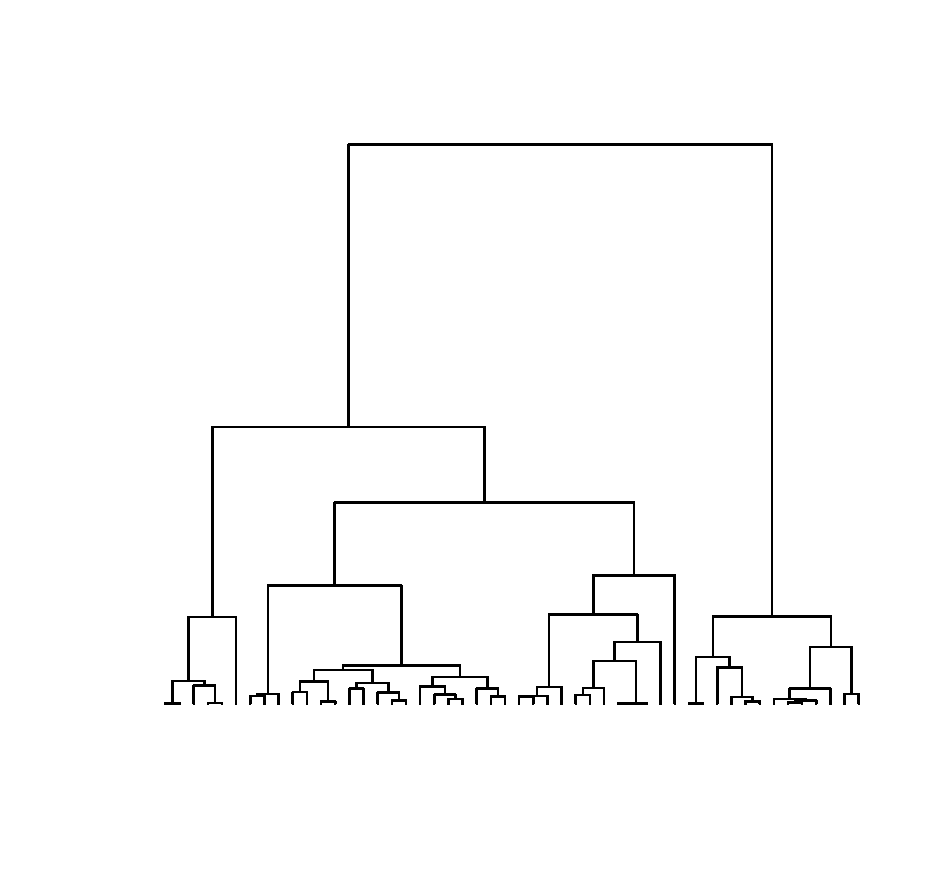
\includegraphics[width=0.6\textwidth, trim={2.8cm 3cm 1.5cm 2cm}, clip]{plots/ncoalescent.pdf}
\caption[The $n$-coalescent]{A realisation of the $n$-coalescent with $n=50$.}
\end{figure}
A particularly attractive feature of the $n$-coalescent is its tractability; its distribution and those of many statistics of interest are available in closed form (Section \ref{sec:KCproperties}).
It turns out also to be extremely useful as a limiting distribution in population genetics, including in its domain of attraction the genealogies of a wide range of population models (Section \ref{sec:popgenmodels}).


\subsection{Properties of Kingman's coalescent}\label{sec:KCproperties}
The simplicity of $Q$ allows various properties of the $n$-coalescent to be studied analytically.
Starting with $n$ blocks, exactly $n-1$ coalescences are required to reach the absorbing state where all blocks have coalesced, known in population genetics as the \emph{most recent common ancestor} (MRCA).

\begin{figure}[ht]
\centering
\begin{tikzpicture}
% horizontal lines
\draw[dotted, gray] (-0.5,-1)--(6,-1);
\draw[dotted, gray] (-0.5,-0.2)--(6,-0.2);
\draw[dotted, gray] (-0.5,0.5)--(6,0.5);
\draw[dotted, gray] (-0.5,1.3)--(6,1.3);
\draw[dotted, gray] (-0.5,3.3)--(6,3.3);

% tree
\draw[thick] (0,-1)--(0,-0.2);
\draw[thick] (1,-1)--(1,-0.2);
\draw[thick] (0,-0.2)--(1,-0.2);
\draw[thick] (0.5,-0.2)--(0.5,1.3);
\draw[thick] (2,-1)--(2,1.3);
\draw[thick] (0.5,1.3)--(2,1.3);
\draw[thick] (3,-1)--(3,0.5);
\draw[thick] (4,-1)--(4,0.5);
\draw[thick] (3,0.5)--(4,0.5);
\draw[thick] (1.25,1.3)--(1.25,3.3);
\draw[thick] (3.5,0.5)--(3.5,3.3);
\draw[thick] (1.25,3.3)--(3.5,3.3);

% interval arrows
\draw[<->] (5,-1)--(5,-0.2);
\draw[<->] (5,-0.2)--(5,0.5);
\draw[<->] (5,0.5)--(5,1.3);
\draw[<->] (5,1.3)--(5,3.3);

% small t's
\node at (5.2, -0.6) {\footnotesize{$t_5$}};
\node at (5.2, 0.15) {\footnotesize{$t_4$}};
\node at (5.2, 0.9) {\footnotesize{$t_3$}};
\node at (5.2, 2.3) {\footnotesize{$t_2$}};

% capital T's
\node[anchor=west] at (6, -1) {\footnotesize{$T_5 = 0$}};
\node[anchor=west] at (6, -0.2) {\footnotesize{$T_4$}};
\node[anchor=west] at (6, 0.5) {\footnotesize{$T_3$}};
\node[anchor=west] at (6, 1.3) {\footnotesize{$T_2$}};
\node[anchor=west] at (6, 3.3) {\footnotesize{$T_1 = T_{MRCA}$}};
\end{tikzpicture}
\caption{Definitions of $t_i$, $T_i$ in the $n$-coalescent.}
\label{fig:KC_timedefns}
\end{figure}

Denote by $t_2, \dots, t_n$ the waiting times between coalescent events, where $t_i$ is the amount of time for which the coalescent has exactly $i$ distinct lineages (see Figure~\ref{fig:KC_timedefns}).
A consequence of Definition~\ref{def:kingman} is that these waiting times are independent and have distributions
\begin{equation*}
t_i \sim \Exp\left( \binom{i}{2} \right) .
\end{equation*}
The partial sum $T_k := \sum_{i=k+1}^n t_i$ gives the total time up to the $(n-k)^{th}$ coalescence event, that is, the first time at which there are only $k$ lineages remaining out of the initial $n$ (see Figure~\ref{fig:KC_timedefns}).
The partial sums, being sums of independent Exponential random variables, have HypoExponential distributions.

Another important property of the $n$-coalescent is \emph{exchangeability}. That is, its law is invariant under permutations of the branches. This can be seen from \eqref{eq:KCgenerator} since the merge rate is equal for every pair of partitions $\xi \prec \eta$.
%\seb{Refer back to the following three properties later on with reference to their relevance in SMC.}

\subsubsection{Time to MRCA}
Of particular interest is the tree height or time to the most recent common ancestor, $T_{MRCA} := T_1$.
With some algebra we find, for instance,
\begin{equation*}
\E[ T_{MRCA} ] 
= \sum_{i=2}^{n} \E[t_i]
= \sum_{i=2}^n \frac{2}{i(i-1)}
= 2 \sum_{i=2}^n \left\{ \frac{1}{i-1} - \frac{1}{i} \right\}
= 2 \left( 1 - \frac{1}{n} \right)
\end{equation*}
and
\begin{equation*}
\V[ T_{MRCA} ] 
= \sum_{i=2}^n \V[t_i]
= \sum_{i=2}^n \left( \frac{2}{i(i-1)} \right)^2 .
\end{equation*}
The expected tree height converges to 2 as $n\to\infty$, and the variance converges to $4(\pi^2 - 9)/3 \simeq 1.16$.
The somewhat surprising fact that the tree height does not diverge with $n$ is a result of the very high rate of coalescence close to the bottom of the tree. This rate is large enough that the full Kingman coalescent (on $\mathbb{N}$) \emph{comes down from infinity}, that is, despite starting with infinitely many blocks, after any positive amount of time these have coalesced into finitely many blocks.
%\seb{Plot mean with sd-ribbon over $n$ for an illustration? SD ribbon isn't the right thing; since we apparently know the actual distribution, plot a high density interval of that. (also for $L$)}


\subsubsection{Total branch length}
Another quantity of interest is the total branch length,
$ L := \sum_{i=2}^n i t_i $.
For instance
\begin{equation*}
\E[ L ] 
= \sum_{i=2}^n i \E[ t_i ]
= \sum_{i=2}^n \frac{2}{i-1}
= \sum_{i=1}^{n-1} \frac{2}{i} %,
\simeq 2 \ln(n-1) 
\end{equation*}
%a harmonic series, 
and
\begin{equation*}
\V[ L ] 
= \sum_{i=2}^n i^2 \V[ t_i ]
= \sum_{i=2}^n \frac{4}{(i-1)^2}
= \sum_{i=1}^{n-1} \frac{4}{i^2} .
\end{equation*}
Note that although the mean total branch length diverges with $n$, the variance converges to a constant, $4\pi^2 /6 \simeq 6.58$.


\subsubsection{Probability that sample MRCA is population MRCA}
One other interesting quantity is the probability that the MRCA of $k$ random lineages coincides with the population MRCA \parencite[e.g.][Theorem 1.7]{durrett2008}.
Consider a random subsample of size $k$ among $n$ lineages distributed according to the $n$-coalescent.
Denote by $S_{k,n}$ the event that these $k$ lineages have the same MRCA as all $n$ lineages.
The probability of this event is calculated in \textcite[Example 1]{saunders1984} and again in \textcite[Equation (3)]{spouge2014}, in both cases arising as a special case of more general results. A direct proof is given below.
%Denote by $S_k$ the relevant event: that a random sample of size $k$ among $N$ lineages has the same MRCA as the population.

Consider the two subtrees produced by cutting the full population tree just below the population MRCA. The $k$ sampled lineages coalesce before the full-sample MRCA if and only if all $k$ sampled leaves lie in just one of these two subtrees.
Let $X$ be the number of leaves in the left subtree, so $X \in \{1,\dots,n-1\} $, and a consequence of the exchangeability of the $n$-coalescent is that $X$ is uniformly distributed on that set.
Conditional on $X$ we have
\begin{equation*}
\Prob [S_{k,n}^c \mid X=x]
= \left[ \binom{x}{k} + \binom{n-x}{k} \right] \binom{n}{k}^{-1} .
\end{equation*}
Integrating against the distribution of $X$ gives
\begin{align*}
\Prob[ S_{k,n} ]
&= 1 - \frac{1}{n-1} \binom{n}{k}^{-1} \, \sum_{x=1}^{n-1} 
        \left[ \binom{x}{k} + \binom{n-x}{k} \right] \\
&= 1 - \frac{1}{n-1} \binom{n}{k}^{-1} 
        \left[ \binom{n}{k+1} + \binom{n}{k+1} \right] \\
&= \frac{k-1}{k+1} \frac{n+1}{n-1}
\end{align*}
using binomial identities and some algebra.
In particular, when $k=2$ we have
\begin{equation*}
\Prob[ S_{2,n} ]
=\frac{n+1}{3(n-1)} 
\end{equation*}
as the probability that a randomly chosen pair of lineages does not coalesce until the MRCA of all $n$ lineages.
%, in the limit $N\to\infty$, the proportion of leaves in the left subtree is uniformly distributed on $[0,1]$.
%Calling this proportion $X$, we have
%\begin{equation*}
%\Prob [ S_k^c \mid X=x]
%= x^k + (1-x)^k
%\end{equation*}
%Integrating against the distribution of $X$, the probability of interest is
%\begin{equation*}
%\Prob[ S_k ]
%= 1- \int_0^1 [ x^k + (1-x)^k ] dx
%= \frac{k-1}{k+1}
%\end{equation*}
%as required.
%
%The above is based on properties of the full Kingman coalescent, but similar results are available for the $n$-coalescent.
%Consider now a subsample of size $k$ among $n$ lineages that follow the $n$-coalescent.
%Denote by $S_{k,n}$ the event that these $k$ lineages have the same MRCA as all $n$ lineages.
%This probability of this event is calculated in \textcite[Example 1]{saunders1984} and again in \textcite[Equation (3)]{spouge2014}, in both cases arising as a special case of more general results. A direct proof is given below.
%
%Let $X$ be the number of leaves in the left subtree. So $X \in \{1,\dots,n-1\} $ and, like before, a consequence of exchangeability is that $X$ is uniformly distributed on that set.
%Now that the total number of branches is finite, we have to count more carefully. 
%As $n\to\infty$ this agrees with the population-level result above.



\subsection{Models in population genetics}\label{sec:popgenmodels}
The Kingman coalescent is the limiting coalescent process (in the large population limit) for a surprisingly wide range of population models. Some important examples of models in this ``domain of attraction'' are introduced in this section.
Common to all of these models are the following assumptions:
\begin{itemize}
\item The population has constant size $N$
\item Reproduction happens in discrete generations
\item The mechanism for assigning offspring to parents is identical at each generation, and independent between generations
\item The offspring distribution is exchangeable.
\end{itemize}
As in Section~\ref{sec:SMC_FK}, we define offspring counts in terms of parental indices as $\nu_j := |\{ i: a_i = j\}|$.
Since the assignment of offsrping to parents is i.i.d.\ across generations, there is no dependence on $t$.
Also, under the assumption of exchangeability, it is sufficient to consider only the offspring counts, rather than the parental indices (which generally carry more information).
%\seb{Crucially, in the neutral case, offspring counts carry all the information about the distribution of the genealogy that is contained in the parental indices.}
These models are all \emph{neutral}, that is exhibiting no natural selection, because the offspring counts at each generation are independent, so there can be no preferential propagation of certain ``fitter'' lineages.




\subsubsection{Cannings model}
The neutral Cannings model \parencite{cannings1974, cannings1975} is a general class which encompasses some other important models as special cases.

The Cannings model does not specify a particular distribution for the offspring counts; it just requires that the distribution is exchangeable, i.i.d.\ between generations, and preserves the population size. In particular, the probability of observing offspring counts $(v_1, \dots, v_N)$ must be invariant under permutations of this vector.

Rescaled genealogies of the neutral Cannings model converge to the Kingman coalescent as $N\to\infty$, under some conditions on the moments of the offspring distribution. 
For example, one may apply the sufficient conditions of \textcite{kingman1982gene}:
if $\V[\nu_1] \to \sigma^2 \in (0,\infty)$ and $\E[\nu_1^k]$ is bounded for all $k\in\mathbb{N}$ then, under the time scaling $N\sigma^{-2}$, the genealogies of the neutral Cannings model converge to the Kingman coalescent.
%\parencite[see for example][Section 2.2]{etheridge2011}. \seb{original reference for this? is not any Kingman 1982 papers, and certainly not Cannings 1974/5 which predates KC}




\subsubsection{Wright-Fisher model}
The neutral Wright-Fisher model \parencite{fisher1923, fisher1930, wright1931} is one of the most studied models in population genetics.
At each generation the existing population dies and is replaced by $N$ offspring. The offspring descend from parents $(a_1, \dots, a_N)$ which are selected according to
\begin{equation*}
a_i \overset{iid}{\sim} \Cat(\{1, \dots, N\}, (1/N, \dots, 1/N)).
\end{equation*}
The joint distribution of the offspring counts is therefore
\begin{equation*}
(v_1,\dots, v_N) \sim \Mn(N, (1/N, \dots, 1/N)).
\end{equation*}
Since the Multinomial distribution is exchangeable, the Wright-Fisher model is a special case of the Cannings model.
%There are several non-neutral variants of the Wright-Fisher model \seb{citations?}, but they are typically much less tractable than the neutral one.

\textcite{kingman1982gene} showed that the Wright-Fisher model satisfies his sufficient conditions, and thus the resulting genealogies, appropriately rescaled, converge to the Kingman coalescent as $N\to\infty$.
The correct time scale in this instance is $N$, since
\begin{equation*}
\V[\nu_1] = N\frac{1}{N} \left
(1 - \frac{1}{N}\right)
=\frac{N-1}{N}
\to 1 
=: \sigma^2 ,
\end{equation*}
so $N\sigma^{-2} = N$.



\subsubsection{Moran model}
The neutral Moran model \parencite{moran1958}, while perhaps less biologically relevant, is mathematically appealing because its simple dynamics make it particularly tractable.

At each generation, an ordered pair of individuals is selected uniformly at random. The first individual in this pair dies (i.e.\ leaves no offspring in the next generation), while the other reproduces (leaving two offspring). All of the other individuals leave exactly one offspring.
This is another special case of the neutral Cannings model, where the offspring distribution is now uniform over all permutations of $(0,2,1,1,\dots,1)$.

Under a suitable time-scaling, its genealogies converge to the Kingman coalescent,
%\seb{[citation]}
although the sufficient conditions of \textcite{kingman1982gene} do not apply:
\begin{align*}
\V[\nu_1] 
&= \E[\nu_1^2] - \E[\nu_1]^2
= (0 + 1 \cdot \frac{N-2}{N} + 4 \cdot \frac{1}{N}) - (0 + 1 \cdot \frac{N-2}{N} + 2 \cdot \frac{1}{N})^2 \\
&= \frac{N+2}{N} - 1^2
= \frac{2}{N}
\to 0 ,
\end{align*}
violating the condition that $\sigma^2 >0$. 
That condition turns out not to be necessary, and $\V[\nu_1]$ gives us the correct time scale on which to recover the Kingman coalescent: $N(\V[\nu_1])^{-1} = N^2/2$.
It is not surprising that the time scale is an order bigger than in the Wright-Fisher model, because the Moran model has a reproduction rate $O(N)$ times lower than in the Wright-Fisher model: at each generation $2$ individuals are involved in reproduction, as opposed to $N$ in the Wright-Fisher model.
%\seb{also cite a Moran-specific convergence result: not sure where (it isn't in Kingman 1982* or in Moran 1958 which predates KC)}




\subsection{Other convergence results}
\label{sec:previousgeneconv}
The original work of \textcite{kingman1982gene} provides sufficient conditions for the finite-dim\-ension\-al distributions of genealogies of Cannings models to converge to those of the Kingman coalescent.
\textcite{mohle1998} provides another set of sufficient conditions which apply to the wider class of models in which the population size may vary deterministically, the offspring distributions are independent but not identical across generations, and exchangeability is replaced by the weaker \emph{random assignment} condition. 
For that class of models under the same conditions, \textcite{mohle1999} proves that the genealogies converge weakly as well as in the sense of finite-dimensional distributions.
\textcite{mohle2000} gives a simpler condition which is necessary and sufficient for convergence of Cannings genealogies to the Kingman coalescent. % that N&S condition is the exchangeable version of our main theorem condition.

Meanwhile many similar results were established for models in which the limiting process is not the Kingman coalescent.
Relaxing the conditions to allow multiple mergers in the limit admits $\Lambda$-coalescents as limiting processes, with the Kingman coalescent as a special case \parencite{pitman1999, sagitov1999, mohlesagitov1998}.
If simultaneous mergers are also allowed, the limiting process belongs to the even more general class of $\Xi$-coalescents \parencite{mohle2001}, and this class encompasses all possible limiting genealogies of Cannings models.
On the other hand, \textcite{delmoral2009} do not consider asymptotics in the population size, but instead prove some properties of neutral models with fixed population $N$, particularly concerning the MRCA. 

The focus of the current work is on systems that admit Kingman genealogies in the limit, among a wider class of models where, like \textcite{mohle1998, mohle1999}, exchangeability is relaxed to random assignment, and we also do not require independence between generations, so our models are not neutral. 
%In particular, this class of models is non-neutral.
Our main condition for convergence to the Kingman coalescent, which is introduced in Chapter~\ref{ch:limits}, can be considered a non-exchangeable non-neutral analogue of the condition presented in \textcite{mohle2000}.




\subsection{Particle populations}
Much of the population genetics framework transfers readily to the case of SMC. The population is now a population of particles, with each iteration of the SMC algorithm corresponding to a generation, and resampling playing the part of reproduction.
In fact, SMC populations are in some ways more suited to these population models than actual biological populations.
For example, the assumptions that the population has constant size $N$ and that reproduction occurs only at discrete generations are satisfied by construction.

However, we cannot assume independence between generations: as seen in Figure~\ref{fig:cond_indep_graph}, the offspring counts at subsequent iterations of an SMC algorithm are not independent without some conditioning. 
This means that SMC populations are not neutral.
In fact, after marginalising out the information about the positions of the particles, the genealogical process is not even Markovian.





\section{Sequential Monte Carlo genealogies}
\label{sec:SMC_genealogies}
%\subsection{From particles to genealogies}
We have seen that genetic terminology applies quite naturally to SMC.
The resampling step induces parent-offspring relationships, each duplicate of particle $i$ after resampling being considered one of its offspring. Then follows the notion of offspring counts (also known as family sizes), that is, the number of offspring assigned to each parent.
Viewed backwards in time, the parent-offspring relationships also imply a genealogy, obtained by tracing the lineages from each terminal particle through its ancestor in each generation.
We will see in this section that these genealogies, induced by resampling, are not a mere curiosity but in fact have important implications for the performance of SMC algorithms.




\subsection{Ancestral degeneracy}
\label{sec:anc_degen}
Suppose we were using SMC to sample from the smoothing distribution of some state space model.
As described in Section~\ref{sec:SMC_FK}, we run our chosen SMC algorithm forwards, then output the $N$ sampled trajectories $X_{t,0:t}^{(i)}$ (for each $i\in\{1,\dots,N\}$).
Each trajectory was obtained by tracing back through the parent at each generation, starting from one of the terminal particles. 
This means that if two terminal particles $i$ and $j$ share a common ancestor at some generation $s$, then $X_{t,0:s}^{(i)}$ will be exactly equal to $X_{t,0:s}^{(j)}$, because their ancestries coincide from time $s$ to $0$.

At every resampling step, some parents may be assigned more than one offspring each, so the further back in time you look, the more of the ancestries of the terminal particles will have coalesced (see Figure~\ref{fig:ancdegen_mn}).
The effect of this is that, instead of obtaining $N$ separate sampled trajectories, we actually obtain $N$ sampled trajectories that coalesce backwards in time, which means that the further back in time we look, the fewer distinct samples we have from the corresponding component of the target distribution.
Particularly if we are interested in smoothing over a long time horizon, the variance of the SMC estimator is going to blow up.

\begin{figure}[ht]
\centering
\subfloat[Multinomial resampling]{
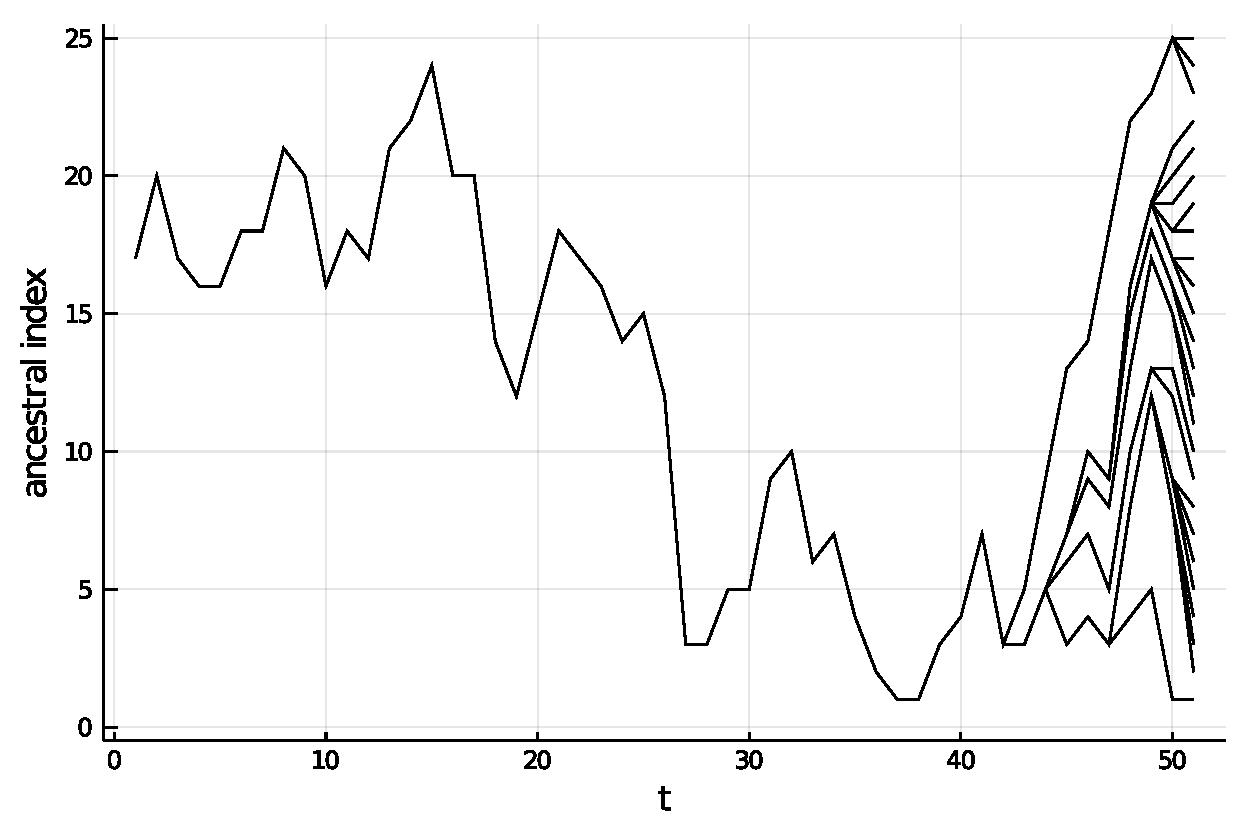
\includegraphics[width=0.47\textwidth]{plots/ancdegen_mn.pdf}
\label{fig:ancdegen_mn}
}
\subfloat[Adaptive minimum-variance resampling]{
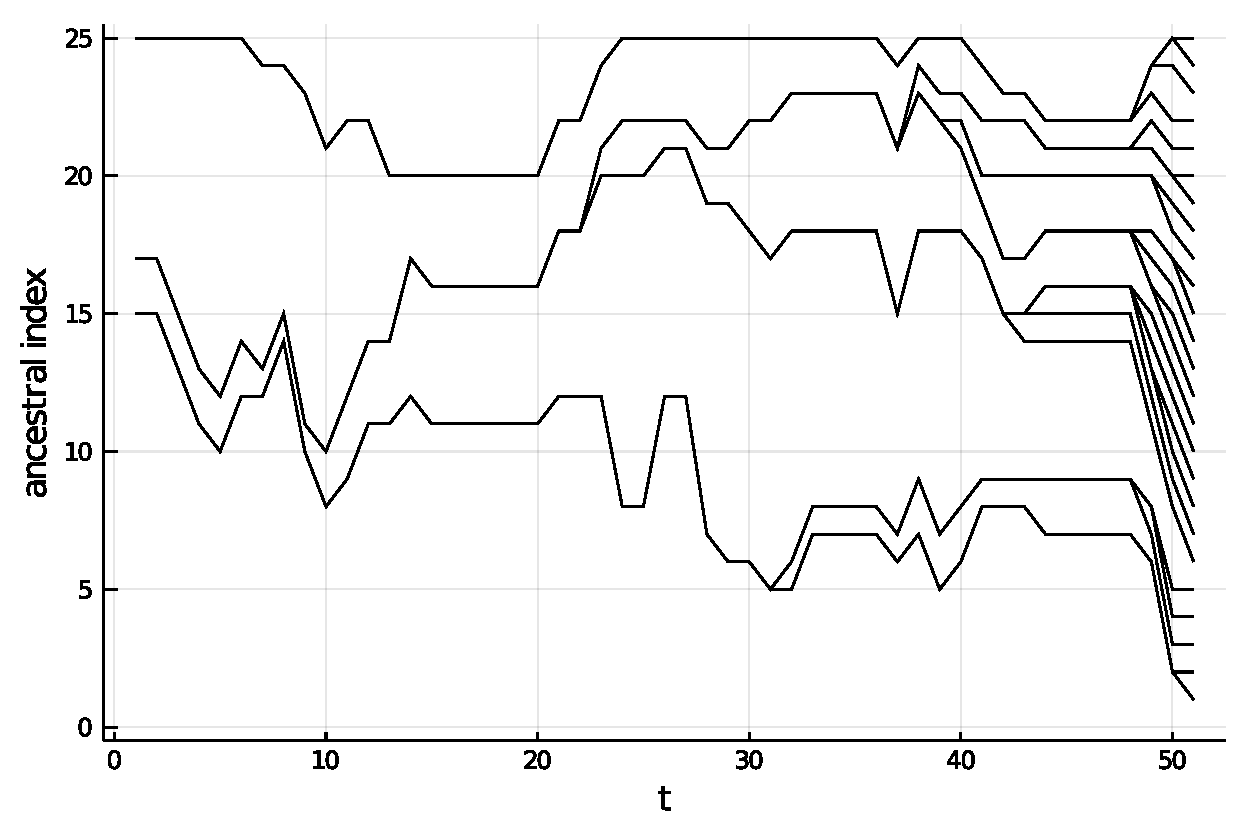
\includegraphics[width=0.47\textwidth]{plots/ancdegen_adaptsyst.pdf}
\label{fig:ancdegen_adaptsyst}
}
\caption[Ancestral degeneracy]{Illustration of ancestral degeneracy and the mitigating effect of low-variance and adpative resampling.
Each line is the lineage of one of the terminal particles, indicating the index of its ancestor in each generation:
\subref{fig:ancdegen_mn} with multinomial resampling;
\subref{fig:ancdegen_adaptsyst} the same system with adaptive systematic resampling.}
\label{fig:ancestral_degeneracy}
\end{figure}
On the other hand, ancestral degeneracy actually improves the memory efficiency of SMC. We do not need to store all of the particles generated at each time (at memory cost $O(NT)$), only those that are included in the resulting genealogy. \textcite{jacob2015} provide an algorithm for efficient storage of the genealogy, reducing the asymptotic memory cost to $O(N\log N+T)$.
However, it is certainly still worth trying to reduce ancestral degeneracy because to achieve a given level of error with a highly degenerate system will require such a large $N$ that any such memory gains are cancelled out.
%(a) because computation is often the limiting factor rather than memory, and (b) 


\subsubsection{Mitigating ancestral degeneracy}
There are a few possible approaches to mitigating ancestral degeneracy.
Firstly, we could try to limit the number of offspring assigned to any one parent during each resampling step. We can only go so far, because we need the resampling procedure to remain unbiased (as discussed in Section~\ref{sec:SMC_FK}), but we can try to reduce the variance inherent in the resampling procedure. This idea, known as \emph{low-variance resampling} is explored in detail in Section~\ref{sec:resampling}.

Another idea is to resample less often. Recall that the reason for resampling is to prevent weight degeneracy (that is, one of the weights tending to one while the others tend to zero). Now we see that, while solving one type of degeneracy, resampling creates another. The effect of ancestral degeneracy is essentially the same as that of weight degeneracy: both drastically increase the variance of the resulting SMC estimators. 
We can therefore consider a trade-off between the two, which is the idea behind \emph{adaptive resampling} \parencite[Section 4]{liu1995}.
The trick is to apply the resampling step only at iterations in which a certain criterion is met. The most commonly-used criterion, suggested by \textcite[Equation (14)]{liu1995}, is based on the \emph{effective sample size}
\begin{equation*}
ESS(t) := \left\{ \sum_{i=1}^N (w_t^{(i)})^2 \right\}^{-1} ,
\end{equation*}
which decreases as the weights degenerate.
The resampling step is then applied only at iterations $t$ such that $ESS(t)$ is less than some pre-specified threshold, typically $N/2$. %\seb{[citation?]}

If adaptive resampling is used, some trivial changes are required to the calculation of the weights in Algorithm~\ref{alg:SMC}, to allow for the importance weights to accumulate sequentially until the particles are resampled. See e.g.\ \textcite[Section 10.2]{chopin2020} for details.

As well as mitigating ancestral degeneracy, adaptive resampling has the virtue of saving some computation (although the overall asymptotic complexity of the SMC algorithm does not change).
How effective adaptive resampling will be depends on the particular application and choice of SMC algorithm. If the proposals (i.e.\ transition kernels) are not very close to their targets then the weights will degenerate rapidly and the effective sample size criterion (or similar) will not reduce the frequency of resampling very much.

Low-variance resampling is also less effective under poor proposals: the resulting high-variance weights lead to high-variance offspring counts, even under minimum-variance resmapling schemes, because the resampling is required to be unbiased.

Adaptive resampling and low-variance resampling can be combined, and this is widely considered to be the best practice when implementing SMC.
Figure~\ref{fig:ancestral_degeneracy} compares ancestral degeneration under multinomial resampling (a relatively high variance scheme) to the same under adaptive resampling with a minimum-variance resampling scheme.
It is clear that the degeneration is much more severe in the former case.

There is one technique that completely solves the problem of ancestral degeneracy, namely \emph{backward simulation} \parencite{godsill2004}. This involves running an SMC algorithm as usual (the \emph{forward pass}), and then sampling new ancestors for each particle during an additional \emph{backward pass}. 
The backward-simulated parents in each generation are chosen among all $N$ particles, making use of particles that were not included in the forward-sampled trajectories.
The effect on genealogies is striking: the lineages are now sampled independently, so the coalescences caused by resampling do not feature at all in the output genealogies.

Since this work concerns genealogies induced by resampling, we will not say much more about backward simulation. There are many situations in which it is impossible to implement and therefore the study of SMC genealogies is still of interest. 
Firstly, backward simulation inherently requires a forward and backward pass through all of the data, so it cannot be implemented on-line. 
Secondly, calculating the backward-simulation probabilities requires the Markov kernels $M_t$ of the corresponding Feynman-Kac model to admit densities that can be evaluated pointwise. This is much stronger than the ability to simulate from $M_t$, the requirement for applying standard SMC algorithms.




\subsection{Asymptotic genealogies}
If we had access to information about the behaviour of SMC genealogies a priori (i.e.\ without having run the algorithm), we would be in a position to answer many questions of interest. These include practical questions about tuning, for example:
\begin{itemize}
\item How many particles should I use in order to maintain (with high enough probability) a given level of error over a time horizon $T$?
\item With $N$ particles, what is the largest lag over which fixed-lag smoothing produces reasonable estimates?
\item How many particles should I use within particle Gibbs to ensure that (with high enough probability) at least two distinct trajectories survive each iteration?
\end{itemize}
This last question touches on a critical aspect of the performance of particle Gibbs algorithms, which is discussed in Section~\ref{sec:condSMC}.
We could also consider theoretical questions, such as:
\begin{itemize}
\item For a given class of models and algorithms, what is the effect of ancestral degeneracy on how the estimators behave over time?
\item Which resampling schemes lead to the smallest amount of ancestral degeneracy?
\item What is the effect on genealogies of adaptive resampling?
\end{itemize}
Many of these questions have already been partially addressed, without any explicit analysis of genealogies, by way of variance calculations and simulation experiments.
But since these are all genealogical questions by nature, it seems sensible to work directly with the genealogies, if possible.
The problem is that the genealogy of particles is a complex object, it is random, and it can depend strongly on the particular choice of Feynman-Kac model and SMC implementation.

It turns out that these problems can be somewhat overcome by considering the genealogies in an asymptotic regime where the number of particles $N$ tends to infinity.
In this regime, many different particle systems exhibit genealogies of a common form, namely Kingman's $n$-coalescent under suitable time-scalings. The genealogical differences between various algorithms is then encoded by their respective time-scale functions. This is still a random object but is less complicated than the genealogy itself; namely a c\`adl\`ag function as opposed to a labelled weighted tree.

In the context of SMC, these asymptotic genealogies were first analysed by \textcite{koskela2018}. The simulations therein suggest that such asymptotic results also transfer to finite systems, making them practically useful.
One of the contributions of the current work is to demonstrate that Kingman-type genealogies arise from a wide variety of SMC algorithms, including those most commonly used in practice.
In principle this means, for instance, that genealogies of different SMC algorithms can be compared by examining the corresponding time-scale functions.





\section{Resampling}
\label{sec:resampling}
As we have seen, resampling is necessary within SMC to ``reset'' the weights in order to prevent weight degeneracy.
Resampling is itself a Monte Carlo procedure: the discrete offspring counts can be viewed as stochastic estimates of the continuous weights.
In order to obtain a valid SMC algorithm, these Monte Carlo samples must be unbiased; this and other desirable properties are formalised in Definition~\ref{defn:resampling}.
There is a huge range of resampling procedures satisfying these properties, some of which perform better than others. 
Some of the most popular resampling schemes are introduced in Section~\ref{sec:examples_resamplingschemes} and their properties are explored in Section~\ref{sec:resampling_properties}.




\subsection{Definition}

\begin{defn}\label{defn:resampling}
For our purposes, a valid resampling scheme is a stochastic function mapping weights 
$w_t^{(1:N)} \in \mathcal{S}_{N-1}$ 
to offspring counts 
$\nu_t^{(1:N)} \in \{0,\dots,N\}^N $
that satisfies the following conditions:
\begin{enumerate}
\item\label{item:resampling_property1} the population size is conserved:
$ \sum_{i=1}^N \nu_t^{(i)} =N $
\item\label{item:resampling_property2} the weights are equal after resampling:
$w_{t+}^{(i)} = 1/N$ for all $i$
\item\label{item:resampling_property3} the resampling is unbiased:
$ \E[ \nu_t^{(i)} \mid w_t^{(i)} ] = N w_t^{(i)} $ for all $i$.
\end{enumerate}
\end{defn}
It is possible to design resampling schemes that violate these properties.
Resampling different numbers of particles in different iterations (violating condition \ref{item:resampling_property1}) is of course possible \parencite[see for example][]{crisan1998}, but we typically have a fixed limit on computational resources, so in most cases it makes sense to simulate the maximum feasible number of particles $N$ at every iteration.
There may be circumstances under which it is beneficial to allow the number of particles to vary adaptively \parencite{fox2003,chau2012,lee2018} or at random, but this is not commonly done in practice.

Condition \ref{item:resampling_property2} is sensible because the whole point of resampling is to reset the weights. However, there are several examples in the literature where the weights are only ``partially'' reset, so that the variance of weights after resampling is not zero, but is lower than before resampling.
For example, a scheme of \textcite{liu1998} uses the square roots of the weights for resampling, then corrects by setting unequal weights after resampling (violating conditions \ref{item:resampling_property2} and \ref{item:resampling_property3}).
\textcite[Section 3.1]{liu2001} generalise this further, and suggest setting the resampling weights adaptively as a function of the true weights $w_t^{(1:N)}$.
\textcite{fearnhead2003} present an optimal resampling scheme in the case that the state space is discrete, which similarly uses weights other than $w_t^{(1:N)}$ for resampling and corrects by giving the particles unequal weights after resampling.
The \emph{chopthin} resampling algorithm of \textcite{gandy2016} also violates condition \ref{item:resampling_property2}.

Deterministic resampling schemes (which cannot generally be unbiased, violating condition \ref{item:resampling_property3}) have been used by some authors. One such scheme was proposed by \textcite{kitagawa1996} but is now generally implemented only in its randomised form (see \emph{systematic resampling} below). More recent examples include schemes based on optimal transport \parencite{reich2013, myers2021, corenflos2021} and the \emph{importance support points} resampling of \textcite{huang2020}.

The mutation and weighting steps of SMC are embarrassingly parallel, but resampling is not easy to parallelise, presenting a bottleneck to running SMC on parallel or distributed computer architectures. %There has therefore been a lot of interest recently in parallelising the resampling step.
\textcite{whiteley2016} show that it is possible to construct resampling schemes that perform well whilst only requiring interaction of a few particles at a time, suggesting that parallel resampling is possible, and further details concerning implementation are provided in \textcite{lee2016}.
The \emph{Metropolis resampler} of \textcite{murray2016} resamples in parallel via a Metropolis MCMC algorithm, but this introduces bias and thus violates condition \ref{item:resampling_property3}. 
\textcite{murray2016} also propose \emph{rejection resampling}, which is unbiased. This constitutes an alternative method for \emph{multinomial resampling} (see below) which offers speed-ups when computing in parallel but requires that an upper bound on the weights is known.
A variant that only requires an ``approximate'' upper bound on the weights is also presented, but this does not use the true weights for resampling, and so violates conditions \ref{item:resampling_property2} and \ref{item:resampling_property3}.

The majority of resampling schemes in the literature fit within Definition~\ref{defn:resampling}, and it is not usually advantageous to violate the properties \ref{item:resampling_property1}--\ref{item:resampling_property3}.
Definition~\ref{defn:resampling} still allows a great deal of flexibility in the choice of resampling scheme, and many such schemes have been proposed, some performing better than others. 
Some important resampling schemes are reviewed in Section~\ref{sec:examples_resamplingschemes}, and their performance is discussed in detail in Section~\ref{sec:resampling_properties} and summarised in Table~\ref{tab:resampling_properties}.




\subsection{Examples}
\label{sec:examples_resamplingschemes}

 
\subsubsection{Multinomial resampling}
%\label{sec:resampling_multinomial}
%\draft{Remark that this is similar to Wright-Fisher model (Section~\ref{sec:popgenmodels}), but with random non-uniform weights that are dependent over time...?}\\
Multinomial resampling \parencite{rubin1987,gordon1993,efron1994} is one of the simplest resampling schemes.
The parental indices are chosen independently from $\{1, \dots, N\}$, each with probability given by the weight of the corresponding particle $w_t^{(i)}$. 
That is, 
\begin{equation*}
a_t^{(1:N)} \simiid \Cat( \{1,\dots, N\}, w_t^{(1:N)} ) .
\end{equation*}
This implies that the joint distribution of the offspring counts is 
\begin{equation*}
\nu_t^{(1:N)} \eqdist \operatorname{Multinomial}(N, w_t^{(1:N)} ) .
\end{equation*}
It follows from properties of the Multinomial distribution that this resampling scheme is unbiased.
%\seb{Although the parental indices are chosen independently, the resulting offspring counts are negatively correlated. --- link to GCW19's negative association?}

A simple way to sample the parental indices is to use inversion sampling: partition the unit interval into $N$ subintervals each of which will correspond to a certain index $i$ and has length equal to the weight $w_t^{(i)}$; then draw $N$ samples $U_i \sim \Unif[0,1]$ and classify them according to which of these subintervals they fall in.
Explicitly, the parental index assigned to child $i$ is the index $a_i$ satisfying
\begin{equation}\label{eq:syst_strat_resampling}
\sum_{j=1}^{a_i -1} w_t^{(j)} \leq U_i \leq \sum_{j=1}^{a_i} w_t^{(j)} .
\end{equation}
This is illustrated in Figure \ref{fig:inv_resampling}. 
%Note that there exist more efficient methods to sample from a Multinomial distribution, so the inversion method may not be used in practice.

Fast implementations of multinomial resampling rely on $U_1,\dots,U_N$ being pre-sorted, which speeds up the search step \eqref{eq:syst_strat_resampling}. Sorting $N$ numbers requires $O(N\log N)$ computation, but this is not necessary since we can sample directly the order statistics of a $\Unif[0,1]$ distribution, at $O(N)$ cost.
This can be done either by 
sampling $X_i \sim \Exp(1)$ independently for $i=1,\dots,N+1$ and outputting the normalised sums
\begin{equation*}
U_k := \frac{\sum_{i=1}^k X_i}{\sum_{i=1}^{N+1} X_i}
\end{equation*}
for $k=1,\dots,N$,
or by sampling $X_i \sim \Unif[0,1]$ independently for $i=1,\dots,N$ and computing recursively
\begin{equation*}
U_N := X_N^{1/N} , \qquad U_k := X_k^{1/k} U_{k+1} ;
\end{equation*}
see \textcite[Chapter 5, Section 3.1]{devroye1986}.
%One way to do this \parencite[Proposition 9.1]{chopin2020} is to sample $X_i \sim \Exp(1)$ independently for $i=1,\dots,N+1$ and output the normalised sums
%\begin{equation*}
%U_k := \frac{\sum_{i=1}^k X_i}{\sum_{i=1}^{N+1} X_i}
%\end{equation*}
%for $k=1,\dots,N$.
%Another method \parencite{hol2006} is to sample $X_i \sim \Unif[0,1]$ for $i=1,\dots,N$ and compute recursively
%\begin{equation*}
%U_N := X_N^{1/N} , \qquad U_k := X_k^{1/k} U_{k+1} .
%\end{equation*}
This allows multinomial resampling to be implemented at $O(N)$ cost. 
A side-effect is that the sampled ancestral indices will be ordered and therefore cannot be Categorically distributed, although the offspring counts still have the correct Multinomial distribution. For the purposes of resampling this isn't usually a problem, but the Categorical distribution can anyway be restored at $O(N)$ cost by applying a random permutation to the offspring indices.




\subsubsection{Residual resampling}
%\label{sec:resampling_residual}
Residual resampling is described in \textcite{liu1998} and also in \textcite{whitley1994} where it is called ``remainder stochastic sampling''.

Each particle $X_{t}^{(i)}$ is deterministically assigned $\flnw$ offspring, and the remaining
\begin{equation*}
R := \sum_{i=1}^N ( Nw_t^{(i)} - \flnw) = N- \sum_{i=1}^N \flnw
\end{equation*}
offspring are assigned stochastically according to the residual weights
\begin{equation*}
r^{(i)} := ( Nw_t^{(i)} - \flnw) /R .
\end{equation*}
Notice that each $r^{(i)}$ lies in the interval $[0, 1/R)$, and $R\in\{0,\dots,N-1\}$ with $R=0$ only if all weights are multiples of $1/N$ in which case all residual weights are zero.

The stochastic part can be implemented using any of the other basic resampling schemes (e.g.\ multinomial, stratified, systematic). Most presentations focus on the case where multinomial resampling is used for the residuals, which is by no means the most sensible choice. We will explore several different options in what follows.

%This yields a vector of offspring counts
%\begin{equation*}
%\nu_t^{(1:N)} \eqdist \lfloor N w_t^{(1:N)} \rfloor +  \operatorname{Multinomial}(R, (N w_t^{(1:N)} - \lfloor N w_t^{(1:N)}\rfloor)/R) .
%\end{equation*}
%The deterministic part ensures that every particle with weight $>1/N$ is guaranteed to survive. This is a desirable property as it prevents the random loss of high-weighted particles.

\begin{figure}
\centering
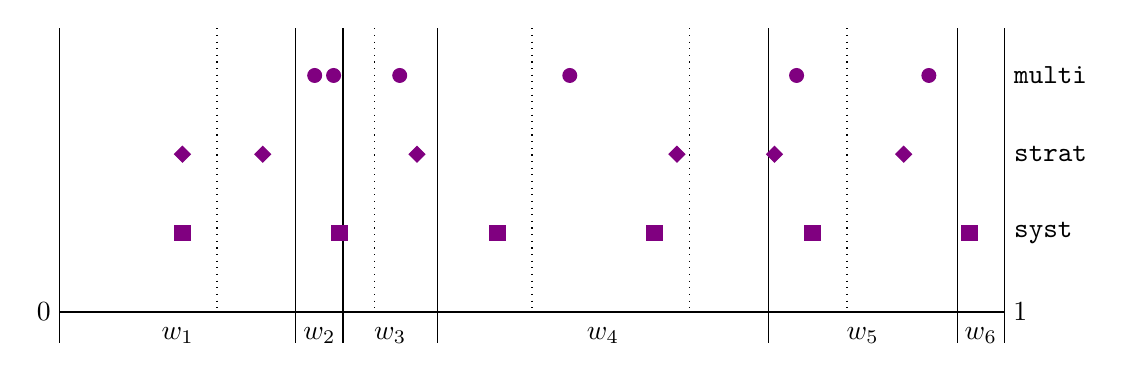
\begin{tikzpicture}
%% w = (0.25, 0.05, 0.10, 0.35, 0.20, 0.05)
%% u = (0.78, 0.29, 0.27, 0.92, 0.54, 0.36)
%%parallel lines
\draw[thick] (0,1) -- (12,1);
%\draw (0,2) -- (12,2);
%\draw (0,3) -- (12,3);
%\draw (0,4) -- (12,4);
%% endpoint labels
\node at (-0.2,1) {$0$};
\node at (12.2,1) {$1$};
%% vertical lines indicating weight intervals
\draw (0,4.6) --(0,0.6);
\draw (3,4.6) --(3,0.6);
\draw (3.6,4.6) --(3.6,0.6);
\draw (4.8,4.6) --(4.8,0.6);
\draw (9,4.6) --(9,0.6);
\draw (11.4,4.6) --(11.4,0.6);
\draw (12,4.6) --(12,0.6);
%% weight labels
\node at (1.5,0.7) {$w_1$};
\node at (3.3,0.7) {$w_2$};
\node at (4.2,0.7) {$w_3$};
\node at (6.9,0.7) {$w_4$};
\node at (10.2,0.7) {$w_5$};
\node at (11.7,0.7) {$w_6$};
%% vertical lines spaced 1/N apart
\draw[dotted] (2,4.6) --(2,1);
\draw[dotted] (4,4.6) --(4,1);
\draw[dotted] (6,4.6) --(6,1);
\draw[dotted] (8,4.6) --(8,1);
\draw[dotted] (10,4.6) --(10,1);
%% resampling scheme labels
\node[anchor=west] at (12,4) {\texttt{multi}};
\node[anchor=west] at (12,3) {\texttt{strat}};
\node[anchor=west] at (12,2) {\texttt{syst}};
%% multinomial points (top row)
\filldraw[violet] (9.36,4) circle (2.5pt);
%\node[anchor=south, violet] at (9.36,4) {$u_1$};
\filldraw[violet] (3.48,4) circle (2.5pt);
%\node[anchor=south, violet] at (3.54,4) {$u_2$};
\filldraw[violet] (3.24,4) circle (2.5pt);
%\node[anchor=south, violet] at (3.18,4) {$u_3$};
\filldraw[violet] (11.04,4) circle (2.5pt);
%\node[anchor=south, violet] at (11.04,4) {$u_4$};
\filldraw[violet] (6.48,4) circle (2.5pt);
%\node[anchor=south, violet] at (6.48,4) {$u_5$};
\filldraw[violet] (4.32,4) circle (2.5pt);
%\node[anchor=south, violet] at (4.32,4) {$u_6$};
%% stratified points (middle row)
\filldraw[violet] (1.46,3)--(1.56,3.1)--(1.66,3)--(1.56,2.9)--cycle;
%\node[anchor=south, violet] at (1.56,3) {$u_1$};
\filldraw[violet] (2.48,3)--(2.58,3.1)--(2.68,3)--(2.58,2.9)--cycle;
%\node[anchor=south, violet] at (2.58,3) {$u_2$};
\filldraw[violet] (4.44,3)--(4.54,3.1)--(4.64,3)--(4.54,2.9)--cycle;
%\node[anchor=south, violet] at (4.54,3) {$u_3$};
\filldraw[violet] (7.74,3)--(7.84,3.1)--(7.94,3)--(7.84,2.9)--cycle;
%\node[anchor=south, violet] at (7.84,3) {$u_4$};
\filldraw[violet] (8.98,3)--(9.08,3.1)--(9.18,3)--(9.08,2.9)--cycle;
%\node[anchor=south, violet] at (9.12,3) {$u_5$};
\filldraw[violet] (10.62,3)--(10.72,3.1)--(10.82,3)--(10.72,2.9)--cycle;
%\node[anchor=south, violet] at (10.72,3) {$u_6$};
%% systematic points (bottom row)
\filldraw[violet] (1.46,1.9)--(1.46,2.1)--(1.66,2.1)--(1.66,1.9)--cycle;
%\node[anchor=south, violet] at (1.56,2) {$u_1$};
\filldraw[violet] (3.46,1.9)--(3.46,2.1)--(3.66,2.1)--(3.66,1.9)--cycle;
%\node[anchor=south, violet] at (3.56,2) {$u_2$};
\filldraw[violet] (5.46,1.9)--(5.46,2.1)--(5.66,2.1)--(5.66,1.9)--cycle;
%\node[anchor=south, violet] at (5.56,2) {$u_3$};
\filldraw[violet] (7.46,1.9)--(7.46,2.1)--(7.66,2.1)--(7.66,1.9)--cycle;
%\node[anchor=south, violet] at (7.56,2) {$u_4$};
\filldraw[violet] (9.46,1.9)--(9.46,2.1)--(9.66,2.1)--(9.66,1.9)--cycle;
%\node[anchor=south, violet] at (9.56,2) {$u_5$};
\filldraw[violet] (11.46,1.9)--(11.46,2.1)--(11.66,2.1)--(11.66,1.9)--cycle;
%\node[anchor=south, violet] at (11.56,2) {$u_6$};
\end{tikzpicture}
\caption[Inversion sampling for multinomial, stratified and systematic resampling]{Inversion sampling interpretation of multinomial, stratified and systematic resampling.
In this example, $N=6$, $w^{(1:6)} = (0.25,0.05,0.1,0.35,0.2,0.05)$ and the uniform random variables input to the resampling schemes are $u_{1:6} = (0.78, 0.29, 0.27, 0.92, 0.54, 0.36)$.
The solid vertical lines show the partition of $[0,1]$ into subintervals with lengths $w^{(1:6)}$.
The dotted vertical lines show the partition of $[0,1]$ into subintervals of length $1/N$, used for stratified and systematic resampling.\\
Top row (circles): in multinomial resampling, $u_{1:6}$ are fed directly into the inversion sampler. Which subinterval $u_i$ falls into determines the parent of offspring $i$. The resulting offspring counts in this example are $\nu^{(1:6)} = (0,2,1,1,2,0)$.\\
Middle row (diamonds): in stratified resampling, $u_{1:6}$ are transformed so that one point lies in each subinterval of length $1/N$. The resulting offspring counts are $\nu^{(1:6)} = (2,0,1,1,2,0)$.\\
Bottom row (squares): in systematic resampling, only $u_1$ is used, being transformed to equally spaced points. The resulting offspring counts are $\nu^{(1:6)} = (1,1,0,2,1,1)$.}
\label{fig:inv_resampling}
\end{figure}
%\begin{figure}
%\centering
%\subfloat[Multinomial resampling]{
%\begin{tikzpicture}
%%parallel lines
%\draw[thick] (0,0) -- (12,0);
%\draw (0,2) -- (12,2);
%% tick marks at ends
%\draw[thick] (0,0.1) --(0,-0.1);
%\draw[thick] (12,0.1) --(12,-0.1);
%\draw (0,2.1) --(0,1.9);
%\draw (12,2.1) --(12,1.9);
%% tick marks indicating weights
%\draw[thick] (3,0.1) --(3,-0.1);
%\draw[thick] (5,0.1) --(5,-0.1);
%\draw[thick] (11,0.1) --(11,-0.1);
%% weight labels
%\node at (1.5,-0.3) {$w_1$};
%\node at (4,-0.3) {$w_2$};
%\node at (8,-0.3) {$w_3$};
%\node at (11.5,-0.3) {$w_4$};
%% endpoint labels
%\node at (-0.2,2) {$0$};
%\node at (12.2,2) {$1$};
%% uniform points
%\filldraw[violet] (10.94,2) circle (2pt);
%\filldraw[violet] (1.06,2) circle (2pt);
%\filldraw[violet] (8.82,2) circle (2pt);
%\filldraw[violet] (3.16,2) circle (2pt);
%% arrows from random points
%\draw[thick, violet, ->] (10.94,2) -- (10.94,0);
%\draw[thick, violet, ->] (1.06,2) -- (1.06,0);
%\draw[thick, violet, ->] (8.82,2) -- (8.82,0);
%\draw[thick, violet, ->] (3.16,2) -- (3.16,0);
%\end{tikzpicture}
%\label{fig:resampling_mn}
%}\\
%\subfloat[Stratified resampling]{
%\begin{tikzpicture}
%%parallel lines
%\draw[thick] (0,0) -- (12,0);
%\draw (0,2) -- (12,2);
%% tick marks at ends
%\draw[thick] (0,0.1) --(0,-0.1);
%\draw[thick] (12,0.1) --(12,-0.1);
%\draw (0,2.1) --(0,1.9);
%\draw (12,2.1) --(12,1.9);
%% tick marks indicating weights
%\draw[thick] (3,0.1) --(3,-0.1);
%\draw[thick] (5,0.1) --(5,-0.1);
%\draw[thick] (11,0.1) --(11,-0.1);
%% tick marks indicating sampling intervals:
%\draw (3,2.1) --(3,1.9);
%\draw (6,2.1) --(6,1.9);
%\draw (9,2.1) --(9,1.9);
%% weight labels
%\node at (1.5,-0.3) {$w_1$};
%\node at (4,-0.3) {$w_2$};
%\node at (8,-0.3) {$w_3$};
%\node at (11.5,-0.3) {$w_4$};
%% endpoint labels
%\node at (-0.2,2) {$0$};
%\node at (12.2,2) {$1$};
%% stratified points
%\filldraw[violet] (2.735,2) circle (2pt);
%\filldraw[violet] (3.265,2) circle (2pt);
%\filldraw[violet] (8.205,2) circle (2pt);
%\filldraw[violet] (9.79,2) circle (2pt);
%% arrows from random points
%\draw[thick, violet, ->] (2.735,2) -- (2.735,0);
%\draw[thick, violet, ->] (3.265,2) -- (3.265,0);
%\draw[thick, violet, ->] (8.205,2) -- (8.205,0);
%\draw[thick, violet, ->] (9.79,2) -- (9.79,0);
%\end{tikzpicture}
%\label{fig:resampling_stratified}
%}\\
%\subfloat[Systematic resampling]{
%\begin{tikzpicture}
%%parallel lines
%\draw[thick] (0,0) -- (12,0);
%\draw (0,2) -- (12,2);
%% tick marks at ends
%\draw[thick] (0,0.1) --(0,-0.1);
%\draw[thick] (12,0.1) --(12,-0.1);
%\draw (0,2.1) --(0,1.9);
%\draw (12,2.1) --(12,1.9);
%% tick marks indicating weights
%\draw[thick] (3,0.1) --(3,-0.1);
%\draw[thick] (5,0.1) --(5,-0.1);
%\draw[thick] (11,0.1) --(11,-0.1);
%% tick marks indicating sampling intervals:
%\draw (3,2.1) --(3,1.9);
%\draw (6,2.1) --(6,1.9);
%\draw (9,2.1) --(9,1.9);
%% weight labels
%\node at (1.5,-0.3) {$w_1$};
%\node at (4,-0.3) {$w_2$};
%\node at (8,-0.3) {$w_3$};
%\node at (11.5,-0.3) {$w_4$};
%% endpoint labels
%\node at (-0.2,2) {$0$};
%\node at (12.2,2) {$1$};
%% stratified points
%\filldraw[violet] (2.735,2) circle (2pt);
%\filldraw[violet] (5.735,2) circle (2pt);
%\filldraw[violet] (8.735,2) circle (2pt);
%\filldraw[violet] (11.735,2) circle (2pt);
%% arrows from random points
%\draw[thick, violet, ->] (2.735,2) -- (2.735,0);
%\draw[thick, violet, ->] (5.735,2) -- (5.735,0);
%\draw[thick, violet, ->] (8.735,2) -- (8.735,0);
%\draw[thick, violet, ->] (11.735,2) -- (11.735,0);
%\end{tikzpicture}
%\label{fig:resampling_systematic}
%}\\
%\caption[Inversion sampling for multinomial, stratified and systematic resampling]{Inversion sampling to obtain Multinomial offspring counts, where the (marginally) Uniform variables for inversion are sampled in different ways. For this example $N=4$ and the weights are $w_{(1:4)} = \frac{1}{N}(1,\frac{2}{3},2,\frac{1}{3})$. 
%%In each case the samples to be inverted are seeded with the same $\Unif(0,1)$ samples.
%%\subref{fig:resampling_mn} Sample $N$  independent $\Unif(0,1)$ random variables. In this example the sampled offspring counts are $(1,1,2,0)$.
%%\subref{fig:resampling_stratified} The $\Unif(0,1)$ samples are transformed to Uniform draws from the intervals (0,0.25), (0.25,0.5), (0.5, 0.75), (0.75,1). In this example the sampled offspring counts are $(1,1,2,0)$.
%%\subref{fig:resampling_systematic} Use only the first draw and transform it to a sample from $\Unif(0,0.25)$. For the subsequent samples, add 0.25 each time to obtain a sample in each interval. In this example the sampled offspring counts are $(1,0,2,1)$.
%}
%\end{figure}



\subsubsection{Stratified resampling}
%\label{sec:resampling_stratified}
Stratified resampling was introduced by \textcite{kitagawa1996}.
As in multinomial resampling, inversion sampling is used sample the parental indices. However, the samples used for inversion sampling are no longer i.i.d. $\Unif[0,1]$ samples. Instead, one number is sampled independently from each subinterval of length $1/N$; that is, 
\begin{equation*}
U_i \sim \Unif \left[\frac{i-1}{N}, \frac{i}{N} \right] .
\end{equation*}
Alternatively, one may think of standard Uniform samples $u_1,\dots,u_N \sim^{iid} \Unif[0,1]$ with the transformation
\begin{equation*}
U_i = \frac{u_i + i -1}{N} .
\end{equation*}
%to give the stratified samples $U_1,\dots,U_N$.

The parents are then assigned as in \eqref{eq:syst_strat_resampling}, illustrated in Figure \ref{fig:inv_resampling}.
The offspring distribution is no longer Multinomial, since parental indices are not identically distributed.
Stratified resampling ensures that the samples are ``well spread out'', which reduces the probability of randomly losing high-weight particles or duplicating low-weight particles.

It will be useful later on to have a better idea about the marginal distributions of $\nu_t^{(i)}$ that are induced by stratified resampling. There are complex dependencies between the offspring counts, but we can still find some constraints on the distribution of each count conditional on the corresponding weight.
Write the $i^{th}$ weight in the form $w_t^{(i)} = (K + \delta)/N$, where $\delta \in [0,1)$ and $K\in \{0,\dots,N\}$.
Considering the illustration Figure~\ref{fig:inv_resampling}, the distribution of $\nu_t^{(i)}$ depends not only on $w_t^{(i)}$ but also on where the $i^{th}$ weight interval falls with respect to the length-$(1/N)$ intervals. 
Denote the ``left overhang'' by $\delta_L$.
There are two cases to consider, which are illustrated in Figure~\ref{fig:strat_cases}.
In Case~\subref{fig:strat_case1} the total overhang is less than $1/N$ and $\delta_L \in [0,\delta]$.
In Case~\subref{fig:strat_case2} the total overhang is greater than $1/N$ and $\delta_L \in (\delta, 1)$.
%The distinction between Cases \subref{fig:strat_case1} and \subref{fig:strat_case2} is whether the ``overhang'' is less than or greater than $1/N$. 
Arrangements such that one or both ends have no overhang are special cases of Case \subref{fig:strat_case1} where $\delta_L \in \{0,\delta\}$.
Note that Case \subref{fig:strat_case2} cannot occur if $K=0$.

%\begin{figure}
%\centering
%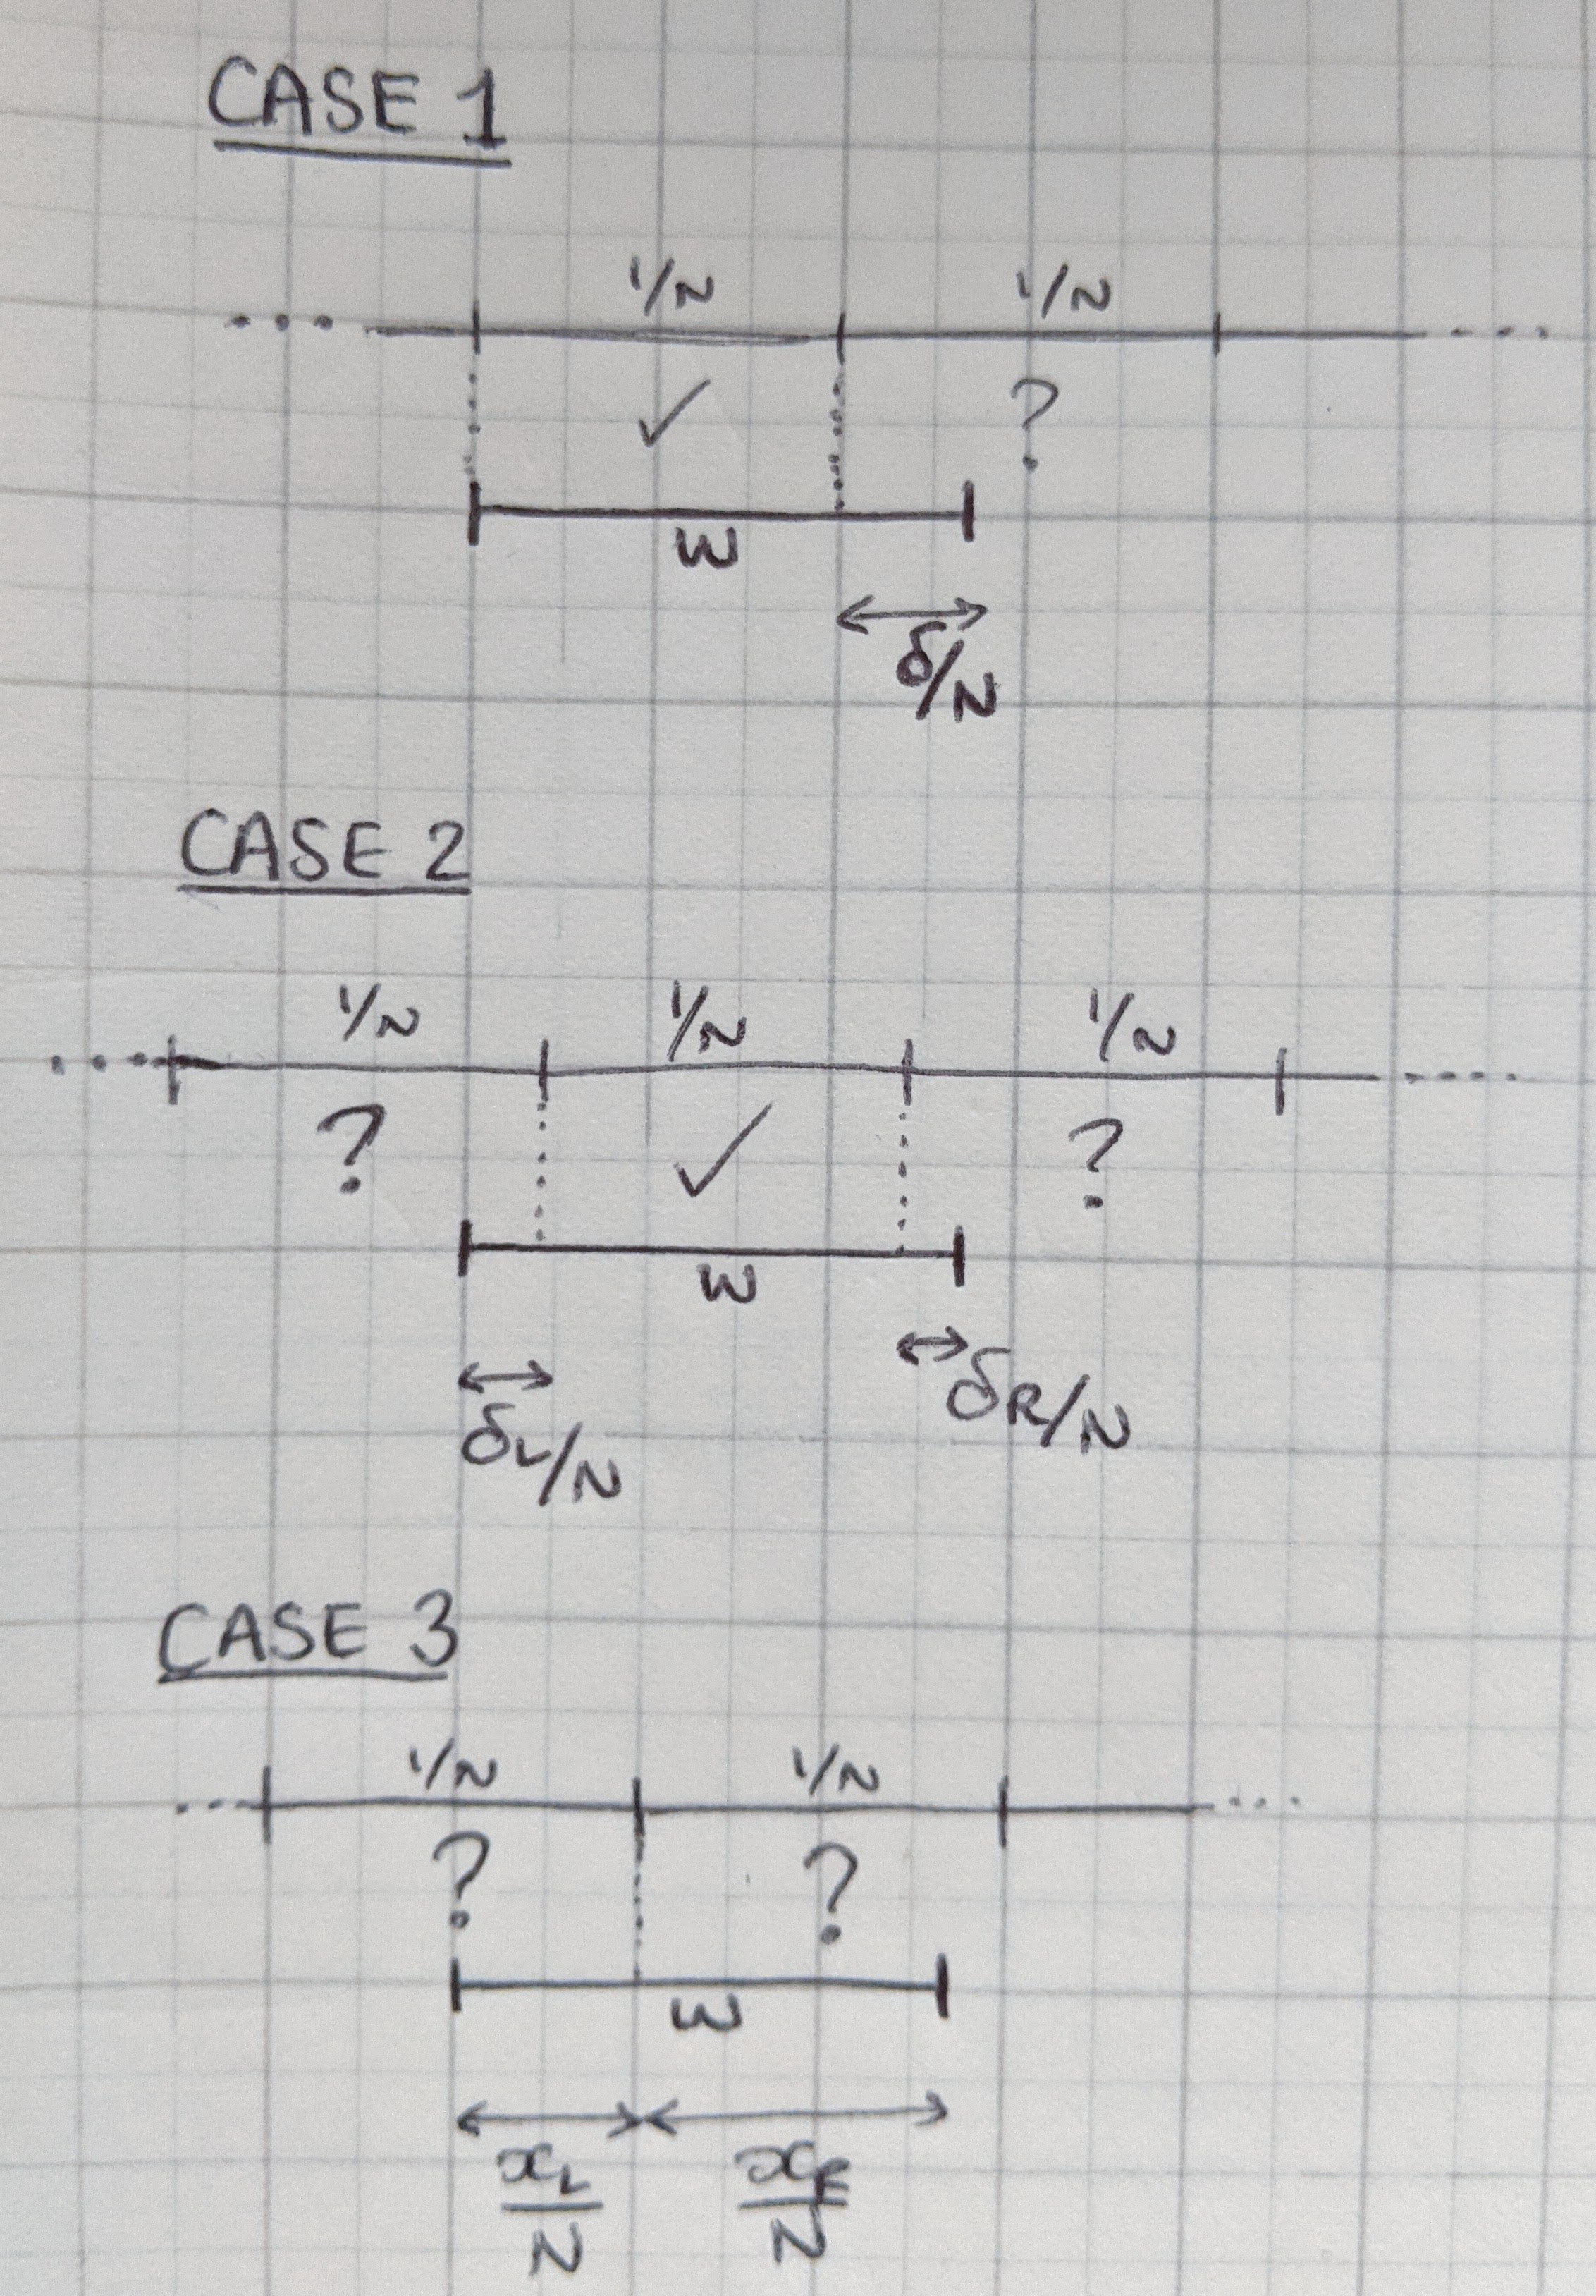
\includegraphics[width=0.4\textwidth]{plots/cases_sketch.jpg}
%\caption[PLACEHOLDER Cases for stratified resampling with a fixed weight]{PLACEHOLDER Cases for stratified resampling with a fixed weight. When I make this properly I need to allow for general $k$ rather than fixing $k=1$ as done here. Case 3 is only valid for $k\geq1$.}
%\label{fig:strat_cases_temp}
%\end{figure}

\begin{figure}
\centering
%\subfloat[Case 1]{
%\begin{tikzpicture}
%% w subinterval
%\draw[thick] (0,0)--(1.9,0);
%\draw[thick,dotted] (1.9,0)--(2.3,0);
%\draw[thick] (2.3,0)--(4.8,0);
%\draw[thick] (0,0.1)--(0,-0.1);
%\draw[thick] (4.8,0.1)--(4.8,-0.1);
%\node[anchor=north] at (2.4,0) {$w$};
%% length labels
%\draw[<->] (0,-0.4)--(4,-0.4);
%\node[anchor=north] at (2,-0.4) {$k/N$};
%\draw[<->] (4,-0.4)--(4.8,-0.4);
%\node[anchor=north] at (4.4,-0.4) {$\delta/N$};
%% sampling interval
%\draw (-0.5,1.5)--(8.5,1.5);
%\draw[dotted] (-1,1.5)--(-0.5,1.5);
%\draw[dotted] (8.5,1.5)--(9,1.5);
%\draw (0,1.6)--(0,1.4);
%\draw (4,1.6)--(4,1.4);
%\draw (8,1.6)--(8,1.4);
%\node[anchor=south] at (2,1.5) {$k/N$};
%\node[anchor=south] at (6,1.5) {$1/N$};
%% vertical dividers
%\draw[dashed, gray] (0,1.4)--(0,0.1);
%\draw[dashed, gray] (4,1.4)--(4,0.1);
%\end{tikzpicture}
%}\\
\subfloat[The overhang is less than $1/N$ and $ \delta_L \in {[0, \delta]} $. The parent under consideration is automatically assigned $K$ offspring, plus up to two more.]{
\begin{tikzpicture}
% w subinterval
\draw[thick] (0,0)--(1.9,0);
\draw[thick,dotted] (1.9,0)--(2.3,0);
\draw[thick] (2.3,0)--(4.8,0);
\draw[thick] (0,0.1)--(0,-0.1);
\draw[thick] (4.8,0.1)--(4.8,-0.1);
\node[anchor=north] at (2.4,0) {$w$};
% length labels
\draw[<->] (0.3,-0.4)--(4.3,-0.4);
\node[anchor=north] at (2,-0.4) {$\frac{K}{N}$};
\draw[<->] (4.3,-0.4)--(4.8,-0.4);
\node[anchor=north] at (4.55,-0.4) {$\frac{\delta-\delta_L}{N}$};
\draw[<->] (0,-0.4)--(0.3,-0.4);
\node[anchor=north] at (0.15,-0.4) {$\frac{\delta_L}{N}$};
% sampling interval
\draw (-4.2,1.5)--(8.8,1.5);
\draw[dotted] (-4.7,1.5)--(-4.2,1.5);
\draw[dotted] (8.8,1.5)--(9.3,1.5);
\draw (-3.7,1.6)--(-3.7,1.4);
\draw (0.3,1.6)--(0.3,1.4);
\draw (4.3,1.6)--(4.3,1.4);
\draw (8.3,1.6)--(8.3,1.4);
\node[anchor=south] at (-1.7,1.5) {$\frac{1}{N}$};
\node[anchor=south] at (2.3,1.5) {$\frac{K}{N}$};
\node[anchor=south] at (6.3,1.5) {$\frac{1}{N}$};
% vertical dividers
\draw[dashed, gray] (0.3,1.4)--(0.3,0.1);
\draw[dashed, gray] (4.3,1.4)--(4.3,0.1);
% fudge bottom space
\draw[white] (0,-1.3)--(1,-1.3);
\end{tikzpicture}
\label{fig:strat_case1}
}\\
\subfloat[The overhang is greater than $1/N$ (this case can only occur when $K\geq1$) and $\delta_L \in (\delta,1)$. The parent under consideration is automatically assigned $K-1$ offspring, plus up to two more.]{
\begin{tikzpicture}
% w subinterval
\draw[thick] (-2,0)--(1.9,0);
\draw[thick,dotted] (1.9,0)--(2.3,0);
\draw[thick] (2.3,0)--(6.8,0);
\draw[thick] (-2,0.1)--(-2,-0.1);
\draw[thick] (6.8,0.1)--(6.8,-0.1);
\node[anchor=north] at (2.4,0) {$w$};
% length labels
\draw[<->] (0.3,-0.4)--(4.3,-0.4);
\node[anchor=north] at (2,-0.4) {$\frac{K-1}{N}$};
\draw[<->] (4.3,-0.4)--(6.8,-0.4);
\node[anchor=north] at (5.55,-0.4) {$\frac{1+\delta-\delta_L}{N}$};
\draw[<->] (-2,-0.4)--(0.3,-0.4);
\node[anchor=north] at (-1.15,-0.4) {$\frac{\delta_L}{N}$};
% sampling interval
\draw (-4.2,1.5)--(8.8,1.5);
\draw[dotted] (-4.7,1.5)--(-4.2,1.5);
\draw[dotted] (8.8,1.5)--(9.3,1.5);
\draw (-3.7,1.6)--(-3.7,1.4);
\draw (0.3,1.6)--(0.3,1.4);
\draw (4.3,1.6)--(4.3,1.4);
\draw (8.3,1.6)--(8.3,1.4);
\node[anchor=south] at (-1.7,1.5) {$\frac{1}{N}$};
\node[anchor=south] at (2.3,1.5) {$\frac{K-1}{N}$};
\node[anchor=south] at (6.3,1.5) {$\frac{1}{N}$};
% vertical dividers
\draw[dashed, gray] (0.3,1.4)--(0.3,0.1);
\draw[dashed, gray] (4.3,1.4)--(4.3,0.1);
% fudge bottom space
\draw[white] (0,-1.3)--(1,-1.3);
\end{tikzpicture}
\label{fig:strat_case2}
}
\caption[Cases for stratified resampling with a fixed weight]{Cases for stratified resampling with a fixed weight $w = (K+\delta)/N$.}
\label{fig:strat_cases}
\end{figure}


In any case $\nu_t^{(i)} \in \{K-1, K, K+1, K+2\}$ almost surely. 
To define a probability distribution over these four values, we introduce the notation
\begin{equation*}
p_j := \Prob[ \nu_t^{(i)} = \flnw +j \mid w_t^{(i)} ] ,
\end{equation*}
for $j=-1,0,1,2$.
%\seb{Change notation to avoid confusion with $p_k^{(i)}$'s in Chapter~\ref{ch:appl}?}
Since the sample within each interval of length $1/N$ is uniform over that interval, we find the probabilities given in Table~\ref{tab:strat_probs}, in terms of $\delta$ and $\delta_L$. The probabilities do not depend on $K$, but of course the corresponding values of $\nu_t^{(i)}$ do.

\begin{table}[ht]
\centering
\begin{tabular}{ c | c c | c c }
\hline\hline
& Case \subref{fig:strat_case1} & Case \subref{fig:strat_case2} & L.B. & U.B. \\
\hline
$p_{-1}$ & 0 & $\delta_L(1+\delta - \delta_L) -\delta$ & 0 & $1/4$ \\
$p_0$ & $1-\delta + \delta_L(\delta -\delta_L)$ 
        & $1+\delta-2\delta_L(1+\delta -\delta_L)$ & $(1-\delta) /2$ 
        & $1 - 3\delta /4$ \\
$p_1$ & $\delta-2\delta_L(\delta -\delta_L)$ & $\delta_L(1+\delta -\delta_L)$ 
        & $\delta /2$ & $(1+\delta)/2$ \\
$p_2$ & $\delta_L(\delta -\delta_L)$ & 0 & 0 & $1/4$ \\
\hline\hline
\end{tabular}
\caption[Distribution of offspring counts under stratified resampling]{Marginal probability distribution of $\nu_t^{(i)}$ conditional on $w_t^{(i)} = (K+\delta)/N$, in terms of $\delta$ and the left overhang $\delta_L$, along with upper and lower bounds on these in terms of $\delta$ only, which hold in both cases.}
\label{tab:strat_probs}
\end{table}

%By considering the constraints on $\delta_L, \delta_R, x_L, x_R$, we also have the following properties which hold in every case (i.e.\ for any $w_t^{(i)}$):
%\begin{itemize}
%\item $p_{-1} \leq 1/4$
%\item $p_{2} \leq 1/4$
%\item only one of $p_{-1}, p_2$ can be non-zero.
%\end{itemize}





\subsubsection{Systematic resampling}
%\label{sec:resampling_systematic}
Systematic resampling is described in \textcite{carpenter1999} and also in \textcite{whitley1994} where it is called ``stochastic universal sampling''.

Like stratified resampling, it uses the inversion sampler of multinomial resampling but starts with a more regular set of points in $[0,1]$.
In this scheme, only one standard Uniform sample is drawn, $u \sim \Unif[0,1]$, from which the $N$ samples are generated by via the transformation
\begin{equation*}
U_i = \frac{u+ i-1}{N}
\end{equation*}
for $i = 1, \dots, N $.
The parental indices are again selected according to \eqref{eq:syst_strat_resampling}, as illustrated in Figure \ref{fig:inv_resampling}.

\textcite{kitagawa1996} suggests a deterministic scheme in which the random $u$ is replaced by a fixed $\alpha\in[0,1]$; but, being deterministic, this scheme does not satisfy the unbiasedness condition (Property~\ref{item:resampling_property1} in Definition~\ref{defn:resampling}).
\textcite{whitley1994} employs a different description of systematic resampling, where the interval $[0,1]$ is joined up into a circle, and the systematic samples are evenly spaced pointers on an outer ring, which is spun around like a roulette wheel (Figure~\ref{fig:roulettewheel}). This comprises adding a random phase to each $U_i$, modulo one, and is an exactly equivalent description of systematic resampling.

\begin{figure}[ht]
\centering
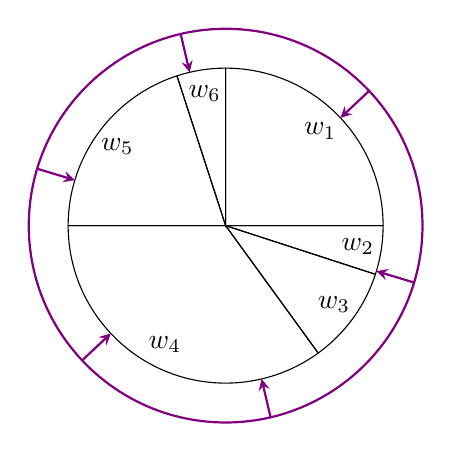
\begin{tikzpicture}[>=stealth]
\draw (0,0)--(0:2) arc(0:90:2)--cycle;
\node at (45:1.7) {$w_1$};
\draw (0,0)--(342:2) arc(342:360:2)--cycle;
\node at (351:1.7) {$w_2$};
\draw (0,0)--(306:2) arc(306:342:2)--cycle;
\node at (324:1.7) {$w_3$};
\draw (0,0)--(180:2) arc(180:306:2)--cycle;
\node at (243:1.7) {$w_4$};
\draw (0,0)--(108:2) arc(108:180:2)--cycle;
\node at (144:1.7) {$w_5$};
\draw (0,0)--(90:2) arc(90:108:2)--cycle;
\node at (99:1.7) {$w_6$};
%% outer circle
\draw[thick, violet] (0,0) circle (2.5);
%% arrows spaced 1/N
\draw[->, thick, violet] (43.2:2.5)--(43.2:2);
\draw[->, thick, violet] (103.2:2.5)--(103.2:2);
\draw[->, thick, violet] (163.2:2.5)--(163.2:2);
\draw[->, thick, violet] (223.2:2.5)--(223.2:2);
\draw[->, thick, violet] (283.2:2.5)--(283.2:2);
\draw[->, thick, violet] (343.2:2.5)--(343.2:2);
\end{tikzpicture}
\caption[Whitley's roulette wheel]{Whitley's ``roulette wheel'' description of systematic resampling. The inner circle stays fixed while the outer circle with its equally-spaced pointers is ``spun'' by a random amount. The weights and phase pictured are the same as in Figure~\ref{fig:inv_resampling}, with $N=6$. For systematic resampling, the two descriptions are equivalent.}
\label{fig:roulettewheel}
\end{figure}

Like stratified resampling, systematic resampling ensures the random numbers are ``well spread out''; the resulting samples are even more constrained than with stratified resampling. 
Systematic resampling also has the advantage of being extremely easy to implement and computationally efficient, requiring only one sample from a pseudo-random number generator (PRNG) followed by $O(N)$ elementary operations.

However, the systematic scheme is known to exhibit pathological behaviour in some cases because its performance depends on the ordering of the weights. A simple example of this phenomenon is presented in \textcite{douc2005}. 
Such behaviour can be avoided by randomly permuting the weights before resampling, and this is the recommended practice. 



\subsubsection{Star resampling}
%\label{sec:resampling_star}
For the sake of comparison, we also construct a resampling scheme which is in some sense the worst possible.
Sample
\begin{equation*}
a \sim \Cat( \{1,\dots, N\}, w_t^{(1:N)} )
\end{equation*}
and set $a_t^{(i)} = a$ for all $i$.
The resulting offspring counts are all equal to zero except for $\nu_t^{(a)}$, which is equal to $N$.
This resampling scheme is indeed unbiased, since each offspring count has marginal distribution
\begin{equation*}
\nu_t^{(i)}  \mid w_t^{(1:N)} 
= \begin{cases}
0 & \text{w.p. } 1-w_t^{(i)} \\
N & \text{w.p. } w_t^{(i)} .
\end{cases}
\end{equation*}
These offspring counts have the highest possible marginal variance subject to $\E[ \nu_t^{(i)}  \mid w_t^{(i)} ] = Nw_t^{(i)}$ and $\nu_t^{(i)} \in \{0,\dots,N\}$.

I call this scheme \emph{star resampling} because the parent-offspring relationships at each iteration form a star graph.


\subsubsection{Minimal variance branching}
The minimal variance branching (MVB) algorithm of \textcite{crisan1999} provides a framework for resampling that enforces the minimal variance. 
It requires that each offspring count $\nu_t^{(i)}$, conditionally on $w_t^{(i)}$, has marginal distribution
\begin{equation}\label{eq:branching_distn}
\nu_t^{(i)} \mid w_t^{(i)} \eqdist \flnw + \Bern(Nw_t^{(i)} - \flnw) .
\end{equation}
We will see later on that this is exactly the framework of \emph{stochastic rounding}.

The set-up of \textcite{crisan1999} does not require the number of particles to remain constant from one generation to the next (Property~\ref{item:resampling_property1} in Definition~\ref{defn:resampling}), so the MVB algorithm could be implemented for instance by sampling each $\nu_t^{(i)}$ independently from \eqref{eq:branching_distn}. The authors remark that enforcing strictly negative correlation between the offspring counts can improve the rate of convergence, but they do not specify how this might be achieved.
Since we are not given a specific implementation, MVB is not discussed much in the remainder of the chapter, and is for instance omitted from Table~\ref{tab:resampling_properties} since many of the properties included there are not well-defined for MVB.



\subsubsection{Srinivasan sampling procedure}
\textcite{gerber2017} build on the work of \textcite{crisan1999} in that they construct a resampling scheme for which the marginal offspring counts are distributed as \eqref{eq:branching_distn}, but the number of particles is held constant and non-negative correlation of offspring counts is enforced. The resulting scheme is termed \emph{Srinivasan sampling procedure (SSP) resampling} after \textcite{srinivasan2001}.

The implementation is somewhat complicated compared to the other schemes we have seen \parencite[for full details see][Algorithm~1]{gerber2017} but a brief description is given here.
The offspring counts are initialised at $Nw_t^{(i)}$, then we iterate through pairs of counts, rounding one of the pair up and the other down by an amount such that at least one of the pair ends up an integer. After at most $N$ such adjustments, all of the counts are integers and can be returned. Each iteration adds and subtracts the same amount so that the sum of the counts is preserved, ensuring that the number of particles remains constant. Which of the selected pair is increased/decreased in each iteration is chosen at random with probabilities that guarantee the resampling is unbiased.

As well as proposing this resampling scheme, \textcite{gerber2017} make several other contributions to the SMC resampling literature, some of which will be discussed later.


\begin{table}[ht]
\centering
\begin{tabular}{ l l }
\hline\hline
Abbreviation & Description \\% & Defined in Section \\
\hline
\texttt{multi} & multinomial resampling \\%& \ref{sec:resampling_multinomial} \\
\texttt{star} & star resampling \\%& \ref{sec:resampling_star} \\
\texttt{strat} & stratified resampling \\%& \ref{sec:resampling_stratified} \\
\texttt{syst} & systematic resampling \\%& \ref{sec:resampling_systematic} \\
\texttt{res-multi} & residual resampling with multinomial residuals \\
        %& \ref{sec:resampling_residual} \\
\texttt{res-star} & residual resampling with star residuals \\
        %& \ref{sec:resampling_residual} \\
\texttt{res-strat} & residual resampling with stratified residuals \\
        %& \ref{sec:resampling_residual} \\
\texttt{res-syst} & residual resampling with systematic residuals \\
        %& \ref{sec:resampling_residual} \\
\texttt{ssp} & Srinivasan sampling procedure resampling \\%& \\
%\texttt{mvb} & minimal variance branching algorithm \\%& \\
\hline\hline
\end{tabular}
\caption{Abbreviations for resampling schemes}
\label{tab:resampling_abbrevs}
\end{table} 





\subsection{Properties}\label{sec:resampling_properties}
In this section we consider some important properties of resampling schemes, and see how the example schemes of Section~\ref{sec:examples_resamplingschemes} compare in terms of these.
The findings are summarised in Table~\ref{tab:resampling_properties}, with the exception of a few properties which depend on details of the implementation or are applicable only to a subset of the resampling schemes considered.


\subsubsection{Support of offspring numbers}
Recall that the weights give an indication of how ``useful'' each particle is for the approximation. Killing a high-weight particle is likely to increase the variance of the SMC estimates, while duplicating a low-weight particle wastes computational resources on propagating particles that will not contribute much to reducing that variance.
One way to assess the performance of a given resampling scheme, then, is to consider the support of the marginal offspring distributions, conditional on the weights. This tells us how many duplicates it is possible to obtain from a particle with a given weight, and is therefore an indication of performance, albeit a rather crude one.

Suppose that $w_t^{(i)} \in [K/N, (K+1)/N]$. The value of $K$ roughly determines how useful particle $i$ is. Conditional on $K$, we will determine the range of possible values $\nu_t^{(i)}$ can take, under each  of the resampling schemes described in Section~\ref{sec:examples_resamplingschemes}.

Under multinomial resampling, it is possible for $\nu_t^{(i)}$ to take any value from $0$ to $N$ (although some values are of course more likely than others).
Thus it is possible for a high-weight particle to have zero offspring, or a low-weight particle to have many offspring, simply by chance.

Residual resampling ensures that every particle with above-average (i.e.\ $>1/N$) weight has at least one offspring, avoiding the loss of high-weight particles. If the residuals are sampled using multinomial resampling then the duplication of low-weight particles is not avoided, $\nu_t^{(i)} \in \{K, \dots, K+R\} \subseteq \{K,\dots, N\}$, but this can be addressed by using a lower-variance scheme for the residual offspring. Various choices are included in Table~\ref{tab:resampling_properties}.

Stratified resampling is more restrictive, $\nu_t^{(i)} \in \{ K-1, K, K+1, K+2 \}$, but allows the possibility of a particle with above-average weight having no offspring. This is not quite as good as the erroneous claim of \textcite{douc2005} that $| \nu_t^{(i)} - Nw_t^{(i)} | \leq 1$ for stratified resampling.
Systematic resampling has the smallest support, $\nu_t^{(i)} \in \{K, K+1\}$, that is possible whilst maintaining unbiasedness, as do SSP and MVB resampling.

Another way to quantify this property is by considering the maximum possible difference between the offspring count $\nu_t^{(i)}$ and its expected value $N w_t^{(i)}$. This is also presented in Table~\ref{tab:resampling_properties}.




\subsubsection{Degeneracy under equal weights}
In the case where all of the weights are multiples of $1/N$, low-variance schemes such as residual and systematic resampling become fully deterministic. 
Since $\flnw = Nw_t^{(i)}$ for each $i$, residual resampling will have $R=0$, leaving no remainder to be assigned stochastically. 
In systematic resampling exactly $\flnw = Nw_t^{(i)}$ samples will fall in the $i^{th}$ interval.
In particular, if $w_t^{(1:N)} = (1,\dots, 1)/N$ then each parent is assigned exactly one offspring deterministcially, so there is effectively no resampling.

The same phenomenon occurs with stratified resampling, although not if one uses Whitley's roulette wheel description (Figure~\ref{fig:roulettewheel}). The random phase shift introduced by ``spinning the wheel'' prevents the inversion sampling intervals from lining up exactly with the weight intervals, so the resampled offspring counts may vary from their means by one either side.
\textcite{whitley1994} does not describe stratified resampling, but we see that unlike with systematic resampling, in the case of startified resampling the roulette wheel description is not equivalent to the standard inversion sampling description. 
The roulette wheel adds some unnecessary extra randomness, so the straightforward inversion sampler is preferred.

When the state space is continuous, it is often the case that the event that all weights are multiples of $1/N$ has zero measure. Even so, with non-zero probability we may get arbitrarily close to this regime in which resampling becomes deterministic.




\subsubsection{Marginal variance of offspring counts}
%\draft{Mention negative association? $=$ teaser for later, which has to do with covariance between counts rather than marginal variance.}
Another indication of the performance of resampling is the variance of the resampled offspring counts. For instance we might ask what is the marginal variance of $\nu_t^{(i)}$, conditional on the corresponding weight $w_t^{(i)}$. We would like to keep this variance small, limiting the additional randomness introduced to our Monte Carlo estimates by the resampling step.

In multinomial resampling, the marginal distributions are
\begin{equation*}
\nu_t^{(i)} \mid w_t^{(i)} 
\eqdist \Bin(N, w_t^{(i)})
\end{equation*}
so the variance is
\begin{equation*}
\V[ \nu_t^{(i)} \mid w_t^{(i)} ]
= N w_t^{(i)} ( 1- w_t^{(i)} ) .
\end{equation*}
Compare this to star resampling, where the marginal offspring counts
\begin{equation*}
\nu_t^{(i)} \mid w_t^{(i)} 
\eqdist N \Bern( w_t^{(i)} )
\end{equation*}
having variance
\begin{equation*}
\V[ \nu_t^{(i)} \mid w_t^{(i)} ]
= N^2 w_t^{(i)} ( 1- w_t^{(i)} ) ,
\end{equation*}
$N$ times larger than in the multinomial case.

As pointed out in \textcite[p.557]{crisan1999}, their MVB process yields offspring variance
\begin{equation*}
\V[ \nu_t^{(i)} \mid w_t^{(i)} ]
= ( Nw_t^{(i)} -\flnw )(1- Nw_t^{(i)} + \flnw) 
\leq \frac{1}{4} ,
\end{equation*}
since the stochastic part of $\nu_t^{(i)}$ is a $\Bern( Nw_t^{(i)} -\flnw )$ random variable (as seen in \eqref{eq:branching_distn}).
The same marginal variance appears from systematic, residual-systematic and SSP resampling, since these all share the same marginal offspring distributions. We will see in Section~\ref{sec:SRs} that all of these schemes fall within the \emph{stochastic rounding} class, and marginal offspring variance is a property shared by all stochastic roundings.

The marginal variance is harder to calculate for other schemes such as residual-multi\-nomial and stratified resampling because these were not defined in terms of marginal distributions, nor are the offspring counts independent conditional on the weights.
However, it is possible in some cases to find upper bounds on the variance, and some such bounds are derived below.

In residual-multinomial resampling, $\nu_t^{(i)}$ depends on all of the other weights as well as $w_t^{(i)}$, but only through the statistic $R := \sum (N w_t^{(i)} - \flnw)$.
We have
\begin{equation*}
\nu_t^{(i)} \mid w_t^{(i)} , R
\eqdist \flnw + \Bin\left( R, \frac{Nw_t^{(i)} - \flnw}{R} \right) .
\end{equation*}
Using the law of total variance,
\begin{align*}
\V[ \nu_t^{(i)} \mid w_t^{(i)} ]
&= \E\left[ \V[ \nu_t^{(i)} \mid w_t^{(i)}, R ] \mid w_t^{(i)} \right]
        + \V\left[ \E[ \nu_t^{(i)} \mid w_t^{(i)}, R ] \mid w_t^{(i)} \right] \\
&= \E\left[ (Nw_t^{(i)} - \flnw) \left( 1- \frac{Nw_t^{(i)} - \flnw}{R} \right) 
        \mid w_t^{(i)} \right] \\
    &\qquad+ \V\left[ Nw_t^{(i)} \mid w_t^{(i)} \right] \\
&= Nw_t^{(i)} - \flnw - (Nw_t^{(i)} - \flnw)^2\, \E[ R^{-1} \mid w_t^{(i)} ] \\
% &\leq \E\left[ Nw_t^{(i)} - \flnw \mid w_t^{(i)} \right]
%        + \V\left[ Nw_t^{(i)} \mid w_t^{(i)} \right] \\
&\leq Nw_t^{(i)} - \flnw .
\end{align*}
Here we have excluded the case $R=0$, in which the variance is zero.
Similarly, for residual resampling with star residuals,
\begin{equation*}
\nu_t^{(i)} \mid w_t^{(i)} , R
\eqdist \flnw + R \Bern\left( \frac{Nw_t^{(i)} - \flnw}{R} \right) .
\end{equation*}
and we find
\begin{align*}
\V[ \nu_t^{(i)} \mid w_t^{(i)} ]
&= \E\left[ \V[ \nu_t^{(i)} \mid w_t^{(i)}, R ] \mid w_t^{(i)} \right]
        + \V\left[ \E[ \nu_t^{(i)} \mid w_t^{(i)}, R ] \mid w_t^{(i)} \right] \\
&= \E\left[ R (Nw_t^{(i)} - \flnw) \left( 1- \frac{Nw_t^{(i)} - \flnw}{R} \right) 
        \mid w_t^{(i)} \right] \\
    &\qquad+ \V\left[ Nw_t^{(i)} \mid w_t^{(i)} \right] \\
&= \E\left[ R (Nw_t^{(i)} - \flnw) \left( 1- \frac{Nw_t^{(i)} - \flnw}{R} \right) 
        \mid w_t^{(i)} \right] \\
&= (Nw_t^{(i)} - \flnw) \E\left[ R \mid w_t^{(i)} \right]  - (Nw_t^{(i)} - \flnw)^2 \\
&\leq N (Nw_t^{(i)} - \flnw) .
\end{align*}
Again, if $R=0$ then the variance is zero.

For stratified resampling, we can use the constraints on the marginal offspring distribution that were derived in Section~\ref{sec:examples_resamplingschemes}. Recall that, conditional on $w_t^{(i)}$, $\nu_t^{(i)} = \flnw + j$ with probability $p_{j}$ for $j=-1,0,1,2$.
We can use the expressions for $p_{-1},p_0,p_1,p_2$ in the two cases of Figure~\ref{fig:strat_cases}, as summarised in Table~\ref{tab:strat_probs}, to bound the variance. First write
\begin{align}
\V\left[ \nu_t^{(i)} \mid w_t^{(i)} \right]
&= \V\left[ \nu_t^{(i)} - \flnw \mid w_t^{(i)} \right] \notag\\
&= \E\left[ (\nu_t^{(i)} - \flnw)^2 \mid w_t^{(i)} \right] 
        - \E\left[ \nu_t^{(i)} -\flnw \mid w_t^{(i)} \right]^2 \notag\\
&= p_{-1} + p_1 + 4p_2 - (-p_{-1} + p_1 + 2p_2)^2 . \label{eq:marg_var_strat}
%\leq 1/2 .
\end{align}
%In Case~\subref{fig:strat_case1}, 
Using the upper and lower bounds in Table~\ref{tab:strat_probs} and then optimising over $\delta$, we obtain the bound
\begin{equation*}
\V[ \nu_t^{(i)} \mid w_t^{(i)} ]
\leq \frac{1}{4} + \frac{1+\delta}{2} + 1 - ( 0 + \frac{\delta}{2} + 0 )^2
=\frac{1}{4}(7 + 2\delta - \delta^2)
\leq 2 .
%= (\delta -2\delta_L\delta_R + 4\delta_L\delta_R) 
%        - (\delta - 2\delta_L\delta_R + 2\delta_L\delta_R)^2
%= \delta +2\delta_L\delta_R - \delta^2
\end{equation*}
Optimising the exact expressions in each case (first two columns in Table~\ref{tab:strat_probs}) does not improve this overall bound.
%which is maximised at $\delta_L=\delta_R=\delta/2$ for a maximum variance of $\delta(1-\delta/2)$, which is at most $1/2$.
%In Case~\subref{fig:strat_case2}, we have
%\begin{equation*}
%\V[ \nu_t^{(i)} \mid w_t^{(i)} ]
%= (x_Lx_R -\delta + x_Lx_R) - (-x_Lx_R + \delta + x_Lx_R)^2
%= \delta + 2x_Lx_R -\delta^2
%\end{equation*}
%which is maximised at $x_L=x_R=(1+\delta)/2$ for a maximum variance of $(1-\delta^2)/2$\seb{wrong!}, which is at most $1/2$.
%Overall we have the bound
%\begin{equation*}
%\V[ \nu_t^{(i)} \mid w_t^{(i)} ]
%\leq \frac{1}{2}
%\end{equation*}
%for any $w_t^{(1:N)}$.

Residual-stratified resampling has the further constraint that $p_{-1} =0$ (i.e.\ Figure~\ref{fig:strat_case2} doesn't occur) since the residual weights are between $0$ and $1/R$. Now the bounds in Table~\ref{tab:strat_probs} are too loose, so we bound the variance by using the exact expressions from Table~\ref{tab:strat_probs} in each case and optimising over $\delta_L, \delta$.
Setting $p_{-1}=0$ in \eqref{eq:marg_var_strat}, substituting the expressions for Case~\subref{fig:strat_case1} from Table~\ref{tab:strat_probs}, and maximising over $\delta_L$ and then $\delta$ yields
\begin{align*}
\V[ \nu_t^{(i)} \mid w_t^{(i)} ]
&= p_1 + 4p_2 - (p_1 + 2p_2)^2 
= \delta - 2\delta_L(\delta-\delta_L) + 4\delta_L(\delta-\delta_L) -\delta^2 \\
&= \delta - \delta^2 + 2\delta\delta_L - 2\delta_L^2
\leq \delta - \frac{1}{2}\delta^2
\leq \frac{1}{2} ,
\end{align*}
since the maximum is achieved at $\delta_L = \delta/2$ and then at $\delta=1$.
%% THERE IS NO CASE B FOR RES-STRAT!
%Similarly, for Case~\subref{fig:strat_case2},
%\begin{equation*}
%\V[ \nu_t^{(i)} \mid w_t^{(i)} ]
%= p_1 + 4p_2 - (p_1 + 2p_2)^2 
%= \delta_L(1+\delta-\delta_L) - (\delta_L(1+\delta-\delta_L))^2
%\leq \frac{1}{4} .
%\end{equation*}
%Combining the two cases, we obtain an overall variance bound
%\begin{equation*}
%\V[ \nu_t^{(i)} \mid w_t^{(i)} ]
%\leq \frac{1}{2}
%\end{equation*}
%for residual-stratified resampling.

Table~\ref{tab:resampling_properties} includes upper bounds on $\V[\nu_t^{(i)}]$ for various resampling schemes, independent of $w_t^{(i)}$. Those general bounds are derived from the results of this section, bounded above independently of the weights. Some of the bounds may not be tight.
We could also try to bound this variance below, but for every resampling scheme the only lower bound valid for all $w_t^{(i)}$ is zero (consider the case $w_t^{(i)}=0$) so this does not provide any more information.





\subsubsection{Contribution to the Monte Carlo variance}
While the variance of the offspring counts goes some way towards providing a comparison between resampling schemes, a more relevant property is the contribution of the resampling step to the Monte Carlo variance.
This quantifies directly the effect of a certain choice of resampling scheme on the variance of the resulting Monte Carlo estimators.

Let $(\mathcal{G}_t)_{t\geq0}$ be the filtration generated by the particle positions and weights up to and including time $t$, so $\mathcal{G}_t$ is the $\sigma$-algebra generated by $( X_{0:t}^{(1:N)} , w_{0:t}^{(1:N)} )$.
Consider the position of the $i$th particle in generation $t+1$ just after resampling but before mutating, that is $X_t^{(a_t^{(i)})}$.
Define the one-step Monte Carlo variance induced by resampling as
\begin{equation}\label{eq:resamplingMCvariance}
\sigma(\varphi) 
:= \V\left[ \frac{1}{N} \sum_{i=1}^N \varphi ( X_t^{(a_t^{(i)})} ) \midd \mathcal{G}_t \right]
\end{equation}
where $\varphi$ is an arbitrary test function.

Some results comparing this variance across different resampling schemes are presented in \textcite{douc2005}. 
Their results, plus some additional ones, are presented in Proposition~\ref{thm:resampling_var_compare}.
It may be possible to derive similar results regarding residual-stratified and SSP resampling, but such results are hard to obtain due to the strong dependence between parental indices induced by these resampling schemes. 
This remains an interesting open problem.

In the case of systematic (but not necessarily residual-systematic) resampling, no such variance comparison can be made. Systematic resampling generally yields low variance in practice, but it is possible to construct pathological cases in which it yields higher variance than multinomial resampling \parencite[Section 3.4]{douc2005} and it lacks theoretical support more generally \parencite[e.g.][Section 3.3]{gerber2017}.

\begin{prop}[Variance of resampling schemes]\label{thm:resampling_var_compare}
Let $\sigma_{\texttt{multi}}$ etc.\ denote the variance \eqref{eq:resamplingMCvariance} under the various resampling schemes, as abbreviated in Table~\ref{tab:resampling_abbrevs}.
For any square-integrable function $\varphi$,
\begin{enumerate}[label=(\alph*)]
\item \label{item:resampling_var1} \hspace{5pt}
$\begin{aligned}
    \sigma_{\texttt{multi}}(\varphi) 
    \geq \sigma_{\texttt{res-multi}}(\varphi)
\end{aligned}$
\item \label{item:resampling_var2} \hspace{5pt}
$\begin{aligned}
    \sigma_{\texttt{multi}}(\varphi) 
    \geq \sigma_{\texttt{strat}}(\varphi)
\end{aligned}$
\item \label{item:resampling_var3} \hspace{5pt}
$\begin{aligned}
    \sigma_{\texttt{star}}(\varphi) 
    = N \sigma_{\texttt{multi}}(\varphi)
\end{aligned}$
\item \label{item:resampling_var4} \hspace{5pt}
$\begin{aligned}
    \sigma_{\texttt{res-star}}(\varphi) 
    \geq \sigma_{\texttt{res-multi}}(\varphi) 
    \geq \sigma_{\texttt{res-strat}}(\varphi)
\end{aligned}$
\item \label{item:resampling_var5} \hspace{5pt}
$\begin{aligned}
    \sigma_{\texttt{star}}(\varphi) 
    \geq \sigma_{\texttt{res-star}}(\varphi) 
\end{aligned}$
\end{enumerate}
\end{prop}
The partial ordering suggested by Proposition~\ref{thm:resampling_var_compare} is depicted graphically in Figure~\ref{fig:condvar_ordering}.

\begin{figure}[ht]
\centering
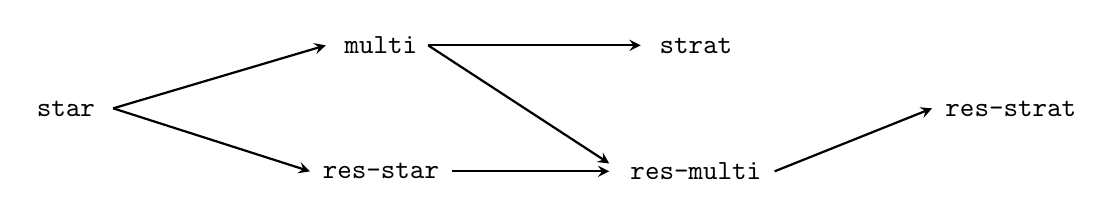
\begin{tikzpicture}[>=stealth]
\node at (0,0) {\texttt{star}};
\node at (4,0.8) {\texttt{multi}};
\node at (4,-0.8) {\texttt{res-star}};
\node at (8,0.8) {\texttt{strat}};
\node at (8,-0.8) {\texttt{res-multi}};
\node at (12,0) {\texttt{res-strat}};
\draw[->, thick] (0.6,0)--(3.3,0.8); %% star -> multi
\draw[->, thick] (0.6,0)--(3.1,-0.8); %% star -> res-star
\draw[->, thick] (4.6,0.8)--(7.3,0.8); %% multi -> strat
\draw[->, thick] (4.9,-0.8)--(6.9,-0.8); %% res-star -> res-multi
\draw[->, thick] (4.6,0.8)--(6.9,-0.7); %% multi -> res-multi
\draw[->, thick] (9,-0.8)--(11,0); %% res-multi -> res-strat
\end{tikzpicture}
\caption[Conditional variance inequalities between resampling schemes]{Graphical depiction of the conditional variance inequalities stated in Proposition~\ref{thm:resampling_var_compare}.
Conditional variance \eqref{eq:resamplingMCvariance} is non-increasing along arrows.}
\label{fig:condvar_ordering}
\end{figure}

\begin{proof}
\textbf{\ref{item:resampling_var1}} See \textcite[Section 3]{douc2005}.\\
\textbf{\ref{item:resampling_var2}} See \textcite[Section 3]{douc2005}.\\
\textbf{\ref{item:resampling_var3}}
The following expression is derived in \textcite[Equation (6)]{douc2005}:
\begin{equation*}
\sigma_{\texttt{multi}}(\varphi)
= \frac{1}{N} \sum_{j=1}^N \varphi^2(X_t^{(j)}) w_t^{(j)}
        - \frac{1}{N} \left\{ \sum_{j=1}^N \varphi(X_t^{(j)}) w_t^{(j)} \right\}^2 .
\end{equation*}
Under star resampling, all of the resampled indices are equal, say $X_t^{(a_t^{(1)})} = \dots = X_t^{(a_t^{(N)})} = X_t^\star$, so
\begin{align}
\sigma_{\texttt{star}}(\varphi)
&= \V\left[ \frac{1}{N} \sum_{i=1}^N \varphi( X_t^{(a_t^{(i)})} ) \midd \mathcal{G}_t \right]
= \V\left[ \varphi( X_t^\star) \mid \mathcal{G}_t \right] \notag\\
&= \E\left[ \varphi^2( X_t^\star) \mid \mathcal{G}_t \right]
        - \E\left[ \varphi( X_t^\star) \mid \mathcal{G}_t \right]^2 \notag\\
&= \sum_{j=1}^N \varphi^2(X_t^{(j)}) 
        \Prob[ X_t^\star = X_t^{(j)} \mid \mathcal{G}_t ]
        - \left\{ \sum_{j=1}^N \varphi(X_t^{(j)}) 
        \Prob[ X_t^\star = X_t^{(j)} \mid \mathcal{G}_t ] \right\}^2 \notag\\
&= \sum_{j=1}^N \varphi^2(X_t^{(j)}) w_t^{(j)}
        - \left\{ \sum_{j=1}^N \varphi(X_t^{(j)}) w_t^{(j)} \right\}^2 \label{eq:condvar_star}\\
&= N \sigma_{\texttt{multi}}(\varphi) , \notag
\end{align}
as required.\\
\textbf{\ref{item:resampling_var4}} The second inequality follows from \ref{item:resampling_var2} and is stated in \textcite[p.9]{gerber2017}.
For the first inequality, we use the following expression which is a slight modification of \textcite[Equation (8)]{douc2005}:
\begin{equation*}
\sigma_{\texttt{res-multi}}(\varphi)
= \frac{R}{N^2} \sum_{j=1}^N \varphi^2(X_t^{(j)}) r^{(j)}
        - \frac{R}{N^2} \left( \sum_{j=1}^N \varphi(X_t^{(j)}) r^{(j)} \right)^2 .
\end{equation*}
A derivation similar to theirs can also be used for residual-star resampling. 
First notice that, conditional on $\mathcal{G}_t$, the Monte Carlo estimate in \eqref{eq:resamplingMCvariance} can be decomposed into a sum of conditionally deterministic terms plus a sum of stochastic terms:
\begin{equation*}
\frac{1}{N} \sum_{i=1}^N \varphi( X_t^{(a_t^{(i)})} )
= \frac{1}{N} \sum_{j=1}^N \flnw[j] \varphi (X_t^{(j)})
        + \frac{1}{N} \sum_{i=1}^R \varphi (\hat{X}_t^{(i)}) ,
\end{equation*}
where the terms in the second sum are all equal, say $\hat{X}_t^{(1)} = \dots = \hat{X}_t^{(R)} = X_t^\star$.
The first sum is conditionally deterministic and hence does not contribute to the Monte Carlo variance \eqref{eq:resamplingMCvariance}.
We have
\begin{align}
\sigma_{\texttt{res-star}}(\varphi)
&= \V\left[ \frac{1}{N} \sum_{i=1}^R \varphi (\hat{X}_t^{(i)}) \midd \mathcal{G}_t \right] 
= \frac{R^2}{N^2} \V\left[ \varphi (X_t^\star) \midd \mathcal{G}_t \right] \notag\\
&= \frac{R^2}{N^2} \E\left[ \varphi^2( X_t^\star) \mid \mathcal{G}_t \right]
        - \frac{R^2}{N^2} \E\left[ \varphi( X_t^\star) \mid \mathcal{G}_t \right]^2 \notag\\
&= \frac{R^2}{N^2} \sum_{j=1}^N \varphi^2(X_t^{(j)}) 
        \Prob[ X_t^\star = X_t^{(j)} \mid \mathcal{G}_t ]
        - \frac{R^2}{N^2} \left\{ \sum_{j=1}^N \varphi(X_t^{(j)}) 
        \Prob[ X_t^\star = X_t^{(j)} \mid \mathcal{G}_t ] \right\}^2 \notag\\
&= \frac{R^2}{N^2} \sum_{j=1}^N \varphi^2(X_t^{(j)}) r^{(j)}
        - \frac{R^2}{N^2} \left\{ \sum_{j=1}^N \varphi(X_t^{(j)}) r^{(j)} \right\}^2 \label{eq:condvar_resstar}\\
&= R \sigma_{\texttt{res-multi}}(\varphi) \notag\\
&\geq \sigma_{\texttt{res-multi}}(\varphi) \notag
\end{align}
whenever $R\geq 1$. 
If $R=0$ then all residual schemes have zero variance and \ref{item:resampling_var4} holds trivially.\\
\textbf{\ref{item:resampling_var5}}
We have from \eqref{eq:condvar_star}
\begin{equation*}
\sigma_{\texttt{star}}(\varphi)
= \sum_{j=1}^N \varphi^2(X_t^{(j)}) w_t^{(j)}
        - \left\{ \sum_{j=1}^N \varphi(X_t^{(j)}) w_t^{(j)} \right\}^2
\end{equation*}
and from \eqref{eq:condvar_resstar}, noting that $r^{(j)} := (Nw_t^{(j)} - \flnw[j])/R \leq Nw_t^{(j)}/R$,
\begin{align*}
\sigma_{\texttt{res-star}}(\varphi)
&= \frac{R^2}{N^2} \sum_{j=1}^N \varphi^2(X_t^{(j)}) r^{(j)}
        - \frac{R^2}{N^2} \left\{ \sum_{j=1}^N \varphi(X_t^{(j)}) r^{(j)} \right\}^2 \\
&\leq \frac{R^2}{N^2} \sum_{j=1}^N \varphi^2(X_t^{(j)}) \frac{ N w_t^{(j)} }{R}
        - \frac{R^2}{N^2} \left\{ \sum_{j=1}^N \varphi(X_t^{(j)}) \frac{ N w_t^{(j)} }{R} \right\}^2 \\
&= \frac{R}{N} \sum_{j=1}^N \varphi^2(X_t^{(j)}) w_t^{(j)}
        - \left\{ \sum_{j=1}^N \varphi(X_t^{(j)}) w_t^{(j)} \right\}^2 \\
&\leq \sigma_{\texttt{star}}(\varphi) ,
\end{align*}
since $R\leq N-1$.
\end{proof}


%%%%%
%
%\begin{proof}
%\textbf{multinomial resampling:} the resampled indices are conditionally i.i.d., so
%\begin{align*}
%\rho_{\texttt{multi}}(\varphi)
%&= \V\left[ \frac{1}{N} \sum_{i=1}^N \varphi (\tilde{X}_t^{(i)}) 
%        \midd \mathcal{G}_t \right]
%= \frac{1}{N} \V\left[ \varphi (\tilde{X}_t^{(i)}) 
%        \midd \mathcal{G}_t \right] \\
%&= \frac{1}{N} \left\{ \E\left[ \varphi^2(\tilde{X}_t^{(i)}) \midd \mathcal{G}_t \right]
%        - \E\left[ \varphi(\tilde{X}_t^{(i)}) \midd \mathcal{G}_t \right]^2 \right\} \\
%&= \frac{1}{N} \sum_{j=1}^N \varphi^2(X_t^{(j)}) 
%        \Prob[\tilde{X}_t^{(i)} = X_t^{(j)} \mid \mathcal{G}_t ]
%        - \frac{1}{N} \left\{ \sum_{j=1}^N \varphi(X_t^{(j)}) 
%        \Prob[\tilde{X}_t^{(i)} = X_t^{(j)} \mid \mathcal{G}_t ] \right\}^2 \\
%&= \frac{1}{N} \sum_{j=1}^N \varphi^2(X_t^{(j)}) w_t^{(j)}
%        - \frac{1}{N} \left\{ \sum_{j=1}^N \varphi(X_t^{(j)}) w_t^{(j)} \right\}^2 .        
%\end{align*}
%
%\textbf{star resampling:} all of the resampled indices are equal, say $\tilde{X}_t^{(1)} = \dots = \tilde{X}_t^{(N)} = X_t^\star$, so
%\begin{align*}
%\rho_{\texttt{star}}(\varphi)
%&= \V\left[ \frac{1}{N} \sum_{i=1}^N \varphi(\tilde{X}_t^{(i)}) \midd \mathcal{G}_t \right]
%= \V\left[ \varphi( X_t^\star) \mid \mathcal{G}_t \right] \\
%&= \E\left[ \varphi^2( X_t^\star) \mid \mathcal{G}_t \right]
%        - \E\left[ \varphi( X_t^\star) \mid \mathcal{G}_t \right]^2 \\
%&= \sum_{j=1}^N \varphi^2(X_t^{(j)}) 
%        \Prob[ X_t^\star = X_t^{(j)} \mid \mathcal{G}_t ]
%        - \left\{ \sum_{j=1}^N \varphi(X_t^{(j)}) 
%        \Prob[ X_t^\star = X_t^{(j)} \mid \mathcal{G}_t ] \right\}^2 \\
%&= \sum_{j=1}^N \varphi^2(X_t^{(j)}) w_t^{(j)}
%        - \left\{ \sum_{j=1}^N \varphi(X_t^{(j)}) w_t^{(j)} \right\}^2 \\
%&= N \rho_{\texttt{multi}}(\varphi) .
%\end{align*}
% This proves part \ref{item:resampling_var3}. Here we see the same factor of $N$ as we had with the marginal variance of offspring counts, due to the variance reduction achieved by taking $N$ independent copies (multinomial resampling) as opposed to $N$ identical copies (star resampling).
%
%\textbf{residual-multinomial resampling:} the Monte Carlo estimate in \eqref{eq:resamplingMCvariance} can be decomposed into a sum of conditionally deterministic terms plus a sum of conditionally i.i.d. terms: conditional on $\mathcal{G}_t$,
%\begin{equation*}
%\frac{1}{N} \sum_{i=1}^N \varphi (\tilde{X}_t^{(i)})
%= \frac{1}{N} \sum_{i=1}^N \flnw \varphi (X_t^{(i)})
%        + \frac{1}{N} \sum_{i=1}^R \varphi (\hat{X}_t^{(i)})
%\end{equation*}
%where
%$ \hat{X}_t^{(i)} \sim^{\text{iid}} \Mn( R, r^{(1:N)} ) $.
%The first sum is conditionally deterministic and hence does not contribute to the Monte Carlo variance \eqref{eq:resamplingMCvariance}. By a similar calculation to that for multinomial resampling,
%\begin{align*}
%\rho_{\texttt{res-multi}}(\varphi)
%&= \V\left[ \frac{1}{N} \sum_{i=1}^R \varphi (\hat{X}_t^{(i)}) 
%        \midd \mathcal{G}_t \right] \\
%&= \frac{R}{N^2} \sum_{j=1}^N \varphi^2(X_t^{(j)}) r^{(j)}
%        - \frac{R}{N^2} \left( \sum_{j=1}^N \varphi(X_t^{(j)}) r^{(j)} \right)^2 \\
%&= \frac{1}{N} \sum_{j=1}^N \varphi^2(X_t^{(j)}) w_t^{(j)}
%        - \frac{1}{N^2} \sum_{j=1}^N \varphi^2(X_t^{(j)}) \flnw[j]
%        - \frac{R}{N^2} \left( \sum_{j=1}^N \varphi(X_t^{(j)}) r^{(j)} \right)^2 . 
%\end{align*}
%By a similar argument, it can be shown that
%\begin{equation*}
%\rho_{\texttt{res-star}}(\varphi)
%= R \,\rho_{\texttt{res-multi}}(\varphi)
%\geq \rho_{\texttt{res-multi}}(\varphi) ,
%\end{equation*}
%whenever $R\geq 1$, proving the first inequality in \ref{item:resampling_var4} (which holds trivially when $R=0$ because both residual schemes then have zero variance). \seb{Maybe I should do res-star explicitly actually; if I'm including proofs that have already been published then I ought to include proofs that haven't.}
%To prove \ref{item:resampling_var1}, write
%\begin{align*}
%\rho_{\texttt{res-multi}}(\varphi)
%&= \frac{1}{N} \sum_{j=1}^N \varphi^2(X_t^{(j)}) w_t^{(j)}
%        - \frac{1}{N} \left\{ \frac{1}{N} \sum_{j=1}^N \varphi^2(X_t^{(j)}) \flnw[j]
%        + \frac{R}{N} \left( \sum_{j=1}^N \varphi(X_t^{(j)}) r^{(j)} \right)^2
%        \right\} \\
%&\leq \frac{1}{N} \sum_{j=1}^N \varphi(X_t^{(j)}) w_t^{(j)}
%        - \frac{1}{N} \left\{ \frac{1}{N} \sum_{j=1}^N \varphi(X_t^{(j)}) \flnw[j]
%        + \frac{R}{N} \sum_{j=1}^N \varphi(X_t^{(j)}) r^{(j)}
%        \right\}^2 \\
%&= \frac{1}{N} \sum_{j=1}^N \varphi^2(X_t^{(j)}) w_t^{(j)}
%        - \frac{1}{N} \left\{ \sum_{j=1}^N \varphi(X_t^{(j)}) w_t^{(j)} \right\}^2
%        = \rho_{\texttt{multi}}(\varphi) .
%\end{align*}
%The inequality is an application of Jensen's inequality, since
%\begin{equation*}
%\sum_{j=1}^N \frac{ \flnw[j] }{N} + \frac{R}{N} = 1 .
%\end{equation*}
%
%...
%\end{proof}




\subsubsection{Exchangeability of offspring}
We say that a resampling scheme leaves the offspring exchangeable if the resulting distribution of parental indices is invariant under permutations of the offspring. To put it another way, each child chooses its parent from the same marginal distribution.

It is clear that true multinomial resampling satisfies this property since the parental indices are independent and distributed according to the same Categorical distribution. 
The same goes for star resampling. 
However, as mentioned earlier, the efficient implementation of multinomial resampling that takes sorted inputs does not leave the offspring exchangeable.
Stratified and systematic resampling do not either since their inversion sampling points are sorted: for instance, child 1 is more likely to choose parent 1 than child $N$ is.
Residual resampling schemes are also typically implemented in such a way that the offspring are not exchangeable.

Whichever resampling scheme is used, exchangeability of offspring can easily be reintroduced, at $O(N)$ cost, by applying a random permutation to the vector of parental indices after sampling.

Operations in SMC that depend on the ancestral indices are typically independent of ordering, so sampling ancestral indices from a non-exchangeable distribution is not expected to cause any problem. (A notable exception is conditional SMC, which is why some care is needed when implementing conditional versions of non-exchangeable resampling schemes.)
However, the results of Chapters~\ref{ch:limits} and \ref{ch:weakconv} rely on the random assignment assumption \ref{standing_assumption} which amounts to exchangeability of offspring, so to be sure that the current genealogical study applies, a permutation should be appended to any non-exchangeable resampling procedure.






\subsubsection{Permutation sensitivity and sorting}
Some resampling schemes are sensitive to the order in which the weights are input.
That is, permuting the weight vector before resampling can affect the distribution of the resulting offspring counts.
Note that this is different to the permutations of offspring discussed in the previous section; here it is the weights, i.e.\ the parents, that are permuted.

To give a concrete example, consider resampling schemes based on inversion sampling (multinomial, stratified, systematic). Figure~\ref{fig:permutation_sensitivity} shows two partitions of $[0,1]$ each constructed from a permutation of the weight vector $w^{(1:6)} = (0.25,0.05,0.1,0.35,0.2,0.05)$.
Under multinomial resampling this does not affect the distribution of the offspring counts, although it will affect the distribution of the parental indices if the fast implementation is used.

On the other hand, under stratified or systematic resampling the distribution of offspring counts is different for the two partitions. 
To see this, consider parents $2$ and $6$. When the weights are sorted, the probability that both of these parents are assigned a non-zero number of offspring is zero, because both of their subintervals lie within the same subinterval of length $1/N$, which gets exactly one inversion sampling point.
When the weights are in their natural order, as in the top row of Figure~\ref{fig:permutation_sensitivity}, it is possible under stratified and systematic resampling for both parents $2$ and $6$ to be assigned one offspring.
Clearly, then, the distribution of offspring counts under these resampling schemes differs between the two orderings of the weight vector pictured. 
This property is also pointed out in \textcite[p.66]{douc2005}.
Table~\ref{tab:resampling_properties} includes a summary of which resampling schemes are permutation-sensitive or not.
%\seb{I haven't actually proved this (I only explored it with a small example to get some intuition), but I believe SSP resampling is not permutation-sensitive. I think its behaviour is like the ``sorted'' case in the above, in that if two weights sum to less than $1/N$ then at most one of them will be assigned an offspring. This would be the ideal behaviour since it avoids assigning too many offspring to low-weight particles, while also avoiding erratic behaviour caused by sensitivity to the ordering of weights.}
%
% For example, in Figures \ref{fig:resampling_stratified} and \ref{fig:resampling_systematic} if the intervals $w_2$ and $w_4$ were swapped, the number of offspring assigned to particles 2 and 4 would be swapped in each case. \seb{Better to use an example where \emph{distribution} of offspring counts (conditional on the weights but not on the Uniform samples) differs depending on order. Such an example is included in my YRM19 presentation on resampling.}
%We can also see that because $w_1$ has weight $\geq 1/N$ and is placed first, it is guaranteed at least one offspring.
%
%This property can lead to pathological behaviour, but is easily avoided by applying a random permutation to the order of the subintervals.
%The SSP resampling scheme of \textcite{gerber2017} is intended to share the benefits of systematic resampling whilst avoiding this property.

\begin{figure}[ht]
\centering
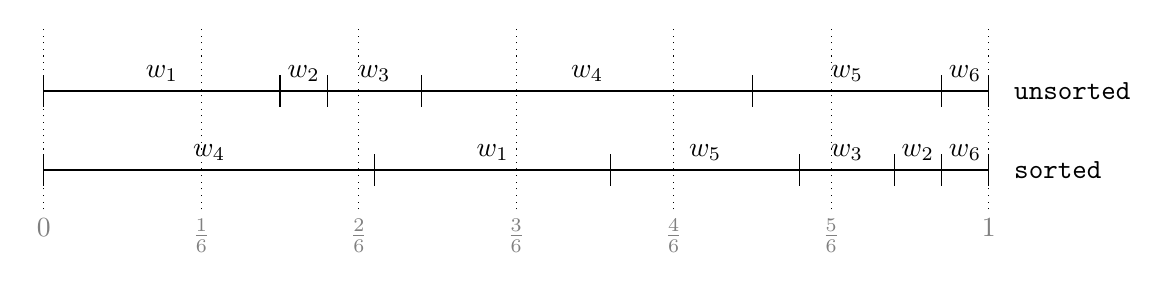
\begin{tikzpicture}
%% w = (0.25, 0.05, 0.10, 0.35, 0.20, 0.05)
%% vertical lines spaced 1/N apart
\draw[dotted] (0,-1.5) --(0,0.8);
\draw[dotted] (2,-1.5) --(2,0.8);
\draw[dotted] (4,-1.5) --(4,0.8);
\draw[dotted] (6,-1.5) --(6,0.8);
\draw[dotted] (8,-1.5) --(8,0.8);
\draw[dotted] (10,-1.5) --(10,0.8);
\draw[dotted] (12,-1.5) --(12,0.8);
%% labels for multiples of 1/N
\node[anchor=north, gray] at (0,-1.5) {$0$};
\node[anchor=north, gray] at (2,-1.5) {$\frac{1}{6}$};
\node[anchor=north, gray] at (4,-1.5) {$\frac{2}{6}$};
\node[anchor=north, gray] at (6,-1.5) {$\frac{3}{6}$};
\node[anchor=north, gray] at (8,-1.5) {$\frac{4}{6}$};
\node[anchor=north, gray] at (10,-1.5) {$\frac{5}{6}$};
\node[anchor=north, gray] at (12,-1.5) {$1$};
%% weight intervals, unsorted
\draw[thick] (0,0) -- (12,0);
\draw (0,-0.2) --(0,0.2);
\draw (3,-0.2) --(3,0.2);
\draw (3.6,-0.2) --(3.6,0.2);
\draw (4.8,-0.2) --(4.8,0.2);
\draw (9,-0.2) --(9,0.2);
\draw (11.4,-0.2) --(11.4,0.2);
\draw (12,-0.2) --(12,0.2);
%% weight labels, unsorted
\node[anchor=south] at (1.5,0) {$w_1$};
\node[anchor=south] at (3.3,0) {$w_2$};
\node[anchor=south] at (4.2,0) {$w_3$};
\node[anchor=south] at (6.9,0) {$w_4$};
\node[anchor=south] at (10.2,0) {$w_5$};
\node[anchor=south] at (11.7,0) {$w_6$};
%% weight intervals, sorted
\draw[thick] (0,-1) -- (12,-1);
\draw (0,-1.2) --(0,-0.8);
\draw (4.2,-1.2) --(4.2,-0.8);
\draw (7.2,-1.2) --(7.2,-0.8);
\draw (9.6,-1.2) --(9.6,-0.8);
\draw (10.8,-1.2) --(10.8,-0.8);
\draw (11.4,-1.2) --(11.4,-0.8);
\draw (12,-1.2) --(12,-0.8);
%% weight labels, sorted
\node[anchor=south] at (5.7,-1) {$w_1$};
\node[anchor=south] at (11.1,-1) {$w_2$};
\node[anchor=south] at (10.2,-1) {$w_3$};
\node[anchor=south] at (2.1,-1) {$w_4$};
\node[anchor=south] at (8.4,-1) {$w_5$};
\node[anchor=south] at (11.7,-1) {$w_6$};
%% labels sorted/unsorted
\node[anchor=west] at (12.2,0) {\texttt{unsorted}};
\node[anchor=west] at (12.2,-1) {\texttt{sorted}};
\end{tikzpicture}
\caption[Example where permuting weights can affect offspring counts]{An example in which permuting the weights can affect the conditional distribution of offspring counts under certain resampling schemes.
As in Figure~\ref{fig:inv_resampling}, $N=6$ and $w^{(1:6)} = (0.25,0.05,0.1,0.35,0.2,0.05)$.
The top row shows the weighted subintervals in the natural order, as in Figure~\ref{fig:inv_resampling}. 
The bottom row shows the partition corresponding to the same weights, but sorted in decreasing order. 
The dotted lines are spaced $1/N$ apart.
Under ``permutation-sensitive'' resampling schemes, the distribution of offspring counts differs depending on which partition is used.}
\label{fig:permutation_sensitivity}
\end{figure}

%\subsubsection{Sorting}
Related to this phenomenon, \textcite{gerber2017} prove some striking theoretical results concerning the effects of pre-sorting the particles. They show that sorting the particles in order of their states prior to resampling improves the rate of decay of resampling error from the usual $O(N^{-1})$ to $O(N^{-1-\frac{1}{d}})$, where $d$ is the dimension of the state space. 
In dimension $d=1$, this supports the numerical results of \textcite{kitagawa1996}, who observed empirically that sorting improved the convergence rate from $O(N^{-1})$ to $O(N^{-2})$ when working in one dimension.

In dimension $d\geq2$ things are more complicated because there is no full ordering of the state space. \textcite{gerber2017} get around this by mapping the state space onto $[0,1]^d$ and sorting by the Hilbert curve. 
The variance reduction from sorting the particles diminishes as the dimension increases, so in practice this has to be weighed up against the $O(N\log N)$ cost of sorting.

Another remarkable result of \textcite{gerber2017} is that, when the particles are sorted by their states, systematic resampling admits some theoretical support that was lacking in the unsorted case.
Recall that the possibly pathological behaviour of systematic resampling was related to ``bad'' orderings of the weight intervals; sorting the particles evidently prevents this.

The intuition behind these results is that sorting particles by their states ensures that the stratified and systematic resampling schemes select parents from a good range of locations in state space. The sorting step prevents the sampled parents being concentrated in one small part of the state space purely by a chance ordering of the weight intervals.
Another explanation \parencite{webber2019, li2020} is based on the observation that, under stratified or systematic resampling, the possible parents of a given offspring are always consecutive in the order in which the weights are input. Sorting these weights in order of the particle states ensures that these potential parents are ``close'' in state space, so that the state after resampling does not differ drastically depending on which parent is selected.

These results are only relevant to resampling schemes based on inversion sampling with fairly evenly-spaced points. Notably, multinomial resampling is not affected by sorting, since it is invariant under permutations of the weight vector.





\subsubsection{Computational complexity}
All of the resampling algorithms discussed in Section~\ref{sec:examples_resamplingschemes} can be implemented in $O(N)$ operations.
%\seb{Even \texttt{star} and \texttt{SSP} and \texttt{branching}? If it turns out to differ depending on resampling scheme then include it as a column in Table~\ref{tab:resampling_properties}. --- I think we can't say for \texttt{branching} becaue it dpeends on implementation, but \textcite[Corollary 18]{crisan1999} seems to imply $O(N^2)$...? SSP is definitely $O(N)$.}
Considering the complexity of each operation, \textcite{hol2006} suggest that systematic resampling is fastest because it only requires one pseudo-random number generation, and multinomial resampling is slower than stratified resampling because of the transformations required (although this may depend on which method is used to sample the Uniform order statistics). Residual resampling is hard to compare directly because a random fraction of the operations are deterministic, so the number of pseudo-random numbers required is a random number between $0$ and $N-1$, but the authors' simulation experiments place it between multinomial and stratified resampling.

However, the analysis of per-particle cost is sensitive to the particular implementation of each resampling scheme, the system implementation of pseudo-random number generation and arithmetic operations, and the hardware used, so it is not clear how robust such comparisons are.




\subsubsection{Negative association}
Following \textcite{gerber2017}, we use the definition of negative association from \textcite{joag1983}.
\begin{defn}
Let $(Z_1, \dots, Z_n)$ be a collection of random variables. 
$Z_{1:n}$ are said to be \emph{negatively associated} if, for every disjoint pair of subsets $I, J \subseteq \{1,\dots,n\}$, for all real-valued coordinatewise non-decreasing functions $\varphi, \psi$ for which the covariance is well defined,
\begin{equation*}
\Cov \left[ \varphi( Z_I) , \psi(Z_J) \right] \leq 0 .
\end{equation*}
\end{defn}
\textcite{gerber2017} show that negative association of offspring counts is a desirable property which may be used, along with some other machinery, to establish certain weak convergence results for the resampled measures.

Multinomial counts are negatively associated \parencite[Section 3.1]{joag1983}, which implies that residual-multinomial resampling also satisfies this property.
%\seb{Check that! Idea: deterministic parts have 0 correlation and the random parts are NA. Same goes for the other residual schemes mentioned below.}
\textcite{gerber2017} construct a counter-example to demonstrate that systematic resampling violates the negative association property.
For residual-systematic resampling, we can cook up a counterexample in the same spirit by taking $\varphi(x)=\psi(x)=\I{x=1}$, $I=\{1\}$, $J=\{3\}$ and considering a weight vector say $w^{(1:4)} = \frac{1}{8}(1,1,1,5)$ for $N=4$. Then the residual weights are $r^{(1:4)} = \frac{1}{4}(1,1,1,1)$ with $R=2$, so
\begin{align*}
\Cov \left[ \varphi( Z_I) , \psi(Z_J) \right]
&= \E[ \varphi( Z_I) \psi(Z_J) ] - \E[\varphi( Z_I) ] \E[\psi(Z_J) ] \\
&=\Prob[\nu^{(1)}=1, \nu^{(3)}=1] - \Prob[\nu^{(1)}=1] \Prob[\nu^{(3)}=1] \\
&= \frac{1}{2} - \frac{1}{2} \times \frac{1}{2} 
= \frac{1}{4}
>0 ,
\end{align*}
since the residual weight intervals corresponding to parents $1$ and $3$ both occupy the first half of a length-$(1/R)$ interval, hence $\{\nu^{(1)}=1\}$ and $\{\nu^{(3)}=1\}$ each have probability $1/2$ and $\nu^{(3)}=1$ if and only if $\nu^{(1)}=1$. 
So residual-systematic resampling also violates the negative association property.

\textcite{gerber2017} also mention some resampling schemes that do result in negatively associated counts: stratified resampling, and by implication residual-stratified resampling; star resampling (see the remark at the end of \textcite[Section 3.2]{gerber2017}), and by implication residual-star resampling.
The authors go on to introduce the SSP resampling scheme, which yields negatively associated offspring counts by construction.

These results are summarised in Table~\ref{tab:resampling_properties}.
The MVB algorithm does not enforce negative association, so this property depends on the particular implementation, and as such is left blank in Table~\ref{tab:resampling_properties}.







\subsubsection{Star discrepancy}
The \emph{star discrepancy} is a measure of the regularity of a given set of points $u_{1:N}$ in the unit hypercube. For our purposes it is sufficient to define the star discrepancy in one dimension, as in \textcite[Definition 1.2]{kuipers1974}:
\begin{equation}\label{eq:defn_stardiscrepancy}
D^\star (u_1, \dots, u_N)
:= \sup_{u \in [0,1]} | d(u) |
:= \sup_{u \in [0,1]} \left| u - \frac{1}{N} \sum_{i=1}^N \I{u_i \leq u} \right| .
\end{equation}
The quantity inside the supremum is the difference between the empirical CDF of the observed points $u_{1:N}$ and the CDF of the Uniform distribution on $[0,1]$.
Thus $D^\star$ measures, in a certain sense, how far the points are from being uniformly spaced.

\begin{figure}[ht]
\centering
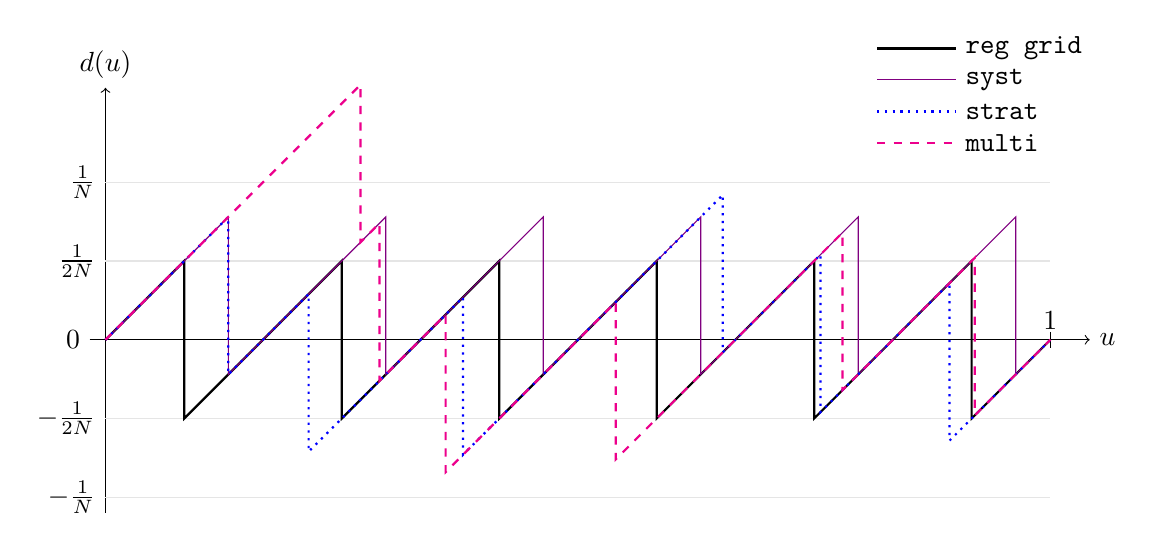
\begin{tikzpicture}
%% axes
\draw[->] (-0.2,0)--(12.5,0);
\draw[->] (0,-2.2)--(0,3.2);
\draw (12,0.1)--(12,-0.1);
\draw[gray!20] (0,1)--(12,1);
\draw[gray!20] (0,-1)--(12,-1);
\draw[gray!20] (0,2)--(12,2);
\draw[gray!20] (0,-2)--(12,-2);
%% axis labels
\node[anchor=west] at (12.5,0) {$u$};
\node[anchor=south] at (0,3.2) {$d(u)$};
\node[anchor=south] at (12,0) {$1$};
\node[anchor=east] at (-0.2,0) {$0$};
\node[anchor=east] at (0,1) {$\frac{1}{2N}$};
\node[anchor=east] at (0,-1) {$-\frac{1}{2N}$};
\node[anchor=east] at (0,2) {$\frac{1}{N}$};
\node[anchor=east] at (0,-2) {$-\frac{1}{N}$};
%% regular grid points
\draw[thick] (0,0)--(1,1)--(1,-1)--(3,1)--(3,-1)--(5,1)--(5,-1)--(7,1)--(7,-1)--(9,1)--(9,-1)--(11,1)--(11,-1)--(12,0);
%% systematic grid points, u as in Figure~\ref{fig:inv_resampling}
\draw[violet] (0,0)--(1.56,1.56)--(1.56,-0.44)--(3.56,1.56)--(3.56,-0.44)--(5.56,1.56)--(5.56,-0.44)--(7.56,1.56)--(7.56,-0.44)--(9.56,1.56)--(9.56,-0.44)--(11.56,1.56)--(11.56,-0.44)--(12,0);
%% stratified grid points, ditto
\draw[thick, blue, dotted] (0,0)--(1.56,1.56)--(1.56,-0.44)--(2.58,0.58)--(2.58,-1.42)--(4.54,0.54)--(4.54,-1.46)--(7.84,1.84)--(7.84, -0.16)--(9.08,1.08)--(9.08,-0.92)--(10.72,0.72)--(10.72,-1.28)--(12,0);
%% multinomial points, ditto
\draw[thick, magenta, dashed] (0,0)--(3.24,3.24)--(3.24,1.24)--(3.48,1.48)--(3.48,-0.52)--(4.32,0.32)--(4.32,-1.68)--(6.48,0.48)--(6.48,-1.52)--(9.36,1.36)--(9.36,-0.64)--(11.04,1.04)--(11.04,-0.96)--(12,0);
%% legend
\draw[thick, magenta, dashed] (9.8,2.5)--(10.8,2.5);
\node[anchor=west] at (10.8,2.5) {\texttt{multi}};
\draw[thick, blue, dotted] (9.8,2.9)--(10.8,2.9);
\node[anchor=west] at (10.8,2.9) {\texttt{strat}};
\draw[violet] (9.8,3.3)--(10.8,3.3);
\node[anchor=west] at (10.8,3.3) {\texttt{syst}};
\draw[thick] (9.8,3.7)--(10.8,3.7);
\node[anchor=west] at (10.8,3.7) {\texttt{reg grid}};
\end{tikzpicture}
\caption[Star discrepancy for multinomial, stratified and systematic resampling]{Plot of the function inside the absolute value in \eqref{eq:defn_stardiscrepancy}, for four different point sets. The points $u_{1:6}$ used are the same as in Figure~\ref{fig:inv_resampling}.\\
The solid black line corresponds to the regular grid, which achieves the minimal discrepancy $1/(2N)$, but cannot be used for resampling.
The star discrepancy of stratified and systematic points varies between $1/(2N)$ and $1/N$ depending on the realisation. In this example, the star discrepancy of the systematic points is $0.78/N$ and of the stratified points is $0.92/N$.
The star discrepancy of standard multinomial resampling (that is, i.i.d.\ Uniform points) can be arbitrarily close to $1$ for ``bad'' realisations; in this example it is $1.62/N$.}
\label{fig:star_discrepancy}
\end{figure}

Star discrepancy is used in quasi-Monte Carlo, where ``low-discrepancy'' points are used in place of Uniform random numbers to decrease the variance of Monte Carlo estimates.
We have noted already that resampling can itself be viewed as a Monte Carlo procedure.
From this point-of-view, stratified and systematic resampling are quasi-Monte Carlo implementations of multinomial resampling, since they provide ``more regular'' point sets to be used in inversion sampling.

In one dimension, the lowest-discrepancy point set is the regular grid $\frac{1}{2N}(1, 3, \dots, 2N-1)$, which has star discrepancy $\frac{1}{2N}$ \parencite[see for example][Corollary 1.2]{kuipers1974}.
However, resampling based on a deterministic point set cannot be unbiased since the resulting parental indices are conditionally deterministic given the weights.
Systematic resampling amounts to a randomisation of the regular grid, shifting each grid point by a random amount $u \sim \Unif[0,1/N]$, which corresponds to a randomised quasi-Monte Carlo procedure. This yields star discrepancy $D^\star = \max\{u, \frac{1}{N} -u\}$, which is between $1/(2N)$ and $1/N$ almost surely.
The point sets generated in stratified resampling also have star discrepancy between $1/(2N)$ and $1/N$, where the exact value depends on the realisation.
This certainly seems to improve on independent uniform points which can have star discrepancy arbitrarily close to $1$, the maximum possible value, albeit with diminishing probability as $N$ increases.
Figure~\ref{fig:star_discrepancy} illustrates how the star discrepancy is computed, and how it compares between these sampling methods.



\subsubsection{Matrix resampling}
Some resampling schemes render the parental indices $a_t^{(1:N)}$ conditionally independent over $i$ given the weights $w_t^{(1:N)}$, and such schemes admit a matrix representation conditional on the weights.
These resampling matrices are of particular interest in distributed SMC as they can be used to characterise the communication between particles required in the resampling step.
The matrices have been defined differently by different authors \parencite[cf.][]{webber2019, whiteley2016}, but the general idea is the same. Following most closely to the presentation of \textcite{li2020}, we use the following definition.

\begin{defn}
A \emph{resampling matrix} for weights $w_t^{(1:N)}$ is a $N\times N$ matrix with entries in $[0,1]$ such that:
\begin{enumerate}
\item each row sums to $1$, and
\item the $i^{th}$ column sums to $Nw_t^{(i)}$, for each $i \in \{1,\dots,N\}$.
\end{enumerate}
\end{defn}
The $ij^{th}$ element of the resampling matrix represents the conditional probability of offspring $i$ being resampled from parent $j$.
Some resampling schemes that are expressible as matrices are:
\begin{itemize}
\item no resampling, for which the resampling matrix is the identity matrix;
\item multinomial resampling, for which each row of the resampling matrix is the vector of weights;
\item stratified resampling;
\item residual-multinomial resampling;
\item residual-stratified resampling.
\end{itemize}
Illustrations of the structure of the resampling matrix resulting from each of these schemes can be found in \textcite[Figure 2]{li2020}, for example, although the residual resampling matrices may differ depending on the implementation.
All of the other resampling schemes we have encountered have some conditional dependence between the parental indices (as summarised in Table~\ref{tab:resampling_properties}) and thus are not representable by matrices.

Within the matrix resampling class, \textcite{li2020} show that, in one dimension, stratified resampling on the sorted particles is optimal in terms of the conditional variance \eqref{eq:resamplingMCvariance}, where sorting is based on the test function $\varphi$ applied to the states. They also prove that this scheme is optimal in other senses.
\textcite{webber2019} proves a generalisation to multiple dimensions: stratified resampling with the particles sorted by a certain functional of the states, based on $\varphi$, minimises the corresponding conditional variance.
The optimal functional by which to sort the particles cannot typically be computed, but the author suggests alternative sorting rules that also significantly improve performance, including the Hilbert curve sorting proposed by \textcite{gerber2017}.
%proves a similar result in multiple dimensions: stratified resampling on the particles sorted by a certain functional of the states is optimal in terms of conditional variance. As one might expect, the functional used for sorting is tailored to the test function $\phi$ over which the conditional variance is computed. 
\textcite{webber2019} also uses the matrix representations to construct alternative proofs of several of the results of Proposition~\ref{thm:resampling_var_compare}.

For our purposes, however, this class is too restrictive, as it excludes several resampling schemes that are prevalent in the literature and which perform comparably to, if not better than, conditionally independent resampling schemes.



%\subsubsection{Optimal resampling}
%\textcite{crisan1999} introduce another resampling scheme based on a branching process, which they show to be optimal in some sense. However, their algorithm is not widely used in practice because it is much more complicated to implement than alternatives like systematic resampling which perform just as well empirically, and share some of its optimality properties \parencite{bain2008}. 
%\seb{Possibly add an ``optimality'' column in Table~\ref{tab:resampling_properties} containing in what sense a scheme might be considered optimal.}



\begin{landscape}
\begin{table}[ht]
\centering
\begin{tabular}{ l | c c c c c c c c c }
\hline\hline
& \thead{support of $\nu_t^{(i)}$ given
            \\ $ \frac{K}{N} \leq w_t^{(i)} < \frac{K+1}{N}$} 
        & \thead{worst case\\ $|\nu_t^{(i)} - Nw_t^{(i)}|$}
        & \thead{degenerate if\\ $w_t^{(1:N)} =$\\ $\frac{1}{N}(1,\dots,1)$?} 
        & \thead{upper\\ bound on \\ $\V[\nu_t^{(i)}]$}
        & \thead{sensitive to\\ permutations\\ of weights?} 
        & \thead{PRNG\\ calls}
        & \thead{neg.\\ assoc.?}
        & \thead{cond.\\ indep.?} 
        & \thead{stochastic\\ rounding?}  \\
\hline
\texttt{multi} & $\{0,\dots,N\}$ & $N$ & $\times$ & $N/4$ 
        & $\times$ & $N$ & $\checkmark$ & $\checkmark$ & $\times$ \\
\texttt{star} & $\{0, N\}$ & $N$ & $\times$ & $N^2/4$ 
        & $\times$ & $1$ & $\checkmark$ & $\times$ & $\times$ \\
\texttt{strat} & $\{K-1, K, K+1, K+2\}$ & $2$ & $\checkmark$ & $2$ 
        & $\checkmark$ & $N$ & $\checkmark$ & $\checkmark$ & $\times$ \\
\texttt{syst} & $\{K, K+1\}$ & $1$ & $\checkmark$ & $1/4$ 
        & $\checkmark$ & $1$ & $\times$ & $\times$ & $\checkmark$ \\
\texttt{res-multi} & $\{K,\dots,N\}$ & $N-1$ & $\checkmark$  & $1$
        & $\times$ & $\leq N-1$ & $\checkmark$ & $\checkmark$ & $\times$ \\
\texttt{res-star} & $\{K, N\}$ & $N-1$ & $\checkmark$  & $N$
        & $\times$ & $1$ & $\checkmark$ & $\times$ & $\times$ \\
\texttt{res-strat} & $\{K, K+1, K+2\}$ & $2$ & $\checkmark$  & $1/2$
        & $\checkmark$ & $\leq N-1$ & $\checkmark$ & $\checkmark$ & $\times$ \\
\texttt{res-syst} & $\{K, K+1\}$ & $1$ & $\checkmark$ & $1/4$ 
        & $\checkmark$ & $1$ & $\times$ & $\times$ & $\checkmark$ \\
\texttt{ssp} & $\{K, K+1\}$ & $1$ & $\checkmark$ & $1/4$
        & $\times$ & $\leq N$ & $\checkmark$ & $\times$ & $\checkmark$ \\
%\texttt{mvb} & $\{K, K+1\}$ & $1$ & $1/4$ & $\checkmark$ & $\checkmark$ 
%        & & & \\
\hline\hline
\end{tabular}
\caption[Properties of resampling schemes]{Summary of some of the properties of resampling schemes explored in Section~\ref{sec:resampling_properties}. 
Columns appear in order of their explanations in the text.
The abbreviated names for the resampling schemes are explained in Table~\ref{tab:resampling_abbrevs}.}
%Some properties are not specified for \texttt{mvb} because they depend on the particular implementation.
\label{tab:resampling_properties}
\end{table} 
\end{landscape}
 
 
 

\subsection{Stochastic rounding}
\label{sec:SRs}
Some of the resampling schemes we have met can be classified as \emph{stochastic roundings}. This will be useful later on, as we will see (Section~\ref{sec:convergenceSRs}) that all members of this class admit some common convergence results.
The stochastic roundings class is a subclass of MVB resampling (Section~\ref{sec:examples_resamplingschemes}) additionally constrained to satisfy condition \ref{item:resampling_property1} of Definition~\ref{defn:resampling}.

\begin{defn}\label{defn:stochround}
 Let $X=(X_1,\dots,X_N)$ be a $\mathbb{R}_+^N$-valued random variable. Then $Y=(Y_1,\dots,Y_N) \in \mathbb{N}^N$ is a \emph{stochastic rounding} of $X$ if each element $Y_i$ takes values
\begin{equation*}
Y_i \mid X_i =
\begin{cases}
 \lfloor X_i \rfloor & \text{with probability } 1- X_i+ \lfloor X_i \rfloor \\
  \lfloor X_i \rfloor +1 & \text{with probability } X_i- \lfloor X_i \rfloor .
\end{cases}
\end{equation*}
\end{defn}

By construction, $\E(Y_i) = X_i$ for each $i$. Taking $X$ to be $N$ times the vector of particle weights, we can therefore use stochastic rounding to construct a valid resampling scheme, under the further constraint that $Y_1 + \dots + Y_N = N$.
Several ways to enforce this constraint on the joint distribution have been proposed, including systematic resampling, residual resampling with systematic residuals, and SSP resampling.

Explicitly, the offspring counts are marginally distributed according to 
\begin{equation*}
\nu_t^{(i)} \mid w_t^{(i)}
\eqdist \flnw + \Bern( Nw_t^{(i)} - \flnw ) .
\end{equation*}

Some of the properties discussed earlier are common to every stochastic rounding scheme. 
Since all such schemes give offspring counts with the same marginal distributions, properties such as the marginal offspring variance are common to all stochastic roundings. Indeed it is easy to see that the marginal variance of the offspring counts, $\V[ \nu_t^{(i)} \mid w_t^{(i)} ]$ is as small as possible under the constraint of unbiasedness, and as such this is sometimes referred to as minimal-variance resampling.
By definition, the support of an offspring count $\nu_t^{(i)}$ given that the associated weight lies in the interval $K/N \leq w_t^{(i)} < (K+1)/N$ is $\{ K, K+1\}$. 
All stochastic roundings are also degenerate when the weights are all equal, i.e.\ $w_t^{(1:N)} = (1,\dots, 1)/N$ implies $\nu_t^{(1:N)}=(1,\dots,1)$ almost surely.





\section{Conditional SMC}
\label{sec:condSMC}
%\seb{Be consistent with upper/lower case letters: $X,x$ etc.}\\
\textcite{andrieu2010} propose a number of ``particle MCMC'' algorithms, which combine SMC with MCMC in order to improve performance in certain situations.
One of their algorithms, the \emph{particle Gibbs} sampler \parencite[Section 2.4.3]{andrieu2010}, is of particular interest in the current work. For one thing, genealogies are particularly critical to its performance, and for another, the particle update uses a variant SMC algorithm which alters the distribution of genealogies.

In this section, we first introduce the particle Gibbs algorithm and the conditional SMC update, then discuss how ancestral degeneracy impacts the performance of particle Gibbs and how ancestor sampling mitigates this.




\subsection{Particle Gibbs}
\label{sec:particleGibbs}
To motivate the particle Gibbs algorithm, we introduce a parametrised state space model and explain how combining SMC updates with MCMC sampling allows us to tackle the related inferences effectively.
The particle Gibbs algorithm can be applied much more broadly, but this application is particularly intuitive and exhibits all the features of interest to our genealogical study.

Consider a parametrised state space model of the form
\begin{align*}
\theta &\sim p(\cdot) & \\
X_0 &\sim \mu^\theta(\cdot) & \\
X_{t+1} \mid X_{t} &\sim K_{t+1}^\theta(\cdot \mid X_{t}) &\text{for } t=0,\dots, T-1 \\
Y_t \mid X_t &\sim g_t^\theta(\cdot \mid X_t) &\text{for } t=0,\dots, T
\end{align*}
exactly like \eqref{eq:SSM_spec} except that the specification is now parametrised by $\theta$ (which may be multi-dimensional), and we place a prior distribution on $\theta$. 
As usual, $p$, $\mu^\theta$, $(K_t^\theta)$ and $(g_t^\theta)$ are part of the model and are assumed to be known but not necessarily tractable.

Suppose that, given some data $y_{0:T}$, we wish to generate Monte Carlo samples from the joint posterior distribution of $X_{0:T}$ and $\theta$. (Even if we are only interested in inferring $\theta$, for instance, it is often more practical to target the joint posterior and then marginalise.)
Notice that we are now working with a finite time horizon $T\in\mathbb{N}$. The inference of interest here is not inherently sequential; we are building an MCMC algorithm to sample from a single target distribution which happens to include some sequentially correlated components.


The conditional dependence structure of the model invites the use of a Gibbs sampler, sampling alternately from the conditional distributions $p(\theta \mid x_{0:T}, y_{0:T})$ and $p(x_{0:T} \mid \theta, y_{0:T})$.
The $\theta$ update,
\begin{equation*}
p(d\theta \mid x_{0:T}, y_{0:T}) \propto p(d\theta) p(x_{0:T}, y_{0:T} \mid \theta) ,
\end{equation*}
is often quite straightforward, if not analytically then by employing a Metropolis-Hastings step based on the current sampled values of $\theta$ and $x_{0:T}$. 
The $X$ update, meanwhile, is high-dimensional with strong sequential correlations: exactly the situation in which one might use SMC. 
For the $X$ update, we need a sample from
\begin{equation}\label{eq:PG_Xposterior}
p(dx_{0:T} \mid \theta, y_{0:T}) 
\propto \mu^\theta(dx_0) g_0^\theta(y_0\mid x_0) \prod_{s=1}^T K_s^\theta(dx_s \mid x_{s-1}) g_s^\theta(y_s \mid x_s) ,
\end{equation}
which can be approximately obtained by running an SMC smoother then sampling one trajectory from its output in proportion to the associated weight.

However, the Markov chain associated to the procedure just described does not admit $p(x_{0:T},\theta \mid y_{0:T})$ as an invariant distribution. It \emph{approximately} targets this distribution, with some bias.
A Gibbs sampler targeting $p(x_{0:T},\theta \mid y_{0:T})$ exactly can be constructed by replacing the SMC step with a \emph{conditional SMC} step, which takes into account the value of $x_{0:T}$ sampled at the previous iteration, as well as the observations and the current value of $\theta$.

A conditional SMC algorithm for this scenario is presented in Algorithm~\ref{alg:condSMC}.
In contrast to Algorithm~\ref{alg:SMC}, the input now includes $x_{0:T}^\star$ and $a_{0:T}^\star$, which encode the states and parental indices, respectively, of the \emph{immortal trajectory} (so called because it ``survives'' the SMC run with probability one). Within a particle Gibbs algorithm, the immortal trajectory is set to the trajectory sampled at the previous iteration.
The resampling step now assigns the immortal offspring to the immortal parent deterministically, and the state of the immortal particle is also updated deterministically rather than via the Markov kernel.
As in standard SMC, there is a choice of \textsc{resample} procedures, but some care is needed to ensure the correct treatment of the immortal particle \parencite[for details see e.g.][]{lee2019}.
In the case of multinomial resampling, exchangeability of the offspring means that conditioning on $a_{t-1}^\star$ has no effect on the resampling of the non-immortal particles.

\begin{algorithm}[ht]
\vspace*{10pt}
\DontPrintSemicolon
\KwIn{$T, N, \mu^\theta, (K_t^\theta), (g_t^\theta), y_{0:T}, x_{0:T}^\star, a_{0:T}^\star$}
Set $X_0^{(a_0^\star)} \gets x_0^\star$\;
\lFor{$i \in \{1,\dots,N\} \setminus a_0^\star$}{
	Sample $X_0^{(i)} \sim \mu(\cdot)$
}
\lFor{$i \in \{1,\dots, N\}$}{
		$w_{0}^{(i)} \gets \left\{ {\sum_{j=1}^N g_0^\theta(y_0 \mid X_0^{(j)})}\right \}^{-1}{g_0^\theta(y_0 \mid X_0^{(i)})} $
}                
\For{$t \in \{1,\dots, T\}$}{
	Set $a_{t-1}^{(a_{t}^\star)} \gets a_{t-1}^\star$, 	$X_{t}^{(a_{t}^\star)} \gets x_{t}^\star$\;
        Sample $a_{t-1}^{(1:N)}\setminus a_{t-1}^\star \sim \textsc{resample}(\{1,\dots,N\}, w_{t-1}^{(1:N)} \mid a_{t-1}^\star)$\;
	\lFor{$i \in \{1,\dots,N\} \setminus a_t^\star$}{
		Sample $X_{t}^{(i)} \sim K_{t}^\theta( \cdot \mid X_{t-1}^{(a_{t-1}^{(i)})} )$
	}
    	\lFor{$i \in \{1,\dots, N\}$}{	
		$w_{t}^{(i)} \gets \Big\{ {\sum_{j=1}^N g_{t}^\theta(y_{t} \mid X_{t}^{(j)}) }\Big\}^{-1} g_{t}^\theta(y_{t} \mid X_{t}^{(i)}) $
	}          
}
\vspace*{10pt}
\caption[Conditional sequential Monte Carlo]{Conditional sequential Monte Carlo for a parametrised state space model. The immortal particle at each generation has its new state and parental index set deterministically according to the values of $x_{0:T}^\star$ and $a_{0:T}^\star$ given as input.}
\label{alg:condSMC}
\end{algorithm}
The complete particle Gibbs algorithm for this example then consists of alternately sampling from the full conditional distribution of $\theta$ (e.g.\ using a Metropolis-Hastings update) and sampling a trajectory $(x_{0:T}, a_{0:T})$ using conditional SMC. See \textcite[Section 2.4.3]{andrieu2010} for more details.




\subsection{Ancestral degeneracy in particle Gibbs}
We have seen in Section~\ref{sec:SMC_genealogies} that the phenomenon of ancestral degeneracy can severely affect the performance of SMC algorithms, particularly in smoothing applications.
The SMC update of particle Gibbs is a smoothing problem, however it requires only one sampled trajectory from the smoothing distribution, so one might imagine that we are safe from the curse of ancestral degeneracy.
In fact, the loss of ancestors causes a different problem for particle Gibbs: it prevents some components of the Markov chain being refreshed, so that the chain mixes slowly.

To see this, consider the illustration in Figure~\ref{fig:PG_ancdegen}, which shows the smoothing trajectories generated by a conditional SMC update at some iteration $r$. The thick black line is the immortal trajectory given as input, that is, the trajectory sampled by the conditional SMC update at iteration $r-1$. Backwards in time, the sampled trajectories quickly coalesce until at time $20$ all of the trajectories have coalesced. The common trajectory from time $0$ to $20$ must necessarily be part of the immortal trajectory.
A new trajectory (highlighted in purple) is then sampled among the $N$ generated trajectories. Whichever trajectory we sample, it will certainly overlap with the previously sampled trajectory at least from time $0$ to $20$.

\begin{figure}[ht]
\centering
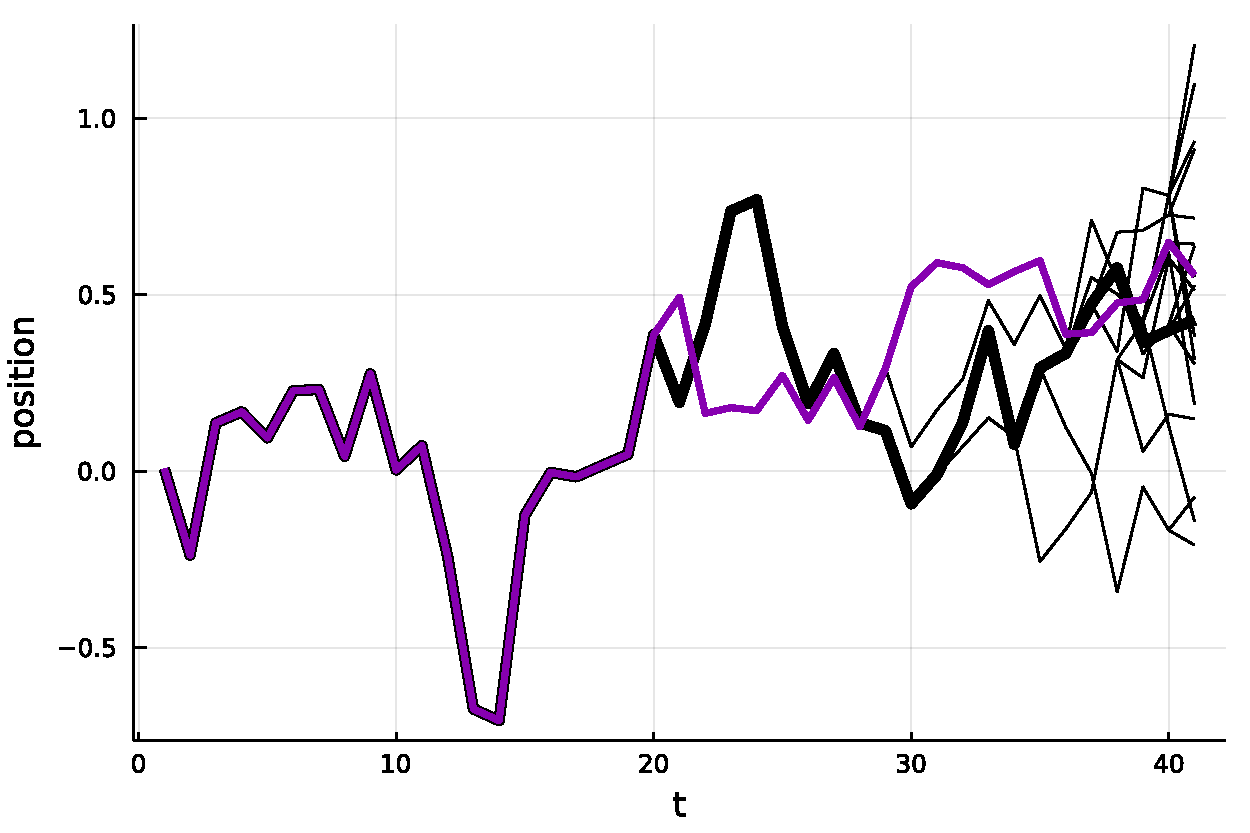
\includegraphics[width=0.8\textwidth]{plots/PG_degen.pdf}
\caption[Ancestral degeneracy in particle Gibbs]{Illustration of how ancestral degeneracy causes particle Gibbs to mix slowly on some components. The thick black line is the immortal trajectory, i.e.\ the sampled trajectory from the previous iteration. Other lines are all of the trajectories generated by conditional SMC. One of these (highlighted in purple) is the sampled trajectory at the current iteration. Due to ancestral degeneracy, the current sample (purple) coincides with the previous sample (thick black) up to time 20, so the components $x_{0:20}$ are not updated in this iteration.}
\label{fig:PG_ancdegen}
\end{figure}

At the next iteration the newly sampled trajectories will again coalesce onto the immortal trajectory, and this behaviour is repeated. 
If $T$ is too large with respect to $N$, the early part of the trajectory will very rarely be updated, so the corresponding states will mix very slowly.
For further intuition on this phenomenon the reader is directed to \textcite[Section 5.4]{lindsten2013}.
%\seb{Also include a plot showing sticky realisations from a sequence of consecutive draws?}
%\seb{If the immortal trajectory is not ``typical'' of the target smoothing distribution, then the new lineages tend not to degenerate very quickly onto the immortal lineage, which would solve this problem. However, since the immortal trajectory is supposed to be (approaching) a sample from the target, this is not much comfort. Perhaps if perturbing $\theta$ profoundly changes the model? But I don't think that kind of instability is desirable either.}

The meaning of $T$ ``too large'' here depends on the model and the type of SMC update used, but typically $T$ is determined by the application and $N$ is limited by computational resources, so we may not be able to control their relative size. The other brute-force approach would be to increase the number of iterations of the MCMC algorithm, but this too is infeasible on a limited computational budget.
It is therefore worth investing some effort to find an alternative solution to the problem of ancestral degeneracy within particle Gibbs.





\subsection{Ancestor sampling}\label{sec:ancsamp}
An effective solution (where it is possible to implement it) was proposed by \textcite{whiteley2010} and is known as \emph{ancestor sampling}.
It consists of a simple modification to the resampling step within the conditional SMC algorithm. 
In the basic algorithm with multinomial resampling, at each time step the non-immortal particles are resampled by multinomial resampling according to their weights, while the immortal offspring is deterministically assigned to the immortal parent. That is, at time $t$, for each $i \in \{1,\dots, N\}$,
\begin{equation*}
\Prob[a_t^{(j)} = i \mid X_{0:t}^{(1:N)}, x_{0:T}^\star, a_{0:T}^\star ] 
\propto \begin{cases}
w_t^{(i)} & j \text{ non-immortal} \\
\I{i = a_t^\star} & j \text{ immortal} .
\end{cases}
\end{equation*}

Ancestor sampling combines the resampling step with a backward simulation step for the immortal particle. Instead of deterministically inheriting the ``correct'' parent, the immortal particle samples its parent among all $N$ possible parents.
This is justified in the same way as backwards simulation in general (Section~\ref{sec:anc_degen}), provided the ancestor sampling probabilities are chosen correctly, although we now apply the backwards sampling step to the immortal trajectory only.
Ancestor sampling can also be implemented for other choices of \textsc{resample}, using the same backward simulation probabilities (but of course the resampling probabilities for non-immortal particles will be different, and there may be some additional dependence between parental indices). For simplicity we here restrict ourselves to multinomial resampling.

\begin{algorithm}[ht]
\vspace*{10pt}
\DontPrintSemicolon
\KwIn{$T, N, \mu^\theta, (K_t^\theta), (q_t^\theta), (g_t^\theta), y_{0:T}, x_{0:T}^\star, a_{0:T}^\star$}
Set $X_0^{(a_0^\star)} \gets x_0^\star$\;
\lFor{$i \in \{1,\dots,N\} \setminus a_0^\star$}{
	Sample $X_0^{(i)} \sim \mu^\theta(\cdot)$
}
\lFor{$i \in \{1,\dots, N\}$}{
		$w_{0}^{(i)} \gets  \left\{ {\sum_{j=1}^N g_0^\theta(y_0 \mid X_0^{(j)})}\right \}^{-1}{g_0^\theta(y_0 \mid X_0^{(i)})} $
}                
\For{$t \in \{1,\dots, T\}$}{
	Set $X_{t}^{(a_{t}^\star)} \gets x_{t}^\star$\;
	Sample $a_{t-1}^{(a_{t}^\star)} \sim \Cat\left( \{1,\dots,N\}, w_{t-1}^{(1:N)} q_{t}^\theta(x_{t}^\star \mid X_{t-1}^{(1:N)}) \right)$\;
        Sample $a_{t-1}^{(1:N)}\setminus a_{t-1}^\star \sim \textsc{resample}(\{1,\dots,N\}, w_{t-1}^{(1:N)} \mid a_{t-1}^\star)$\;
	\lFor{$i \in \{1,\dots,N\} \setminus a_t^\star$}{
		Sample $X_{t}^{(i)} \sim K_{t}^\theta( \cdot \mid X_{t-1}^{(a_{t-1}^{(i)})} )$
	}
    	\lFor{$i \in \{1,\dots, N\}$}{	
		$w_{t}^{(i)} \gets \Big\{ {\sum_{j=1}^N g_{t}^\theta( y_{t} \mid X_{t}^{(j)}) }\Big\}^{-1} g_{t}^\theta( y_{t} \mid X_{t}^{(i)}) $
	}          
}
\vspace*{10pt}
\caption[Conditional sequential Monte Carlo with ancestor sampling]{Conditional sequential Monte Carlo with ancestor sampling for a parametrised state space model. The parent of the immortal particle is updated at each iteration via an on-line backward simulation step. The transition kernels $K_t^\theta$ are assumed to admit densities $q_t^\theta$. The second parameter of the Categorical variable should be interpreted element-wise, and is given up to a normalisation constant.}
\label{alg:condSMC_ancsamp}
\end{algorithm}
Assume that the smoothing distributions admit densities, that is $\mu^\theta(\cdot)$ and $K_t^\theta(\cdot\mid x)$ admit densities for all $x,t$. Denote the density of $K_t^\theta$ by $q_t^\theta$. Define the trajectories $X_{t, 0:t}^{(i)}$ (for any $t,i$) as in Section~\ref{sec:SMC_FK}, starting from $X_{t,t}^{(i)} := X_t^{(i)}$ and tracing back the states of the parents via $X_{t,s}{(i)} = X_{t,s+1}^{( a_t^{(i)} )}$.
Then the correct resampling probabilities are, for each $i$,
\begin{equation}\label{eq:ancsamp_probs}
\Prob[a_t^{(j)} = i \mid X_{0:t}^{(1:N)}, x_{0:T}^\star, a_{0:T}^\star ] 
\propto \begin{cases}
w_t^{(i)} & j \text{ non-immortal}\\
w_t^{(i)} \frac{
        p( (X_{t,0:t}^{(i)}, x_{t+1:T}^\star) \mid \theta, y_{0:T} )}
        {p( X_{t,0:t}^{(i)} \mid \theta, y_{0:t} ) } 
        & j \text{ immortal} .
\end{cases}
\end{equation}
The ratio of densities can be interpreted as the conditional probability that the whole trajectory is the concatenation of $X_{t,0:t}^{(i)}$ with $x_{t+1:T}^\star$, given that its first $t+1$ states are $X_{t,0:t}^{(i)}$.
To simplify the ratio, use \eqref{eq:PG_Xposterior} to write
\begin{equation*}
p( X_{t,0:t}^{(i)} \mid \theta, y_{0:t} )
\propto \mu^\theta( X_{t,0}^{(i)} ) g_0^\theta( y_0 \mid X_{t,0}^{(i)} ) 
        \prod_{s=1}^{t} q_s^\theta( X_{t,s}^{(i)} \mid X_{t,s-1}^{(i)} ) 
        g_s^\theta( y_s \mid X_{t,s}^{(i)} )
\end{equation*}
and %\seb{actually, this explicit trajectory notation is going to make all this much heavier... but perhaps it's worth it for the clarity?}
\begin{align*}
&p( (X_{t,0:t}^{(i)}, x_{t+1:T}^\star) \mid \theta, y_{0:T} ) \\
&\qquad \propto \mu^\theta( X_{t,0}^{(i)} ) g_0^\theta( y_0 \mid X_{t,0}^{(i)} ) 
        \left\{ \prod_{s=1}^{t} q_s^\theta( X_{t,s}^{(i)} \mid X_{t,s-1}^{(i)} )
        g_s^\theta( y_s \mid X_{t,s}^{(i)} ) \right\} \\
    &\hspace{2cm}\times q_{t+1}^\theta( x_{t+1}^\star \mid X_{t,t}^{(i)} ) 
        g_{t+1}^\theta( y_{t+1} \mid x_{t+1}^\star )
        \left\{ \prod_{s=t+2}^T q_s^\theta(x_s^\star \mid x_{s-1}^\star)
        g_s^\theta(y_s \mid x_s^\star) \right\} .
\end{align*}
The ratio then becomes
%\seb{I think the first proportionality hides the likelihood ratio $p(y_{0:T}|\theta)/p(y_{0:t-1}|\theta)$ --- see \eqref{eq:PG_Xposterior} --- it might make things clearer if I keep such constants explicit for longer?}
\begin{align*}
&\frac{p( ( X_{t,0:t}^{(i)}, x_{t+1:T}^\star ) \mid \theta, y_{0:T} )}
        {p( X_{t,0:t}^{(i)} \mid \theta, y_{0:t} ) } \\
&\qquad\qquad\propto q_{t+1}^\theta( x_{t+1}^\star \mid X_{t,t}^{(i)} ) 
        g_{t+1}^\theta( y_{t+1} \mid x_{t+1}^\star )
        \prod_{s=t+2}^T q_s^\theta( x_s^\star \mid x_{s-1}^\star ) 
        g_s^\theta( y_s \mid x_s^\star ) \\
&\qquad\qquad\propto q_{t+1}^\theta( x_{t+1}^\star \mid X_{t,t}^{(i)} )
        = q_{t+1}^\theta( x_{t+1}^\star \mid X_{t}^{(i)} )  .
\end{align*}
The probabilities in \eqref{eq:ancsamp_probs} become
\begin{equation}\label{eq:ancsamp_probs_simplified}
\Prob[a_t^{(j)} = i \mid X_{0:t}^{(1:N)}, x_{0:T}^\star, a_{0:T}^\star ] 
\propto \begin{cases}
w_t^{(i)} & j \text{ non-immortal}\\
w_t^{(i)} q_{t+1}^\theta( x_{t+1}^\star \mid X_{t}^{(i)} ) & j \text{ immortal} .
\end{cases}
\end{equation}
The conditional SMC algorithm with this adaptation is presented in Algorithm~\ref{alg:condSMC_ancsamp}.

We see that, in order to do ancestor sampling, we need a stronger assumption on the Markov kernels than was required to simply run the conditional SMC algorithm: we now require that, for each $t$, $K_t^\theta$ admits a density $q_t^\theta$ and that $q_t^\theta(\cdot \mid x)$ can be evaluated pointwise for any $x$, whereas previously we only needed to draw samples from $K_t^\theta(\cdot\mid x)$ for any $x$.
This additional requirement rules out ancestor sampling in some applications, for instance when the transitions are discretisations of some stochastic differential equation.

Recall that the usual backward simulation procedure requires a full forward pass to calculate the future states before the backward simulation probabilities can be computed. Ancestor sampling, on the other hand, does not require a forward pass because it only computes backward simulation probabilities for the immortal trajectory, for which all the future states are known in advance. This means that the additional computational cost of implementing ancestor sampling is negligible.




\subsubsection{Why ancestor sampling works}
We know that complete backward simulation eradicates ancestral degeneracy by sampling each lineage independently (Section~\ref{sec:anc_degen}).
But here we are only backward-simulating one of the $N$ particles, leaving the other $N-1$ lineages to coalesce as usual. So how does this help?

Recall that in particle Gibbs ancestral degeneracy is not itself a problem, because we only require a single sample from the smoothing distribution. 
The problem is that the consecutive samples are highly correlated, because of  the repeated coalescence onto the immortal lineage.
The contribution of ancestor sampling is to break up the immortal trajectory so that it no longer appears among the lineages; see Figure~\ref{fig:whyASworks}. While the non-immortal trajectories may still coalesce, they no longer preferentially coalesce onto the immortal trajectory. 
In turn, the sampled trajectory that is output does not overlap unduly with the immortal trajectory that was the previous output, and this completely solves the problem of the slow-mixing particle Gibbs chain.

\begin{figure}[ht]
\centering
\subfloat[without ancestor sampling]{
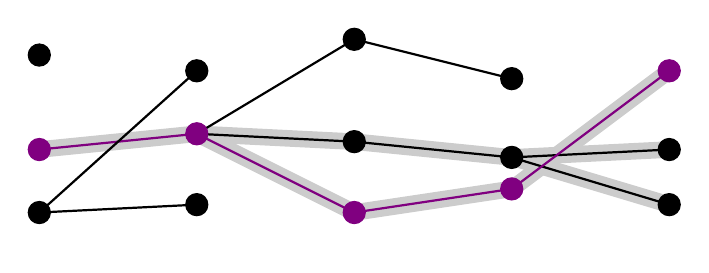
\begin{tikzpicture}
% highlight lineage 1 (immortal lineage)
\draw[line width=6pt, gray!40] (0,0.8)--(2,1);
\draw[line width=6pt, gray!40] (2,1)--(4,0);
\draw[line width=6pt, gray!40] (4,0)--(6,0.3);
\draw[line width=6pt, gray!40] (6,0.3)--(8,1.8);
% highlight lineage 2
\draw[line width=6pt, gray!40] (2,1)--(4,0.9);
\draw[line width=6pt, gray!40] (4,0.9)--(6,0.7);
\draw[line width=6pt, gray!40] (6,0.7)--(8,0.8);
% highlight lineage 3
\draw[line width=6pt, gray!40] (6,0.7)--(8,0.1);
%
% lines column 1-2
\draw[thick] (0,0)--(2,0.1);
\draw[thick, violet] (0,0.8)--(2,1);
\draw[thick] (0,0)--(2,1.8);
% lines column 2-3
\draw[thick, violet] (2,1)--(4,0);
\draw[thick] (2,1)--(4,0.9);
\draw[thick] (2,1)--(4,2.2);
% lines column 3-4
\draw[thick, violet] (4,0)--(6,0.3);
\draw[thick] (4,0.9)--(6,0.7);
\draw[thick] (4,2.2)--(6,1.7);
% lines column 4-5
\draw[thick] (6,0.7)--(8,0.1);
\draw[thick] (6,0.7)--(8,0.8);
\draw[thick, violet] (6,0.3)--(8,1.8);
%
% nodes column 1
\filldraw (0,0) circle (4pt);
\filldraw[violet] (0,0.8) circle (4pt);
\filldraw (0,2) circle (4pt);
% nodes column 2
\filldraw (2,0.1) circle (4pt);
\filldraw[violet] (2,1) circle (4pt);
\filldraw (2,1.8) circle (4pt);
% nodes column 3
\filldraw[violet] (4,0) circle (4pt);
\filldraw (4,0.9) circle (4pt);
\filldraw (4,2.2) circle (4pt);
% nodes column 4
\filldraw[violet] (6,0.3) circle (4pt);
\filldraw (6,0.7) circle (4pt);
\filldraw (6,1.7) circle (4pt);
% nodes column 5
\filldraw (8,0.1) circle (4pt);
\filldraw (8,0.8) circle (4pt);
\filldraw[violet] (8,1.8) circle (4pt);
% fake line to add space
\draw[white] (0,-0.4)--(1,-0.4);
\end{tikzpicture}
\label{fig:whyASworks_a}
}\\
\subfloat[with ancestor sampling]{
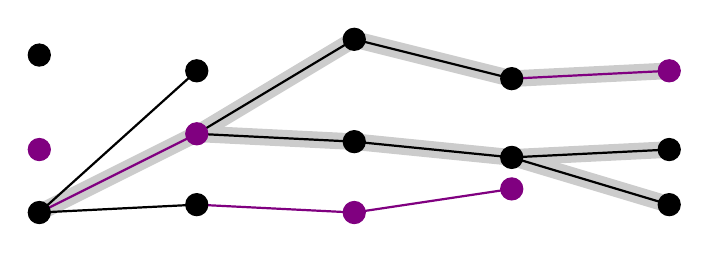
\begin{tikzpicture}
% highlight lineage 1
\draw[line width=6pt, gray!40] (0,0)--(2,1);
\draw[line width=6pt, gray!40] (2,1)--(4,2.2);
\draw[line width=6pt, gray!40] (4,2.2)--(6,1.7);
\draw[line width=6pt, gray!40] (6,1.7)--(8,1.8);
% highlight lineage 2
\draw[line width=6pt, gray!40] (2,1)--(4,0.9);
\draw[line width=6pt, gray!40] (4,0.9)--(6,0.7);
\draw[line width=6pt, gray!40] (6,0.7)--(8,0.8);
% highlight lineage 3
\draw[line width=6pt, gray!40] (6,0.7)--(8,0.1);
%
% lines column 1-2
\draw[thick] (0,0)--(2,0.1);
\draw[thick, violet] (0,0)--(2,1);
\draw[thick] (0,0)--(2,1.8);
% lines column 2-3
\draw[thick, violet] (2,0.1)--(4,0);
\draw[thick] (2,1)--(4,0.9);
\draw[thick] (2,1)--(4,2.2);
% lines column 3-4
\draw[thick, violet] (4,0)--(6,0.3);
\draw[thick] (4,0.9)--(6,0.7);
\draw[thick] (4,2.2)--(6,1.7);
% lines column 4-5
\draw[thick] (6,0.7)--(8,0.1);
\draw[thick] (6,0.7)--(8,0.8);
\draw[thick, violet] (6,1.7)--(8,1.8);
%
% nodes column 1
\filldraw (0,0) circle (4pt);
\filldraw[violet] (0,0.8) circle (4pt);
\filldraw (0,2) circle (4pt);
% nodes column 2
\filldraw (2,0.1) circle (4pt);
\filldraw[violet] (2,1) circle (4pt);
\filldraw (2,1.8) circle (4pt);
% nodes column 3
\filldraw[violet] (4,0) circle (4pt);
\filldraw (4,0.9) circle (4pt);
\filldraw (4,2.2) circle (4pt);
% nodes column 4
\filldraw[violet] (6,0.3) circle (4pt);
\filldraw (6,0.7) circle (4pt);
\filldraw (6,1.7) circle (4pt);
% nodes column 5
\filldraw (8,0.1) circle (4pt);
\filldraw (8,0.8) circle (4pt);
\filldraw[violet] (8,1.8) circle (4pt);
% fake line to add space
\draw[white] (0,-0.4)--(1,-0.4);
\end{tikzpicture}
\label{fig:whyASworks_b}
}
\caption[Why ancestor sampling works]{Illustration of how ancestor sampling prevents coalescence onto the immortal trajectory. Immortal particles are highlighted in purple, along with their parent-offspring edges (the given ones in \subref{fig:whyASworks_a} and the ancestor-sampled ones in \subref{fig:whyASworks_b}). The resulting lineages of the terminal particles are highlighted in grey. 
In \subref{fig:whyASworks_a}, the lineages of the terminal particles coalesce onto the immortal trajectory. Imagine time stretching further back: the lineages would continue to coincide with the immortal trajectory forever. 
In \subref{fig:whyASworks_b}, the lineages still coalesce, but not onto the immortal trajectory. The immortal trajectory no longer exists as a lineage.}
\label{fig:whyASworks}
\end{figure}


